%--------------------------------------------------------------------%
%
% Berkas utama templat LaTeX.
%
% author Petra Barus, Peb Ruswono Aryan, Faris Rizki Ekananda
%
%--------------------------------------------------------------------%
%
% Berkas ini berisi struktur utama dokumen LaTeX yang akan dibuat.
%
%--------------------------------------------------------------------%

\documentclass[bahasa, 12pt, a4paper, onecolumn, oneside, final]{report}

%-------------------------------------------------------------------%
%
% Konfigurasi dokumen LaTeX untuk laporan tesis IF ITB
%
% @author Petra Novandi
%
%-------------------------------------------------------------------%
%
% Berkas asli berasal dari Steven Lolong
%
%-------------------------------------------------------------------%

% Ukuran kertas
\special{papersize=210mm,297mm}

% Setting margin
\usepackage[top=2cm,bottom=2cm,left=4cm,right=3cm]{geometry}

% Math package
\usepackage{mathptmx}

% 4th Sectioning
\usepackage{titlesec}
\newcommand{\subsubsubsection}[1]{\paragraph{#1}\mbox{}\\}

\titleformat{\subsubsubsection}
{\normalfont\normalsize\bfseries}{\theparagraph}{1em}{}
\titlespacing*{\subsubsubsection}
{0pt}{3.25ex plus 1ex minus .2ex}{1.5ex plus .2ex}

% Judul bahasa Indonesia
\usepackage[bahasa]{babel}

% Format citation
\usepackage[utf8]{inputenc}
\usepackage[style=apa,backend=biber]{biblatex}
\usepackage{longtable}
\usepackage{graphicx}
\usepackage{subfig}
\usepackage{titling}
\usepackage{booktabs}
\usepackage{tabularx}
\usepackage{blindtext}
\usepackage{sectsty}
\usepackage{chngcntr}
\usepackage{etoolbox}
\usepackage{array}
\usepackage[hidelinks]{hyperref}       % Package untuk link di daftar isi. Ubah jadi \usepackage[hidelinks]{hyperref} apabila ingin menghilangkan kotak merah disekitar link
\usepackage{titlesec}       % Package Format judul
\usepackage{titletoc}       % Package Format judul di toc
\usepackage{tocbibind}      % Package untuk masukkan toc, lot, lof ke Daftar Isi
\usepackage{scrwfile}       % Package untuk membuat Daftar Lampiran dari toc
\usepackage{parskip}
\usepackage{afterpage}
\usepackage{relsize}
\usepackage{xcolor, colortbl}
\usepackage{setspace}
\usepackage{listings}

\graphicspath{{resources/}}   % letak direktori penyimpanan gambar

% Setting daftar lampiran
\newcommand*{\lopname}{DAFTAR LAMPIRAN}
\TOCclone[\lopname]{toc}{atoc}
\addtocontents{atoc}{\protect\value{tocdepth}=-1}
\newcommand\listofappendices{
	\cleardoublepage
	\phantomsection
	\listofatoc
	\addcontentsline{toc}{chapter}{\lopname}
}

\newcommand*\savedtocdepth{}
\AtBeginDocument{%
	\edef\savedtocdepth{\the\value{tocdepth}}%
}

\let\originalappendix\appendix
\renewcommand\appendix{%
	\originalappendix
	\cleardoublepage
	\addtocontents{toc}{\protect\value{tocdepth}=-1}%
	\addtocontents{atoc}{\protect\value{tocdepth}=\savedtocdepth}%

	\titlecontents{chapter}
	[0pt]
	{\bfseries}
	{Lampiran \thecontentslabel.\quad}
	{}
	{\hfill\contentspage}

	\titleformat{\chapter}[block]
	{\bfseries}
	{\chaptertitlename\ \thechapter.\quad}{0pt}
	{\bfseries}
}

% Hilangkan titik pada toc
\makeatletter
\renewcommand{\@dotsep}{1}
\makeatother

% Setel title pada chapter-chapter di toc, lof, lot
\titlecontents{chapter}
[0pt]
{\bfseries}
{\MakeUppercase{Bab} \thecontentslabel\quad\uppercase}
{}
{\mdseries\titlerule*[0.35em]{.}\bfseries\contentspage}
\titlecontents{figure}
[0pt]
{}
{Gambar \thecontentslabel.\quad}
{}
{\mdseries\titlerule*[0.35em]{.}\bfseries\contentspage}
\titlecontents{table}
[0pt]
{}
{Tabel \thecontentslabel.\quad}
{}
{\mdseries\titlerule*[0.35em]{.}\bfseries\contentspage}

% Masukin Daftar Pustaka ke toc
\let\originalprintbibliography\printbibliography
\renewcommand\printbibliography{%
	\phantomsection
	\cleardoublepage
	\originalprintbibliography
	\addcontentsline{toc}{chapter}{\bibname}
}

% Line satu setengah spasi
\renewcommand{\baselinestretch}{1.5}

% Setting judul
\chapterfont{\centering \large}
\titleformat{\chapter}[display]
{\Large\centering\bfseries}
{\chaptertitlename\ \thechapter}{0pt}
{\Large\bfseries\uppercase}

% Setting nomor pada subbsubsubbab
\setcounter{secnumdepth}{4}

\makeatletter

\makeatother

% Counter untuk figure dan table.
\counterwithin{figure}{chapter}
\counterwithin{table}{chapter}

% Define blank page
\newcommand*{\blankpage}{\afterpage{\null\newpage}}

% Translate autoref into Indonesian
\renewcommand*{\equationautorefname}{Persamaan}%
\renewcommand*{\footnoteautorefname}{catatan kaki}%
\renewcommand*{\itemautorefname}{item}%
\renewcommand*{\figureautorefname}{Gambar}%
\renewcommand*{\tableautorefname}{Tabel}%
\renewcommand*{\partautorefname}{Bagian}%
\renewcommand*{\appendixautorefname}{Lampiran}%
\renewcommand*{\chapterautorefname}{Bab}%
\renewcommand*{\sectionautorefname}{Subbab}%
\renewcommand*{\subsectionautorefname}{Subsubbab}%
\renewcommand*{\subsubsectionautorefname}{Subsubsubbab}%
\renewcommand*{\paragraphautorefname}{paragraf}%
\renewcommand*{\subparagraphautorefname}{subparagraf}%
\renewcommand*{\FancyVerbLineautorefname}{garis}%
\renewcommand*{\theoremautorefname}{Teorema}%
\renewcommand*{\pageautorefname}{halaman}%

% Format to ignore underflow hbadness
\hbadness=99999
%--------------------------------------------------------------------%
%
% Hypenation untuk Bahasa Indonesia
%
% @author Petra Barus
%
%--------------------------------------------------------------------%
%
% Secara otomatis LaTeX dapat langsung memenggal kata dalam dokumen,
% tapi sering kali terdapat kesalahan dalam pemenggalan kata. Untuk
% memperbaiki kesalahan pemenggalan kata tertentu, cara pemenggalan
% kata tersebut dapat ditambahkan pada dokumen ini. Pemenggalan
% dilakukan dengan menambahkan karakter '-' pada suku kata yang
% perlu dipisahkan.
%
% Contoh pemenggalan kata 'analisa' dilakukan dengan 'a-na-li-sa'
%
%--------------------------------------------------------------------%

\hyphenation {
	% A
	%
	a-na-li-sa
	a-pli-ka-si
	a-lo-ka-si
	an-ta-ra
	ada-nya
	akan
	% B
	%
	be-be-ra-pa
	ber-ge-rak
	be-ri-kut
	ber-ko-mu-ni-ka-si
	buah
	Bouvet
	ber-fo-kus
	ber-fung-si
	ber-ja-lan
	% C
	%
	ca-ri
	Carzaniga
	cloud
	CloudFormation
	con-tai-ner
	ClusterIP
	% D
	%
	da-e-rah
	di-nya-ta-kan
	de-fi-ni-si
	di-bu-tuh-kan
	di-gu-na-kan
	di-tam-bah-kan-nya
	di-tem-pat-kan
	di-la-ku-kan
	di-kem-bang-kan
	di-im-ple-men-ta-si-kan
	da-pat
	di-ka-te-go-ri-kan
	de-ngan
	di-kem-bang-kan
	da-ta
	% E
	%
	e-ner-gi
	eks-klu-sif
	eks-ter-nal
	% F
	%
	fa-si-li-tas
	% G
	%
	ga-bung-an
	% H
	%
	ha-lang-an
	ha-sil
	hell
	% I
	% 
	i-nduk
	in-for-ma-si
	im-ple-men-tasi
	% J
	%
	% K
	%
	kom-po-si-si
	ka-re-na
	ke-sa-ba-ran-nya
	ka-me-ra
	kua-li-tas
	ke-na-ngan
	kom-plek-si-tas
	ke-ti-ka
	ke-le-bi-han-nya
	ke-gi-a-tan
	ko-mu-ni-ka-si
	ke-cil
	% L
	%
	la-ya-nan
	% M
	%
	me-ngu-ra-ngi
	meng-eva-lu-a-si
	me-nge-lo-la
	men-da-lam
	men-ja-lan-kan
	mak-si-mal
	me-nye-le-sai-kan
	me-ngunjungi
	men-du-kung
	me-nu-rut
	me-la-ku-kan
	mem-buat
	men-daftar-kan
	me-ngu-sul-kan
	me-mi-li-ki
	meng-gu-na-kan
	men-ja-di
	me-ru-pa-kan
	men-ja-ga
	me-mu-dah-kan
	me-ne-rus-
	mem-pro-ses
	% N
	%
	Na-mun
	% O
	%
	ob-so-lete
	or-kes-tra-si
	oto-ma-ti-sa-si
	% P
	%
	pro-vi-der
	pe-ru-sa-ha-an
	pe-rang-kat
	pro-ses
	plat-form
	pro-duk-si
	pe-ne-li-tian
	pe-ru-ba-han
	pa-ra-dig-ma
	pe-man-tau-an
	pe-ngum-pu-lan
	pa-ckage
	% Q
	%
	quality
	% R
	%
	% S
	se-la-in
	stan-dar-di-sasi
	se-cu-ri-ty
	so-lu-si
	se-lu-ruh
	Soft-ware
	soft-ware
	se-buah
	se-ca-ra
	%
	% T
	% 
	ter-li-bat
	ter-pi-sah-kan
	ter-mi-nal
	ter-ba-tas
	% U
	%
	un-tuk
	% V
	%
	% W
	%
	% X
	%
	% Y
	% 
	% Z
	%
}

%--------------------------------------------------------------------%
%
% Hypenation untuk Bahasa Inggris
%
% @author Muhammad Garebaldhie ER Rahman
%
%--------------------------------------------------------------------%
%
% LaTeX can automatically hyphenate words within a document,
% but often there are errors in the hyphenation. To
% correct specific hyphenation errors, the desired hyphenation
% can be added to this document. Hyphenation is done by
% adding the character '-' between the syllables to be separated.
%
% For example, the word 'constrained' can be hyphenated as 'con-strained'.
%
%--------------------------------------------------------------------%

\hyphenation {
	% A
	%
	% B
	%
	% C
	%
	con-strained
	% D
	%
	de-ploy-ment
	de-activation
	% E
	%
	% F
	%
	% G
	%
	% H
	%
	% I
	% 
	% J
	%
	% K
	%
	% L
	%
	% M
	%
	% N
	%
	% O
	%
	% P
	%
	% Q
	%
	% R
	%
	re-source
	re-mote
	% S
	%
	% T
	% 
	% U
	%
	% V
	%
	% W
	%
	% X
	%
	% Y
	% 
	% Z
	%
	zoo-keeper
}


\makeatletter

\makeatother

\addbibresource{references.thesis.bib}
\hyphenpenalty=5000
\tolerance=1000

\begin{document}

\title{Pengembangan \textit{Smart Contract Discovery System} Berbasis Semantik dengan Menggunakan \textit{Large Language Model} dan \textit{Retrieval-Augmented Generation}}
\date{}
\author{
	Kenneth Ezekiel Suprantoni \\
	NIM: 13521089
}
\newcommand\tanggalpengesahan{XXX XXX 2025}

\pagenumbering{roman}
\setcounter{page}{1}

\clearpage
\pagestyle{empty}

\begin{center}
	\smallskip

	\Large \bfseries \MakeUppercase{\thetitle}
	\vfill

	\Large Laporan Tugas Akhir
	\vfill

	\large Disusun sebagai syarat kelulusan tingkat sarjana
	\vfill

	\large Oleh

	\Large \theauthor

	\vfill
	\begin{figure}[ht]
		\centering
		
\includegraphics[width=0.15\textwidth]{cover-ganesha.jpg}
	\end{figure}
	\vfill

	\large
	\uppercase{
		Program Studi Teknik Informatika \\
		Sekolah Teknik Elektro \& Informatika \\
		Institut Teknologi Bandung
	}

	Juli 2025

\end{center}

\clearpage

\clearpage
\pagestyle{empty}

\begin{center}
	\smallskip

	\Large \bfseries \MakeUppercase{\thetitle}
	\vfill

	\Large Laporan Tugas Akhir
	\vfill

	\large Oleh

	\Large \theauthor

	\large Program Studi Teknik Informatika \\

	\normalsize \normalfont
	Sekolah Teknik Elektro dan Informatika \\
	Institut Teknologi Bandung \\

	\vfill
	\normalsize \normalfont

	% Telah disetujui dan disahkan sebagai Laporan Tugas Akhir \\
	Telah disetujui dan disahkan sebagai Laporan Tugas Akhir \\
	di Bandung, pada tanggal \tanggalpengesahan

	\vspace{0.5cm}
	Pembimbing,

	\vfill
	\underline{Dr. techn. Muhammad Zuhri Catur Candra, S.T, M.T.
	} \\
	NIP. 19770921 201012 1 002

\end{center}
\clearpage

\chapter*{Lembar Pernyataan}

Dengan ini saya menyatakan bahwa:

\begin{enumerate}

	\item Pengerjaan dan penulisan Laporan Tugas Akhir ini dilakukan tanpa menggunakan bantuan yang tidak dibenarkan.
	\item Segala bentuk kutipan dan acuan terhadap tulisan orang lain yang digunakan di dalam penyusunan Laporan Tugas Akhir ini telah dituliskan dengan baik dan benar.
	\item Laporan Tugas Akhir ini belum pernah diajukan pada program pendidikan di perguruan tinggi mana pun.

\end{enumerate}

Jika terbukti melanggar hal-hal di atas, saya bersedia dikenakan sanksi sesuai dengan Peraturan Akademik dan Kemahasiswaan Institut Teknologi Bandung bagian Penegakan Norma Akademik dan Kemahasiswaan khususnya Pasal 2.1 dan Pasal 2.2.
\vspace{15mm}

Bandung, \tanggalpengesahan

\vspace{1.5cm}
Kenneth Ezekiel Suprantoni \\
NIM 13521089


\pagestyle{plain}

% \clearpage
\chapter*{ABSTRAK}
\addcontentsline{toc}{chapter}{ABSTRAK}
\begin{center}
	\center
	\begin{singlespace}
		\large\bfseries\MakeUppercase{\thetitle}

		\normalfont\normalsize
		Oleh:

		\bfseries \theauthor
	\end{singlespace}
\end{center}

\begin{singlespace}
	\small

    % Di tengah pertumbuhan data Smart Contracts dalam blockchain, kebutuhan untuk sebuah sistem pencarian yang mengakomodasi penggunaan ulang semakin meningkat.
	% Pertumbuhan adopsi blockchain dan peningkatan jumlah Smart Contracts di dalam ekosistem blockchain menciptakan tantangan-tantangan baru. Salah satu tantangan utamanya adalah untuk menggunakan kembali Smart Contracts yang telah ada yang sesuai dengan kebutuhan. Sistem pencarian Smart Contracts saat ini masih mengandalkan pencarian berbasis kata kunci atau teks yang kurang mempertimbangkan konteks semantik dari kontrak tersebut. Sehingga, pengguna masih sulit untuk menemukan Smart Contracts yang sesuai dengan kebutuhan mereka. Pada tugas akhir ini dikembangkan sebuah Smart Contract Discovery System berbasis konteks semantik yang memanfaatkan kemampuan LLM untuk mendeskripsikan \textit{source code} dari sebuah kontrak secara semantik dan melakukan pengambilan data menggunakan kemiripan semantik. Sistem ini memanfaatkan Distributed Graph Database (Dgraph) untuk menyimpan data kontrak dan embeddings yang merepresentasikan kontrak tersebut. Sistem ini mengintegrasikan modul ekstraksi data, \textit{enrichment} data, pemodelan data, dan \textit{retrieval} data untuk meningkatkan relevansi hasil pencarian. Hasil evaluasi menunjukkan bahwa sistem ini mampu meningkatkan presisi dalam menemukan kontrak yang relevan dibandingkan dengan pendekatan tradisional. Dengan demikian, rancangan ini membuktikan efektivitas penggunaan konteks semantik dalam penemuan Smart Contracts pada ekosistem blockchain.

	Smart Contracts sudah diadopsi secara luas dan terdapat kebutuhan untuk berinteraksi atau menggunaka ulang kontrak yang sudah ada. Sistem saat ini menggunakan mekanisme pencarian yang bersifat leksikal, yang bertumpu pada ketersesuaian sintaks, yang tidak selalu merepresentasikan fungsi dan maksud dari kontrak. Terdapat beberapa sistem yang sudah mengeksplorasi pendekatan untuk mendeskripsikan fungsi dan maksud dari sebuah kontrak, tetapi sistem-sistem tersebut tidak terintegrasi secara \textit{end-to-end} dari ekstraksi sampai pencarian dan belum memanfaatkan LLM modern dengan kapabilitasnya untuk menganalisis dan mengerti fungsi dari sebuah kode. 
	
	Pada tugas akhir ini dikembangkan sebuah Smart Contract Discovery System berbasis konteks semantik, yang merupakan sebuah \textit{pipeline} dari ekstraksi data Smart Contracts pada Blockchain Ethereum, ekstraksi deskripsi semantik dari Smart Contracts tersebut menggunakan LLM modern dengan struktur yang modular sehingga dapat mengganti model dengan mudah, lalu memasukkan data ke sebuah repositori yang dapat dilakukan pencarian secara semantik menggunakan \textit{cosine similarity} dari \textit{embeddings} antar kueri dan data. Hasil evaluasi menunjukkan bahwa sistem ini mampu menemukan Smart Contracts dengan kategori yang dimaksud dari kueri pengguna dari hasil ekstraksi Smart Contracts yang terdapat di blockchain dan terdapat peningkatan presisi saat dibandingkan dengan sistem pencarian berbasis teks. Dengan demikian, rancangan ini membuktikan efektivitas sistem pencarian berbasis semantik dalam penemuan Smart Contracts pada ekosistem blockchain.

	\textbf{\textit{Kata kunci: Smart Contracts, Sistem Pencarian, Semantik, LLM, Enrichment, Embeddings, Retrieval}}

\end{singlespace}
\clearpage
% \clearpage
\chapter*{ABSTRACT}
\addcontentsline{toc}{chapter}{ABSTRACT}

\begin{center}
	\center
	\begin{singlespace}
		\large\bfseries\MakeUppercase{Judul TA Disini}

		\normalfont\normalsize
		By:

		\bfseries \theauthor
	\end{singlespace}
\end{center}

\begin{singlespace}
	\small
	Lorem Ipsum is simply dummy text of the printing and typesetting industry. Lorem Ipsum has been the industry's standard dummy text ever since the 1500s, when an unknown printer took a galley of type and scrambled it to make a type specimen book. It has survived not only five centuries, but also the leap into electronic typesetting, remaining essentially unchanged. It was popularised in the 1960s with the release of Letraset sheets containing Lorem Ipsum passages, and more recently with desktop publishing software like Aldus PageMaker including versions of Lorem Ipsum.

	It is a long established fact that a reader will be distracted by the readable content of a page when looking at its layout. The point of using Lorem Ipsum is that it has a more-or-less normal distribution of letters, as opposed to using 'Content here, content here', making it look like readable English. Many desktop publishing packages and web page editors now use Lorem Ipsum as their default model text, and a search for 'lorem ipsum' will uncover many web sites still in their infancy. Various versions have evolved over the years, sometimes by accident, sometimes on purpose (injected humour and the like).

	Contrary to popular belief, Lorem Ipsum is not simply random text. It has roots in a piece of classical Latin literature from 45 BC, making it over 2000 years old. Richard McClintock, a Latin professor at Hampden-Sydney College in Virginia, looked up one of the more obscure Latin words, consectetur, from a Lorem Ipsum passage, and going through the cites of the word in classical literature, discovered the undoubtable source. Lorem Ipsum comes from sections 1.10.32 and 1.10.33 of "de Finibus Bonorum et Malorum" (The Extremes of Good and Evil) by Cicero, written in 45 BC. This book is a treatise on the theory of ethics, very popular during the Renaissance. The first line of Lorem Ipsum, "Lorem ipsum dolor sit amet..", comes from a line in section 1.10.32.

	\textbf{\textit{Keywords: Lorem, Ipsum, Lorem Ipsum }}
\end{singlespace}
\clearpage

\clearpage

\chapter*{Kata Pengantar}
\addcontentsline{toc}{chapter}{KATA PENGANTAR}

Puji dan syukur penulis panjatkan kepada Tuhan Yang Maha Esa 

% \begin{enumerate}
% 	\item 
% \end{enumerate}


\begin{flushright}
	\vspace{0.5cm}
	Bandung, \tanggalpengesahan

	\vspace{1.5cm}

	Kenneth Ezekiel Suprantoni
\end{flushright}


% Puji dan syukur penulis panjatkan kepada Tuhan Yang Maha Esa atas berkat dan rahmatnya, laporan tugas akhir yang berjudul "\thetitle" dapat diselesaikan dalam rangka memenuhi syarat kelulusan tingkat sarjana. Perlu diakui pengerjaan tugas akhir ini didukung oleh banyak pihak. Khususnya, penulis ingin mengucapkan terima kasih kepada:

% \begin{enumerate}
% 	\item Bapak Dr.techn. Muhammad Zuhri Catur Candra, S.T., M.T., selaku dosen pembimbing atas segala bentuk dukungan yang telah diberikan dan kesabarannya dalam membimbing penulis serta memberikan saran dalam pengerjaan tugas akhir.
% 	\item Bapak Yudistira Dwi Wardhana Asnar, S.T, Ph.D dan Dr. Agung Dewandaru, S.T., M.Sc., selaku dosen penguji atas segala masukan dan kritik yang telah diberikan terhadap tugas akhir penulis.
% 	\item Dicky Prima Satya, S.T, M.T., Bapak Adi Mulyanto, S.T, M.T., Robithoh Annur, S.T., M.Eng., Ph.D., dan Tricya Esterina Widagdo, ST., M.Sc. selaku dosen koordinator tim tugas akhir atas usahanya mengingatkan mahasiswa program studi Teknik Informatika untuk mengerjakan tugas akhirnya.
% 	\item Seluruh dosen program studi Teknik Informatika ITB yang telah memberikan ilmu pengetahuan yang sangat berharga bagi penulis.
% 	\item Ibu Rini Liani dan Bapak Edhie Hikmat selaku kedua orangtua penulis atas dukungan yang diberikan
% 	\item Rumah Amal Salman ITB serta tim Beasiswa Perintis yang telah membantu penulis sehingga penulis dapat menempuh pendidikan di Institut Teknologi Bandung dengan mudah.
% 	\item Teman-teman INIT 2020 yang telah menemani, memberikan inspirasi, serta dukungan moral kepada penulis dalam menempuh kuliah pada program studi Teknik Informatika.
% 	\item Teman-teman penulis khususnya anggota dari grup "temenin ngerjain TA", "Koordinasi penonton sempro", "Para Ajudan Pecinta Sedekah", "Kos Aufa Enjoyer", "kaliMANTAN", serta "karimun" yang telah memberikan kenangan berharga, motivasi, hiburan, serta bantuan untuk segala situasi.
% 	\item Sahabat Penulis khususnya Erik dan Rachel yang telah pantang menyerah berjuang bersama dalam berkompetisi CTF.
% 	\item Sahabat terdekat penulis khususnya Marcho, Aira, Gagas, Rio, Dhika, Kinan, Anca, Dipa, Ubai, Azka, Sarah, Dea, Fay, Epi, Aufa, Syahrul, Rifqi dan Malik yang telah menemani perjuangan dari TPB hingga saat ini, menjadi \textit{emotional support} di segala situasi, membantu penulis dalam proses pengejaan tugas akhir, serta membuat hari - hari menjadi lebih berwarna.
% 	\item Seluruh pihak lain yang tidak bisa disebutkan disini yang telah membantu dalam proses pengerjaan tugas akhir.
% \end{enumerate}

% Akhir kata, penulis mengucapkan terima kasih kepada semua pihak yang telah terlibat dalam pengerjaan tugas akhir ini. Penulis juga ingin menyampaikan mohon maaf apabila terdapat kesalahan maupun kekurangan dalam laporan tugas akhir ini. Penulis berharap semoga tugas akhir ini dapat bermanfaat bagi pembaca dan riset-riset kedepannya.

\titleformat*{\section}{\centering\bfseries\Large\MakeUpperCase}
\titlespacing*{\chapter}{0pt}{0pt}{4pt}

% Setting judul toc, lot, lof, bib
\renewcommand{\contentsname}{DAFTAR ISI}
\renewcommand{\listfigurename}{DAFTAR GAMBAR}
\renewcommand{\listtablename}{DAFTAR TABEL}
\renewcommand{\bibname}{DAFTAR PUSTAKA}

% daftar isi, lampiran, gambar, table
\tableofcontents
\listofappendices
\listoffigures
\listoftables

\newpage

\titleformat*{\section}{\bfseries\large}
\pagenumbering{arabic}

%----------------------------------------------------------------%
% Konfigurasi Bab
%----------------------------------------------------------------%
\setcounter{page}{1}
\renewcommand{\chaptername}{BAB}
\renewcommand{\thechapter}{\Roman{chapter}}
%----------------------------------------------------------------%

%----------------------------------------------------------------%
% Dafter Bab
% Untuk menambahkan daftar bab, buat berkas bab misalnya `chapter-6` di direktori `chapters`, dan masukkan ke sini.
%----------------------------------------------------------------%
\chapter{Pendahuluan}

% Bab Pendahuluan secara umum yang dijadikan landasan kerja dan arah kerja penulis tugas akhir, berfungsi mengantar pembaca untuk membaca laporan tugas akhir secara keseluruhan.

% \section{Latar Belakang}
% \label{sec:latarbelakang}

% Latar Belakang berisi dasar pemikiran, kebutuhan atau alasan yang menjadi ide dari topik tugas akhir. Tujuan utamanya adalah untuk memberikan informasi secukupnya kepada pembaca agar memahami topik yang akan dibahas.  Saat menuliskan bagian ini, posisikan anda sebagai pembaca – apakah anda tertarik untuk terus membaca?

% \section{Rumusan Masalah}

% Rumusan Masalah berisi masalah utama yang dibahas dalam tugas akhir. Rumusan masalah yang baik memiliki struktur sebagai berikut:

% \begin{enumerate}
% 	\item Penjelasan ringkas tentang kondisi/situasi yang ada sekarang terkait dengan topik utama yang dibahas Tugas Akhir.
% 	\item Pokok persoalan dari kondisi/situasi yang ada, dapat dilihat dari kelemahan atau kekurangannya. \textbf{Bagian ini merupakan inti dari rumusan masalah}.
% 	\item Elaborasi lebih lanjut yang menekankan pentingnya untuk menyelesaikan pokok persoalan tersebut.
% 	\item Usulan singkat terkait dengan solusi yang ditawarkan untuk menyelesaikan persoalan.
% \end{enumerate}

% Penting untuk diperhatikan bahwa persoalan yang dideskripsikan pada subbab ini akan dipertanggungjawabkan di bab Evaluasi apakah terselesaikan atau tidak.

% \section{Tujuan}

% Tuliskan tujuan utama dan/atau tujuan detil yang akan dicapai dalam pelaksanaan tugas akhir. Fokuskan pada hasil akhir yang ingin diperoleh setelah tugas akhir diselesaikan, terkait dengan penyelesaian persoalan pada rumusan masalah. Penting untuk diperhatikan bahwa tujuan yang dideskripsikan pada subbab ini akan dipertanggungjawabkan di akhir pelaksanaan tugas akhir apakah tercapai atau tidak.

% \section{Batasan Masalah}

% Tuliskan batasan-batasan yang diambil dalam pelaksanaan tugas akhir. Batasan ini dapat dihindari (tidak perlu ada) jika topik/judul tugas akhir dibuat cukup spesifik.

% \section{Metodologi}

% Tuliskan semua tahapan yang akan dilalui selama pelaksanaan tugas akhir. Tahapan ini spesifik untuk menyelesaikan persoalan tugas akhir. Tahapan studi literatur tidak perlu dituliskan karena ini adalah pekerjaan yang harus Anda lakukan selama proses pelaksanaan tugas akhir.

% \section{Jadwal Pelaksanaan Tugas Akhir}

% Tuliskan rencana kegiatan dan jadwal (dirinci sampai per minggu) mulai dari awal pelaksanaan Tugas Akhir I s.d. sidang tugas akhir berikut milestones dan deliverables yang harus diberikan. Jadwal ini dapat dibantu dengan membuat sebuah tabel timeline.
\section{Related Work}\label{sec:related}

\subsection{Smart Contract Indexing and Analysis}
Several research efforts have focused on extracting and indexing blockchain data to improve accessibility. Third and Domingue~\cite{b4} proposed using Linked Data principles to create a semantic index for Ethereum, mapping blockchain entities to an ontology. The Graph Protocol~\cite{b5} offers a decentralized indexing solution where ``subgraphs'' can be defined to query specific on-chain data via a GraphQL API. While powerful for querying transactional data, these systems do not focus on the semantic content of the contract code itself.

For code analysis, tools have emerged to make sense of compiled bytecode. The STAN system~\cite{b6} aimed to describe the functionality of closed-source contracts by analyzing their bytecode. Similarly, the eth2dgraph tool~\cite{b7}, which we utilize in our work, can decompile bytecode to extract a contract's Application Binary Interface (ABI) using heimdall-rs. However, these approaches are limited by the information loss that occurs during compilation and do not capture the high-level design intent available in source code. Furthermore, there is no present research that has explored utilizing LLM's capability to analyze source code into analyzing smart contracts' source code.

\subsection{Semantic Code Search}
The application of Natural Language Processing (NLP) to code search has gained traction. Zhang~\cite{b8} developed a ``Solidity Summarizer'' using transformer models to generate natural language comments for Solidity code, aiming to improve readability. Shi et al.~\cite{b9} proposed MM-SCS, a multi-modal search model that combines textual features with structural information from a ``Contract Elements Dependency Graph'' to improve search accuracy. These methods show the promise of semantic understanding but often require complex model training and do not integrate into a complete, end-to-end discovery system.

\subsection{Gap Analysis}
Our work builds upon these foundations but addresses a critical gap. While previous systems focused on either indexing transactions or analyzing code structure, our approach leverages the advanced reasoning capabilities of modern LLMs to create a rich, structured semantic layer directly from source code. Furthermore, our work focuses on a real data pipeline, utilizing eth2dgraph capability to extract the full blockchain data into the database. By integrating this pipeline, complete with deep semantic enrichment into a scalable architecture featuring a graph database and vector search, we provide a full-fledged discovery system that allows developers to find contracts based on what they do, not just what words they contain.
\chapter{Analisis Masalah dan Rancangan Solusi}

Bab ini akan berisikan deskripsi detail terkait persoalan, rencana penyelesaian persoalan, dan solusi yang akan dibangun dalam tugas akhir. Bab ini diharapkan dapat memberikan gambaran jelas pada persoalan yang dibahas dan solusi yang akan dibangun.

% Tujuan utama penulisan bab ini adalah untuk menguraikan rencana penyelesaian masalah tugas akhir I.. Bab ini mencakup antara lain: 
% 1.	Deskripsi dan analisis persoalan yang terkait dengan Rumusan Masalah, misalnya menjelaskan secara detail latar belakang dan masalah yang menjadi dasar munculnya topik, menunjukkan gap/celah antara kondisi saat ini dengan kondisi yang diharapkan, dan kaitan antara sistem/aplikasi yang dikembangkan dengan sistem/aplikasi lain yang terkait.
% 2.	Analisis solusi yang terdiri dari pilihan alternatif solusi yang dapat digunakan untuk setiap permasalahan berdasarkan hasil studi literatur atau survei, pemilihan solusi beserta justifikasinya.
% 3.	Deskripsi umum solusi yang dipilih, mencakup:
% a.	Modul/subsistem/komponen yang akan dikembangkan untuk menyelesaikan masalah, berikut penjelasannya.
% b.	Alur umum algoritma atau langkah-langkah pengembangan sistem dan penjelasannya.
% c.	Penggunaan kakas yang diperlukan
% Dianjurkan untuk menggunakan diagram sebagai pendukung penjelasan bagian ini.

\section{Analisis}

\subsection{Analisis Masalah}
\label{subsec:analisis-masalah}

% Dalam pengembangan dApps, Smart Contracts berperan sebagai \textit{building blocks} yang saling terhubung dan berinteraksi sesuai dengan fungsionalitasnya. Namun, dengan jumlah Smart Contracts yang terus bertambah di blockchain dan ketiadaan mekanisme klasifikasi yang jelas, pemilihan Smart Contracts yang tepat menjadi tantangan yang kompleks. Kesulitan ini terutama muncul dalam pengklasifikasian dan pelabelan Smart Contracts secara semantik, yang berdampak pada sulitnya menemukan Smart Contracts yang sesuai dengan kebutuhan pengguna.

% Kesulitan dalam menemukan Smart Contracts yang sesuai sering kali mendorong pengembang dApps untuk membuat Smart Contracts khusus untuk aplikasi yang dikembangkan, meskipun fungsionalitasnya serupa dengan yang sudah ada. Akibatnya, jumlah Smart Contracts di blockchain tumbuh secara eksponensial, memperbesar ukuran blockchain secara signifikan. Pertumbuhan yang tidak terkendali ini menyebabkan \textit{bloating}, yang berdampak pada inefisiensi penyimpanan dan masalah skalabilitas, sehingga memengaruhi kinerja sistem konsensus. Selain itu, biaya pengembangan dApps pun meningkat karena pengembang harus membuat dan mendeploy Smart Contracts baru untuk setiap aplikasi, meskipun solusi serupa sebenarnya sudah tersedia. Kurangnya dukungan terhadap mekanisme \textit{reusability} ini juga berdampak pada kualitas dari Smart Contracts secara umum karena pengembang cenderung menulis kode yang tidak terjamin secara kualitas.
% terutama dari segi keamanan

% Seringkali butuh untuk berinteraksi dengan kontrak yang udah ada untuk mengakses fungsionalitasnya, ataupun menggunakan sebuah infrastruktur publik
% tapi dengan jumlah SC yang bertambah dan belum ada mekanisme pencarian yang baik, masih sulit untuk mendapatkan SC yang relevan
% Terutama dalam klasifikasinya secara semantik, karena sistem sekarang belum ada, dan kalaupun ada, itu diinput oleh orang yang melakukan verifikasinya saja, yang belum tentu mendeskripsikan dengan sesuai. selain itu, walaupun ada klasifikasi pun, belum ada mekanisme buat menemukan SC yang sesuainya.
Dalam pengembangan Smart Contracts, seringkali dibutuhkan interaksi dengan kontak yang terdapat di blockchain untuk mengakses fungsionalitas kontrak tersebut atau menggunakan sebuah infrastruktur publik. Namun, dengan jumlah Smart Contracts yang terus bertambah dan ketiadaan mekanisma pencarian yang baik, masih sulit untuk mendapatkan Smart Contract yang relevan dengan kebutuhan. Terutama dalam pengklasifikasian Smart Contracts secara semantik yang belum disediakan secara luas oleh sistem-sistem. Sistem yang memiliki mekanisme tersebut seringkali menggunakan mekanisme dimana pengguna yang melakukan pendaftaran Smart Contracts itu sendiri yang memasukkan deskripsi dan kategori dari Smart Contracts, yang belum tentu sesuai dengan kode yang dimiliki kontrak. Selain itu, belum terdapat juga sebuah mekanisme untuk menemukan Smart Contract yang sesuai sehingga sistem klasifikasi yang dimiliki masih belum dapat dimanfaatkan dengan baik.

% Sistem saat ini masih menggunakan sebuah repositori utama untuk mendaftarkan sebuah Smart Contract, sehingga data dari blockchain harus di push ke repositori. Model ini bikin bottleneck karena akan ada banyak instance repositori yang berbeda-beda (contohnya skrg ada Etherscan, Sourcify, untuk mendaftarkan Smart Contract). Di repositori-repositori ini juga belum ada mekanisme pencarian yang baik, karena sekarang masih bersifat lexical, bertumpu pada ketersesuaian kata kunci atau sintaks. Padahal sintaks tidak terlalu merepresentasikan semantik dari sebuah SC.
Sistem-sistem saat ini masih menggunakan pendekatan sebuah repositori utama untuk mendaftarkan Smart Contract, sehingga data dari blockchain harus di-\textit{push} ke repositori oleh masing-masing pengguna. Model ini mengakibatkan \textit{bottleneck} karena akan terdapat banyak \textit{instance} repositori yang berbeda-beda kontennya dengan mekanisme pendaftaran atau verifikasi yang berbeda-beda. Hal ini tercermin dari Etherscan dan Sourcify yang memiliki perbedaan mekanisme untuk mendaftarkan Smart Contracts. Repositori-repositori ini menggunakan mekanisme pencarian berbasis teks ataupun \textit{address} Smart Contracts, yang bersifat leksikal dan bertumpu pada ketersesuaian kata kunci, sintaks, atau \textit{address}. Padahal, sintaks dan \textit{address} tidak dapat merepresentasikan semantik dari Smart Contract dengan baik.

% Karena kesulitan itu, pengembangan sistem SC sering terhambat, seperti hambatan dalam mencari kontrak untuk mengintegrasikan dengan USDC, sebuah stablecoin yang umum, di tengah banyaknya kontrak fraud. atau contoh lainnya adalah menggunakan router decentralized exchange seperti uniswap atau sushiswap.
% Selain menggunkana instance, ada juga kontrak yang emang di deploy sebagai infrastructure publik seperti Uniswap V3 Factory, atau ENS registry, oracles, bridges, etc
Kesulitan-kesulitan itu menghambat pengembangan sistem Smart Contracts, seperti hambatan dalam pencarian kontrak untuk mengintegrasikan USDC, sebuah \textit{stablecoin} yang umum, di tengah banyaknya kontrak \textit{fraud}; atau hambatan dalam mencari \textit{router} untuk \textit{Decentralized Exchange} seperti UniSwap atau SushiSwap. \textit{Use case} lainnya untuk penggunaan ulang ini adalah kontrak yang berperan sebagai infrastruktur publik, seperti UniSwap V3 Factory, ENS Registry, Oracles, Bridges, dan lainnya.

% Banyak penelitian yang udah mencoba menjawab permasalahan ini, untuk bridge the gap antar kebutuhan dengan semantik dari apa yang dikerjakan oleh kontrak secara nyata, dan salah satu approach nya adalah dengan menggunakan AI untuk mendeskripsikan semantik yaitu fungsi dan maksud dari sebuah Smart Contracts (insert citations), tapi masalahnya adalah riset ini tidak open source, tidak ada data pipeline untuk mengintegrasikan menjadi sistem yang dapat digunakan di industri, dan masih menggunakan model lama.
Terdapat banyak penelitian yang sudah mencoba menjawab permasalahan ini, yaitu untuk menjembatani kesenjangan antar kebutuhan pengguna dengan semantik dari apa yang sebenarnya terjadi di dalam sebuah kontrak. Salah satu pendekatan untuk menyelesaikan permasalahan ini adalah menggunakan AI untuk mendeskripsikan semantik yaitu fungsi dan maksud dari sebuah Smart Contracts \parencite{zhang2021smart} \parencite{stan} \parencite{shi2021semantic} \parencite{shi2021semantic}. Permasalahan dari riset-riset ini adalah kesenjangan antar konsep yang ditawarkan dengan \textit{use case} dan posisi dengan industri karena sistem yang ditawarkan tidak bersifat terbuka dan tidak terdapat sebuah \textit{pipeline} yang dapat digunakan di industri yang mengintegrasikan data blockchains eara langsung. Selain itu, riset-riset ini juga belum mengeksplorasi kapabilitas model-model LLM modern untuk mengerti dan menganalisis semantik dari sebuah kode.

\subsubsection{Dekomposisi Masalah}
\label{subsubsec:dekomposisi-masalah}
% masalah utama: sulit untuk menemukan Smart Contracts yang sesuai dengan kebutuhan pengguna di tengah banyaknya Smart Contracts yang ada pada Blockchain. Kesulitan ini terutama muncul dalam pengklasifikasian dan pelabelan Smart Contracts secara semantik, yang berdampak pada sulitnya menemukan Smart Contracts yang sesuai dengan kebutuhan pengguna.
% dampak masalah: pertumbuhan jumlah Smart Contracts yang tidak terkendali dan peningkatan ukuran Blockchain (\textit{bloating}), peningkatan biaya dan waktu serta penurunan kualitas karena kurangnya mekanisme \textit{reusability} Smart Contracts.

% dekomposisi permasalahan
% 1. bagaimana mengekstraksi data smart contracts dari Blockchain
% 2. bagaimana menyimpan dan mengelola data smart contracts yang sudah diekstrak
% 3. (ini nanti jawabannya dengen semantik enrichment) bagaimana melabelkan dan mengklasifikasikan Smart Contracts yang akan mempermudah pencarian berdasarkan kebutuhan pengguna -> untuk identifikasi kebutuhan yang dijawab oleh Smart Contract
% 4. bagaimana melakukan manajemen terhadap data smart contracts yang sudah dilabelkan dan diklasifikasikan
% 5. (ini nanti jawabannya pake RAG) bagaimana menghubungkan permintaan kebutuhan pengguna dengan data yang sudah dilabelkan dan diklasifikasikan

Secara singkat, masalah utama yang diidentifikasi adalah kesulitan untuk menemukan Smart Contracts yang sesuai dengan kebutuhan pengguna. Masalah ini terutama muncul karena ketiadaan mekanisme klasifikasi yang jelas untuk mengidentifikasi Smart Contracts dan mekanisme pencarian Smart Contracts yang dapat mengakomodasi klasifikasi tersebut.

Permasalahan ini dapat dijawab dengan sebuah mekanisme pencarian Smart Contracts yang lebih akurat dan efisien, yang memungkinkan pengguna untuk menemukan Smart Contracts yang sesuai dengan kebutuhan mereka dengan memanfaatkan pelabelan atau pengklasifikasian dari Smart Contracts. Mekanisme ini juga diinspirasi oleh gabungan dari Semantic Web dan blockchain seperti pada GraphChain \parencite{sopek2018graphchain}, yang memungkinkan untuk melakukan pencarian Smart Contracts berdasarkan semantik yang lebih mendalam. Dengan demikian, pengguna dapat menemukan Smart Contracts yang sesuai dengan kebutuhan mereka dengan lebih mudah dan efisien.
% berdasarkan kebutuhan yang dijawabnya

% ini masih umum kaya yaudah ini idenya dan emang cara solve nya ini, tapi nanti di bab berikutnya itu fokusnya gimana implementasinya dan ide utama yang menawarkan kebaruannya tuh apa

Untuk mengembangkan mekanisme tersebut, digunakan referensi dengan kasus serupa, yaitu Data Retrieval Pipeline yang digunakan dalam RAG \parencite{CrateDB_RAG_Pipelines}. Referensi ini dipilih karena pada dasarnya mekanisme yang akan dikembangkan merupakan Data Retrieval Pipeline. Berdasarkan referensi tersebut, terdapat beberapa poin penting yang perlu dijawab, dan poin-poin ini akan menjadi dasar pemilihan teknologi serta metode yang digunakan dalam sistem yang akan dibangun. Berikut adalah poin-poin dekomposisi masalah yang menjadi dasar tugas akhir ini:

\begin{enumerate}
	\item Bagaimana melakukan ekstraksi data Smart Contracts dari blockchain?

	\item Bagaimana menyimpan dan mengelola data Smart Contracts yang sudah diekstrak?

	\item Bagaimana melabelkan atau mengklasifikasikan Smart Contracts yang akan mempermudah pencarian berdasarkan kebutuhan?

	\item Bagaimana melakukan manajemen terhadap data Smart Contracts yang sudah dilabelkan dan diklasifikasikan?

	\item Bagaimana memahami kebutuhan dari pengguna?

	\item Bagaimana menghubungkan permintaan kebutuhan pengguna dengan data yang sudah dilabelkan dan diklasifikasikan?

	\item Bagaimana melakukan pencarian dan memfasilitasi penggunaan ulang tanpa mempengaruhi kinerja sistem?

	\item Bagaimana mempermudah integrasi Smart Contracts dalam pengembangan dApps?
\end{enumerate}

% \subsubsection{Dampak Masalah}
\label{subsubsec:dampak-masalah}

Secara lebih luas, dampak dari permasalahan utama yang telah diidentifikasi adalah:

\begin{enumerate}
	\item \textbf{\textit{Codebase} yang Kompleks} \newline
	      Redundansi pengembangan Smart Contracts menghasilkan \textit{codebase} yang tumbuh besar dan semakin sulit untuk dipelihara. Kompleksitas ini dapat dihindari jika pengembang mampu menggunakan kembali Smart Contracts yang sudah ada, sehingga efisiensi pengelolaan kode meningkat.
	\item \textbf{Keterbatasan Pengembangan Sistem} \newline
	      Lingkungan pengembangan Smart Contracts yang saat ini sudah mendukung arsitektur berbasis Service-Oriented Architecture (SOA) atau Object-Oriented Approach (OOA) menjadi kurang optimal, karena pengembang lebih banyak berfokus pada pembuatan kontrak baru daripada memanfaatkan kembali kontrak yang sudah ada. Hal ini membatasi potensi inovasi pengembangan internal dApps.
	\item \textbf{Biaya dan Waktu Pengembangan yang Tinggi} \newline
	      Membuat dan mendeploy Smart Contracts baru membutuhkan biaya signifikan, termasuk biaya \textit{deployment} ke jaringan blockchain, yang semakin besar dengan frekuensi pengembangan yang tinggi. Selain itu, waktu yang dihabiskan untuk membuat kontrak baru juga meningkat, memperlambat proses pengembangan aplikasi secara keseluruhan.
	\item \textbf{Inefisiensi Blockchain} \newline
	      Dengan sifat blockchain sebagai ledger terdistribusi, setiap Smart Contract yang di-\textit{deploy} akan tetap tersimpan secara permanen. Redundansi kontrak ini memperbesar ukuran blockchain, memperlambat akses data, dan menciptakan \textit{bottleneck} yang mengurangi efisiensi sistem secara keseluruhan. Masalah ini tidak hanya berdampak pada penyimpanan, tetapi juga memengaruhi kemampuan blockchain untuk mendukung aplikasi berskala besar.
	\item \textbf{Kerentanan Keamanan} \newline
	      Semakin banyak baris kode yang ditulis, akan semakin besar kemungkinan terdapat kerentanan. Dengan kurangnya prinsip \textit{reusability}, banyak kode yang ditulis kembali tetapi tidak terjamin secara kualitas, sehingga meningkatkan risiko kesalahan dan kerentanan keamanan yang mungkin terjadi.
\end{enumerate}

\subsubsection{Kebutuhan Utama}
\label{subsubsec:kebutuhan-utama}

Berdasarkan permasalahan utama dan dekomposisi masalah yang sudah diidentifikasi, muncul beberapa kebutuhan utama untuk menyelesaikannya, terutama yang berkaitan dengan pengelolaan dan penggunaan Smart Contracts. Berikut adalah beberapa kebutuhan yang perlu dijawab:

% \begin{enumerate}
%   \item \textbf{Peningkatan \textit{Reusability} Smart Contracts} \newline
%   Dibutuhkan sebuah sistem yang dapat meningkatkan \textit{reusability} dari Smart Contracts yang sudah ada. Hal ini penting untuk mengurangi redundansi dalam pengembangan Smart Contracts baru yang sebenarnya memiliki fungsionalitas serupa. Dengan adanya mekanisme pencarian berdasarkan fungsionalitas dan semantik, pengembang dapat memanfaatkan kontrak yang tersedia tanpa perlu menulis dari awal, sehingga menekan biaya serta waktu \textit{deployment}.
%   \item \textbf{Manajemen \textit{Smart Contracts} yang Efisien} \newline
%   Dibutuhkan sistem yang mendukung manajemen Smart Contracts secara efisien. Sistem ini tidak hanya membantu dalam melakukan pelabelan dan pengklasifikasian Smart Contracts berdasarkan fungsinya, tetapi juga memungkinkan pengembang untuk memahami hubungan antar kontrak. Dengan pendekatan manajemen yang baik, proses pengelolaan Smart Contracts menjadi lebih terstruktur dan sistematis, yang pada akhirnya memudahkan integrasi dalam pengembangan dApps.
%   \item \textbf{Solusi \textit{Off-Chain} untuk Mengurangi Beban Blockchain} \newline
%   Untuk mengurangi beban pada Blockchain, diperlukan solusi yang memungkinkan sebagian proses dilakukan di luar jaringan Blockchain (off-chain). Dengan cara ini, pencarian dan pengelolaan Smart Contracts dapat dilakukan tanpa membebani kapasitas penyimpanan atau mengganggu efisiensi sistem konsensus di Blockchain. Solusi semacam ini dapat menjadi pendukung utama untuk menciptakan ekosistem Blockchain yang lebih skalabel dan efisien.
%   \item \textbf{Pengurangan Biaya dan Waktu Pengembangan} \newline
%   Selain meminimalkan redundansi, sistem yang dikembangkan harus membantu menekan biaya dan waktu pengembangan. Dengan menyediakan mekanisme pencarian berbasis semantik yang tepat sasaran, pengembang dapat langsung menemukan dan menggunakan Smart Contracts yang sudah ada, menghemat biaya \textit{deployment} baru dan waktu pengembangan.
%   \item \textbf{Skalabilitas dan Efisiensi Penyimpanan Blockchain} \newline
%   Solusi yang diusulkan juga harus mendukung peningkatan skalabilitas dan efisiensi penyimpanan Blockchain. Dengan mengurangi jumlah Smart Contracts yang \textit{redundant}, sistem ini dapat membantu mencegah \textit{bloating} Blockchain dan memastikan penyimpanan tetap efisien, sehingga jaringan dapat terus mendukung pengembangan aplikasi berskala besar.
% \end{enumerate}

% kebutuhan yang muncul
% 1. sistem harus bisa klasifikasi fungsional dan semantik dari sc (semantic enrichment)
% 2. import dan reuse sc harus dipermudah oleh sistem || sistem harus bisa memudahkan reusability -> lebih mudah untuk reuse sc
% 3. sistem harus bisa manajemen sc -> grouping sc berdasarkan label semantik
% 4. sistem harus berjalan secara offchain -> tidak membebani blockchain

% 5. sistem harus bisa ekstraksi data sc dari blockchain
% 6. sistem harus bisa menyimpan dan mengelola data sc yang sudah diekstrak
% 7. sistem harus bisa mentranslasikan kebutuhan pengguna ke query yang sesuai
% 8. data yang disimpan di dalam sistem harus dapat dilakukan query 

\begin{enumerate}
	\item \textbf{Kebutuhan Ekstraksi Data Smart Contracts (K1)} \newline
	      Sistem harus mampu mengekstraksi data Smart Contracts yang ada di Blockchain untuk dapat diproses dan digunakan lebih lanjut.
	      % DK1

	\item \textbf{Kebutuhan Penyimpanan dan Pengelolaan Data Smart Contracts (K2)} \newline
	      Sistem harus dapat menyimpan dan mengelola data Smart Contracts yang telah diekstrak dan di-\textit{enrich}, sehingga data dapat diakses dan digunakan untuk pencarian lebih lanjut.
	      % DK2, DK4

	\item \textbf{Kebutuhan Klasifikasi Fungsional dan Semantik (K3)} \newline
	      Sistem harus dapat mengklasifikasikan Smart Contracts berdasarkan fungsionalitas dan semantik, dengan memperkaya data semantik (\textit{semantic enrichment}) untuk memudahkan pencarian kontrak yang relevan.
	      % DK3, DK5

	\item \textbf{Kebutuhan Solusi \textit{Off-Chain} (K4)} \newline
	      Sistem harus berjalan secara \textit{off-chain} untuk mengurangi beban pada jaringan Blockchain dan meningkatkan skalabilitas.
	      % DK7

	\item \textbf{Kebutuhan Translasi Kebutuhan Pengguna ke Smart Contracts (K5)} \newline
	      Sistem harus dapat mentranslasikan kebutuhan fungsionalitas yang diajukan oleh pengguna menjadi kontrak yang relevan.
	      % DK5, DK6 

	\item \textbf{Kebutuhan Kemampuan Query Data (K6)} \newline
	      Data yang disimpan dalam sistem harus dapat di-query dengan mudah untuk memungkinkan pengambilan informasi yang relevan.
	      % DK6

	\item \textbf{Kebutuhan Peningkatan \textit{Reusability} (K7)} \newline
	      Sistem harus memudahkan penggunaan ulang Smart Contracts yang telah ada, dengan memastikan kemudahan dalam melakukan \textit{import} Smart Contract.
	      % DK8
\end{enumerate}

Kebutuhan-kebutuhan ini akan menjadi dasar dalam merancang solusi yang tepat untuk mengatasi permasalahan utama yang diidentifikasi sebelumnya. Dengan memenuhi kebutuhan-kebutuhan tersebut, diharapkan solusi yang diusulkan dapat memberikan manfaat yang maksimal bagi pengguna dalam mengelola dan menggunakan Smart Contracts di Blockchain.

% Bisa dikasih visualisasi juga 

% \subsubsection{Ajuan Solusi}
\label{subsubsec:ajuan-solusi}

Berdasarkan kebutuhan-kebutuhan utama yang telah diidentifikasi, diperlukan sebuah solusi yang mampu menjawab berbagai tantangan dalam pengelolaan dan penggunaan Smart Contracts di blockchain. Solusi ini harus memungkinkan pencarian Smart Contracts berdasarkan fungsionalitasnya, sehingga pengembang tidak perlu membuat kontrak baru setiap kali mengembangkan dApps, terutama ketika kontrak dengan fungsionalitas serupa sudah tersedia. Dengan meningkatkan \textit{reusability} dari Smart Contracts yang ada, sistem ini dapat membantu menekan redundansi dan mengoptimalkan penggunaan sumber daya yang ada.

Untuk memenuhi kebutuhan ini, diajukan sebuah sistem pencarian Smart Contracts berbasis semantik yang dirancang untuk:

% rancangan solusi
% 

\begin{enumerate}
	\item Mengidentifikasi Smart Contracts dengan fungsionalitas yang sesuai berdasarkan kebutuhan pengembang. (AS1)
	\item Merekomendasikan Smart Contracts yang sudah ada dengan mempertimbangkan hubungan semantik antar kontrak, sehingga hasil pencarian lebih relevan dan dapat langsung digunakan. (AS2)
	\item Mendukung efisiensi biaya, waktu, dan pengelolaan blockchain, dengan memastikan bahwa proses pencarian dan pengelolaan dilakukan secara terstruktur dan tidak membebani jaringan blockchain. (AS3)
	      % tidak membebani dengan cara off-chain -> melakukan ekstraksi di luar blockchain, mapping di luar blockchain dst
	\item Merekomendasikan Smart Contracts yang aman dan terpercaya dengan mempertimbangkan verifikasi dari Smart Contracts. (AS4)
\end{enumerate}

Solusi ini dirancang untuk memenuhi kebutuhan \textit{reusability}, manajemen Smart Contracts, dan efisiensi sistem, sekaligus mendukung off-chain \textit{processing} agar ekosistem blockchain tetap skalabel dan efisien. Dengan pendekatan berbasis semantik ini, pengembang dApps dapat lebih mudah menemukan dan menggunakan Smart Contracts yang sesuai, tanpa harus menghabiskan waktu dan biaya untuk menciptakan kontrak baru.


\subsection{Analisis Alternatif Solusi}
\label{subsec:analisis-alternatif-solusi}

\subsubsection{Pendekatan Solusi}
Berdasarkan analisis masalah pada bagian \ref{subsec:analisis-masalah}, terdapat beberapa kebutuhan yang perlu dipenuhi dalam pengembangan solusi. Pemenuhan kebutuhan-kebutuhan ini akan menjadi konsiderasi untuk memilih alternatif solusi yang tepat. Altenatif-alternatif solusi akan dibagi menjadi beberapa kategori berdasarkan kebutuhan yang dipenuhinya, yaitu:

\begin{enumerate}
	\item Ekstraksi data Smart Contracts dari Blockchain Ethereum
	      % K1 (eth2dgraph) (eth2dgraph, )
	\item Pemodelan, penyimpanan, dan \textit{indexing} data Smart Contracts
	      % K2, K6 (dgraph)
	\item Klasifikasi fungsional dan semantik Smart Contracts
	      % K3 (LLM, source code) -> ada teknik prompting
	\item Pencarian dan rekomendasi Smart Contracts berdasarkan kebutuhan pengguna dan pengembang
	      % K5 (RAG) -> ada teknik prompting
	\item Interaksi pengguna dengan sistem
	      % K7 (UI, API)
	      % \item Penempatan sistem dalam ekosistem Blockchain -> ini udah pasti offchain. jadi udah gausah jadi alternatif (nanti muncul pas rekap pemilihan aja) (K4)
\end{enumerate}

Bagian-bagian berikut akan membahas alternatif-alternatif yang dapat digunakan untuk menjawab masing-masing kebutuhan tersebut. Alternatif-alternatif yang akan dibahas adalah hasil peninjauan terhadap beberapa riset yang relevan dengan topik ini, yang dapat digunakan sebagai referensi atau fondasi untuk membangun solusi. Peninjauan ini dilakukan dengan mempertimbangkan beberapa aspek, yaitu aksesibilitas dari hasil riset, kompleksitas teknis, skalabilitas, dan dukungan fungsional untuk memenuhi kebutuhan.

\subsubsection{Ekstraksi Data Smart Contracts dari Blockchain Ethereum}

\begin{figure}[ht]
	\centering
	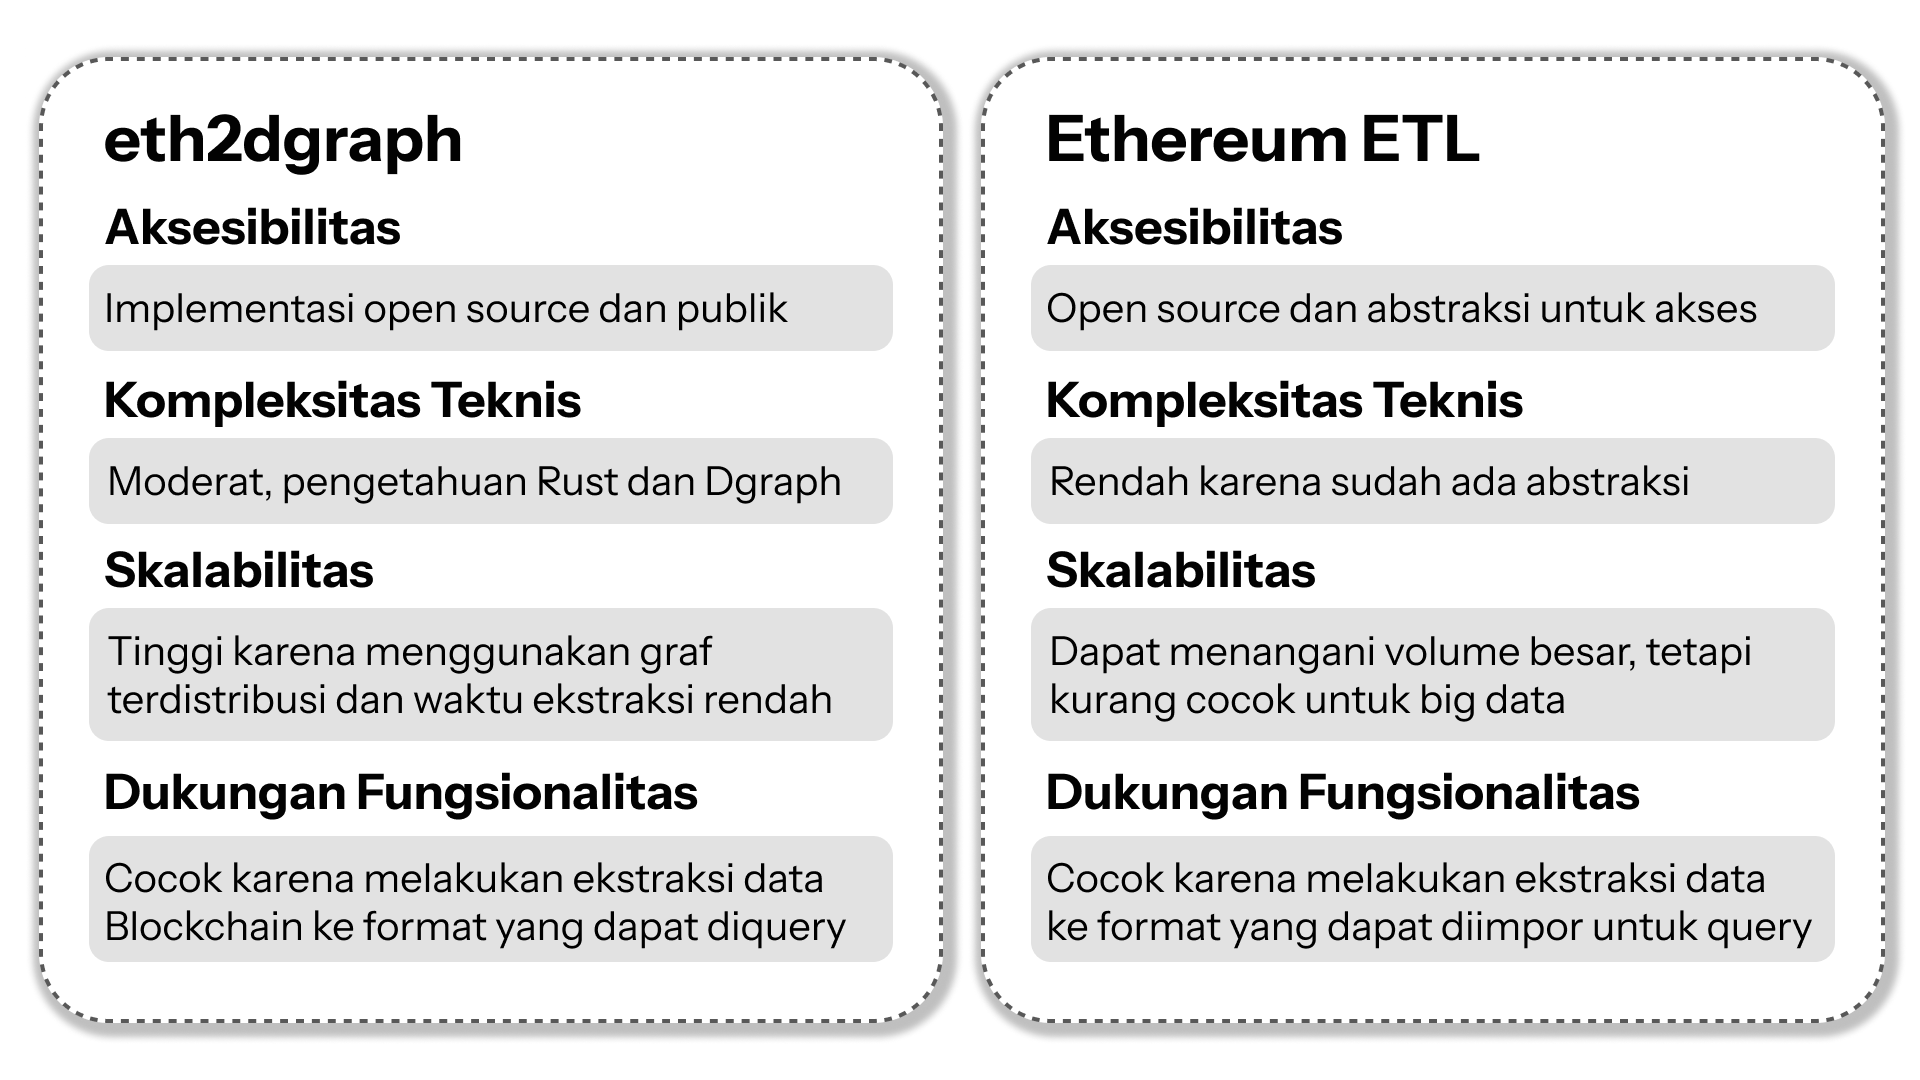
\includegraphics[width=0.9\textwidth]{resources/chapter-3/ekstraksi-1.png}
	\caption{Perbandingan alternatif ekstraksi data Smart Contracts dari Blockchain Ethereum}
	\label{image:perbandingan-ekstraksi-1}
\end{figure}

\begin{figure}[ht]
	\centering
	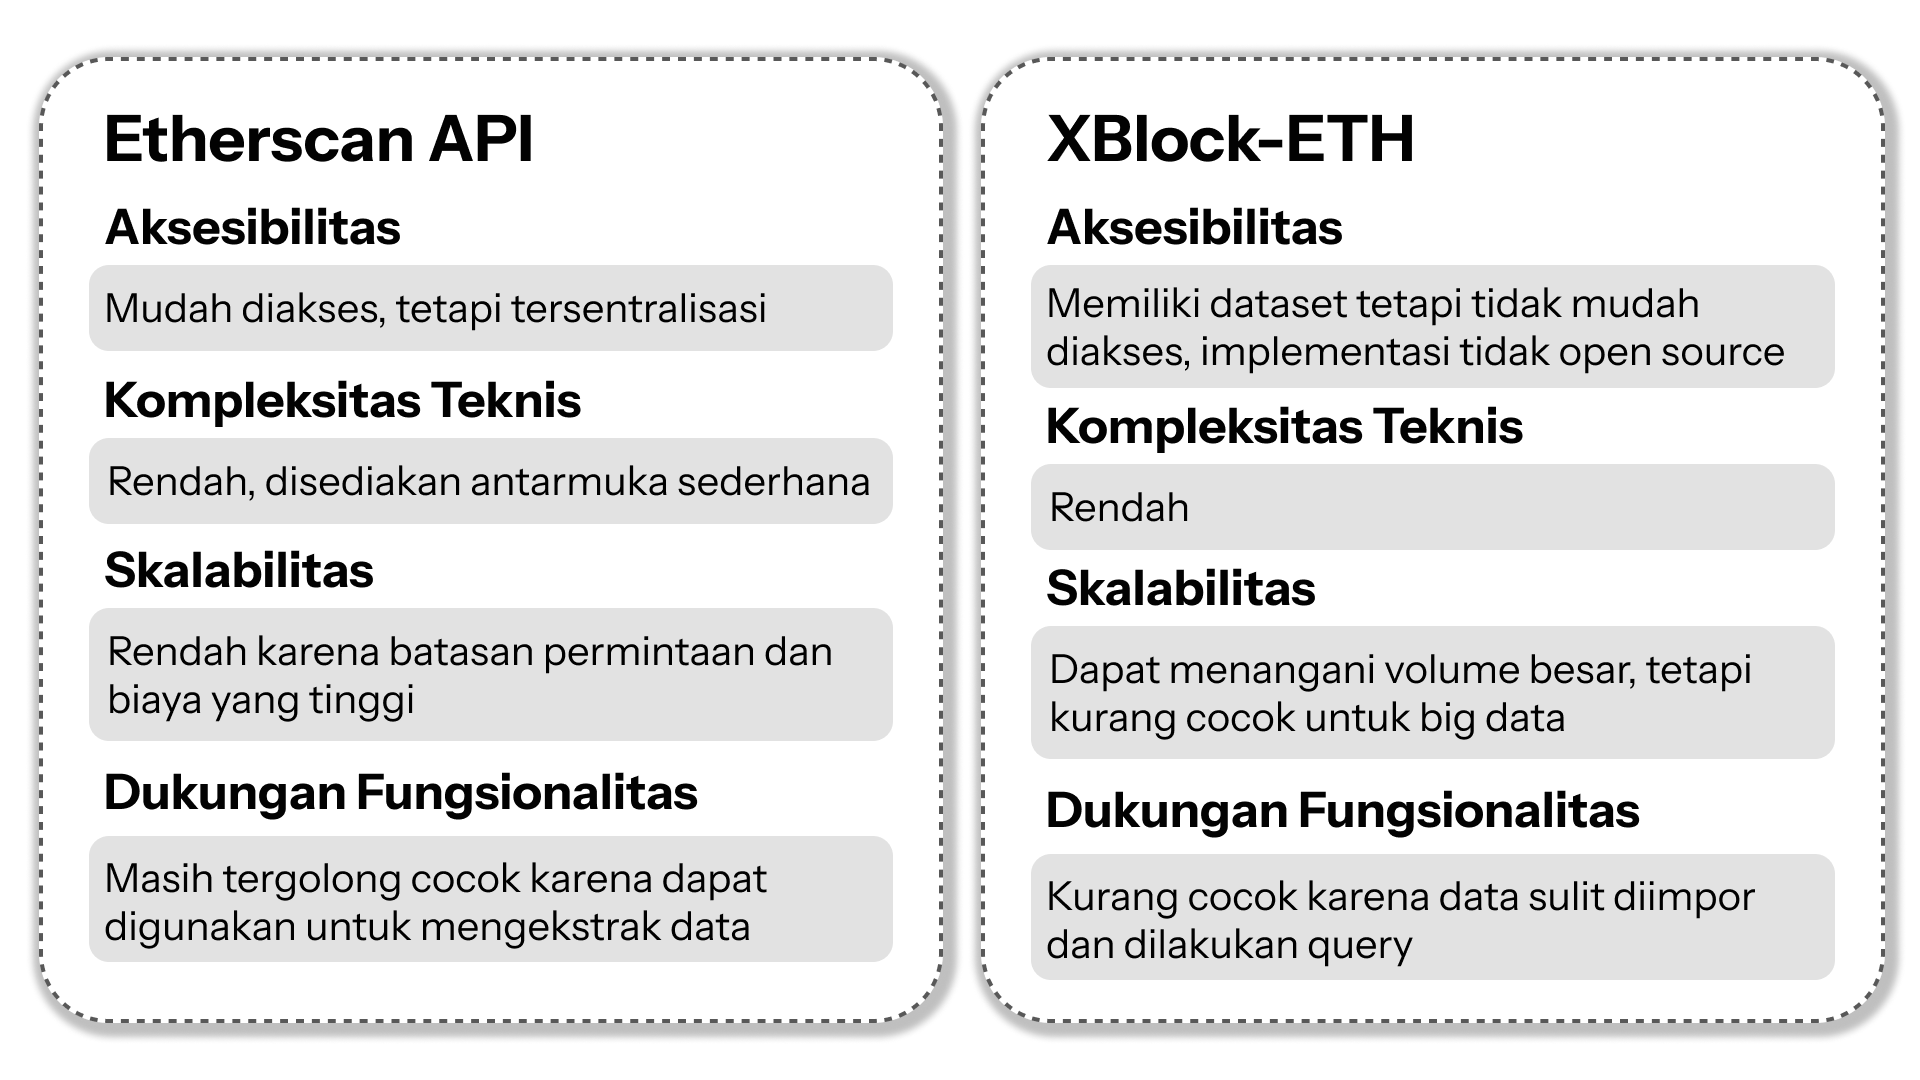
\includegraphics[width=0.9\textwidth]{resources/chapter-3/ekstraksi-2.png}
	\caption{Perbandingan alternatif ekstraksi data Smart Contracts dari Blockchain Ethereum}
	\label{image:perbandingan-ekstraksi-2}
\end{figure}

\begin{figure}[ht]
	\centering
	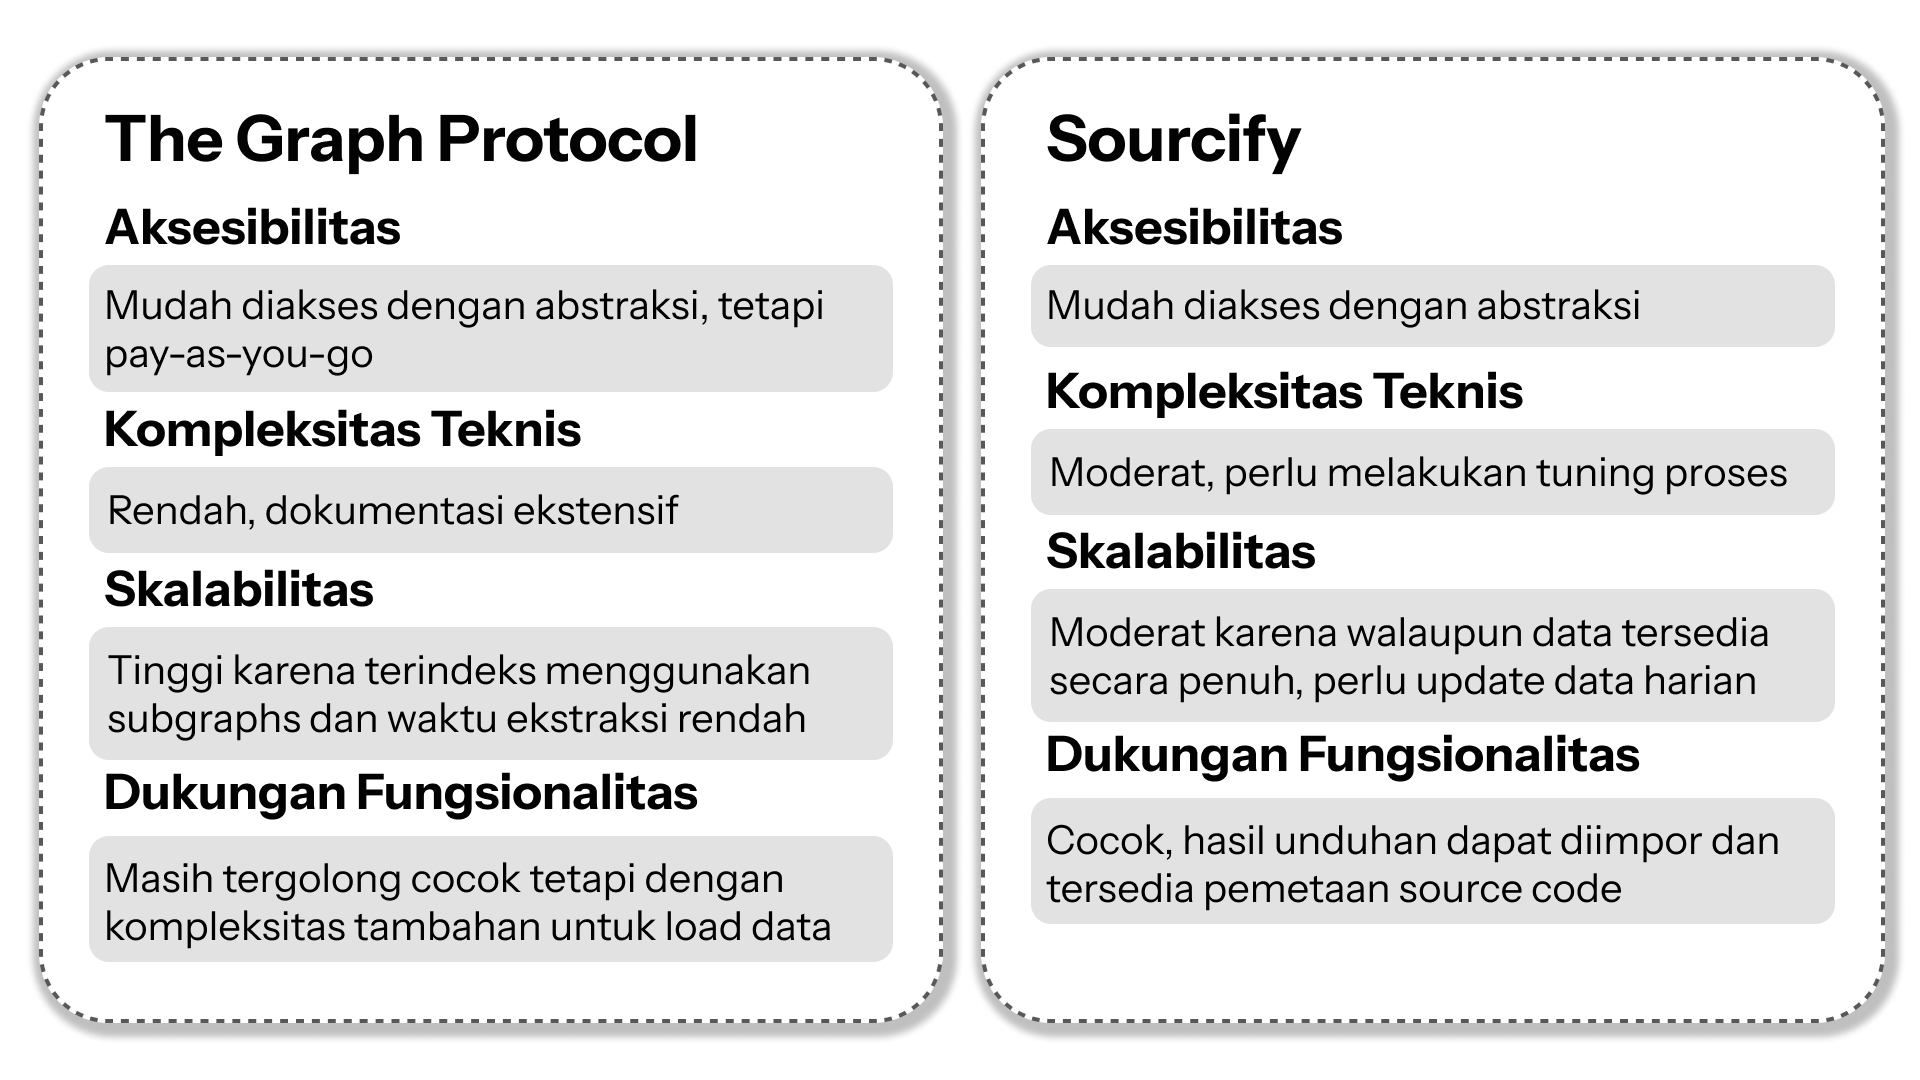
\includegraphics[width=0.9\textwidth]{resources/chapter-3/ekstraksi-3.png}
	\caption{Perbandingan alternatif ekstraksi data Smart Contracts dari Blockchain Ethereum}
	\label{image:perbandingan-ekstraksi-3}
\end{figure}

Kebutuhan pertama yang harus dipenuhi adalah ekstraksi data Smart Contracts dari Blockchain Ethereum. Proses ini mencakup pengambilan data terkait Smart Contracts, seperti ABI, bytecode, metadata, dan Verified \textit{source code}. Data ini akan digunakan untuk membangun basis data yang dapat di-query dan dianalisis lebih lanjut.

Dukungan fungsional yang diperlukan tidak hanya mencakup ekstraksi data, tetapi juga kemampuan memperoleh source code yang terverifikasi dan memetakan source code tersebut dengan deployment untuk analisis tanpa dekompilasi. Prioritas fungsionalnya adalah menghasilkan data dalam format siap pakai, memperoleh source code, dan mengaitkannya dengan deployment.

Gambar \ref{image:perbandingan-ekstraksi-1}, \ref{image:perbandingan-ekstraksi-2}, dan \ref{image:perbandingan-ekstraksi-3} menunjukkan rangkuman perbandingan berbagai alternatif ekstraksi data Smart Contracts dari Blockchain Ethereum. Secara rinci, berikut adalah analisis dari masing-masing alternatif:

\begin{enumerate}
	\item \textbf{eth2dgraph} \parencite{aimar2023extraction}: Riset ini unggul dalam mengekstrak ABI, bytecode, dan metadata yang dikonversi menjadi format graf. Implementasinya yang \textit{open source} menggunakan Rust untuk kinerja tinggi dan Dgraph untuk skalabilitas, sehingga memungkinkan query pada hubungan antar Smart Contracts di Ethereum. Pendekatan ini memerlukan \textit{node} Ethereum dan dasar pengetahuan mengenai Rust dan Dgraph. Selain ekstraksi cepat, eth2dgraph efektif dalam mengaitkan Smart Contracts Deployment dengan Verified \textit{source code} serta dapat diperluas untuk menambahkan aspek semantik.

	\item \textbf{Ethereum ETL} \parencite{ethereum_etl}: Ethereum ETL dikenal karena kemudahan penggunaan dan dokumentasinya yang lengkap, serta dukungan untuk data transaksi, blok, dan Smart Contracts. Meskipun demikian, ia tidak mendukung ekstraksi ABI, membutuhkan waktu lebih lama, dan memerlukan beberapa operasi tambahan untuk memperoleh data Smart Contracts. Hasil ekstraksinya cocok untuk basis data relasional, namun kurang ideal untuk sistem big data karena format data yang dihasilkan.

	\item \textbf{Etherscan API} \parencite{etherscan2024}: Dengan Etherscan API, pengguna dapat langsung mengekstrak data Smart Contracts beserta Verified \textit{source code} dari sumber yang terpercaya. Antarmukanya yang sederhana memudahkan akses, namun seluruh data bergantung pada Etherscan yang tersentralisasi. Batasan jumlah permintaan serta biaya penggunaan juga perlu diperhitungkan, terutama untuk ekstraksi data skala besar.

	\item \textbf{XBlock-ETH} \parencite{zheng2020xblock}: XBlock-ETH memungkinkan ekstraksi data tanpa memanfaatkan \textit{node} Ethereum, namun hasilnya disimpan dalam bentuk CSV yang memerlukan parsing tambahan dan tidak mendukung query atau indexing secara efisien. Selain itu, karena kode ekstraksinya tidak \textit{open source}, replikasi proses menjadi sulit meskipun pendekatannya cukup sederhana untuk digunakan.

	\item \textbf{The Graph Protocol} \parencite{TheGraphDocs}: The Graph menawarkan kemudahan penggunaan dengan query cepat dan infrastruktur yang terintegrasi dengan baik. Namun, model pembayaran \textit{pay-as-you-go} dapat membuat biaya ekstraksi data meningkat. Data JSON yang dihasilkan memerlukan konversi ulang ke format lain, meski flexibelnya memudahkan pengembangan lebih lanjut.

	\item \textbf{Sourcify} \parencite{sourcify_website}: Sourcify menyediakan antarmuka yang mudah untuk mengunduh dan memetakan hubungan antara \textit{source code} dan Deployment. Meskipun sudah tersedia abstraksi, ia tidak mendukung ekstraksi data kompleks seperti ABI dan bytecode. Proses pengunduhan berkala untuk memperbarui data masih perlu dioptimalkan agar lebih efisien, meskipun penggunaannya tergolong moderat.
\end{enumerate}


\subsubsection{Pemodelan, Penyimpanan, dan \textit{Indexing} Data Smart Contracts}

% jadi bahas alternatif dulu, misal yang terpilih eth2dgraph
% lalu bahas schema yang dipakainya gimana, yang base nya apa aja secara singkat, dan yang mau ditambahinnya apa, berdasarkan apa
% Jadiin dua subheading

\subsubsection{Klasifikasi Fungsional dan Semantik Smart Contracts}

\begin{figure}[ht]
	\centering
	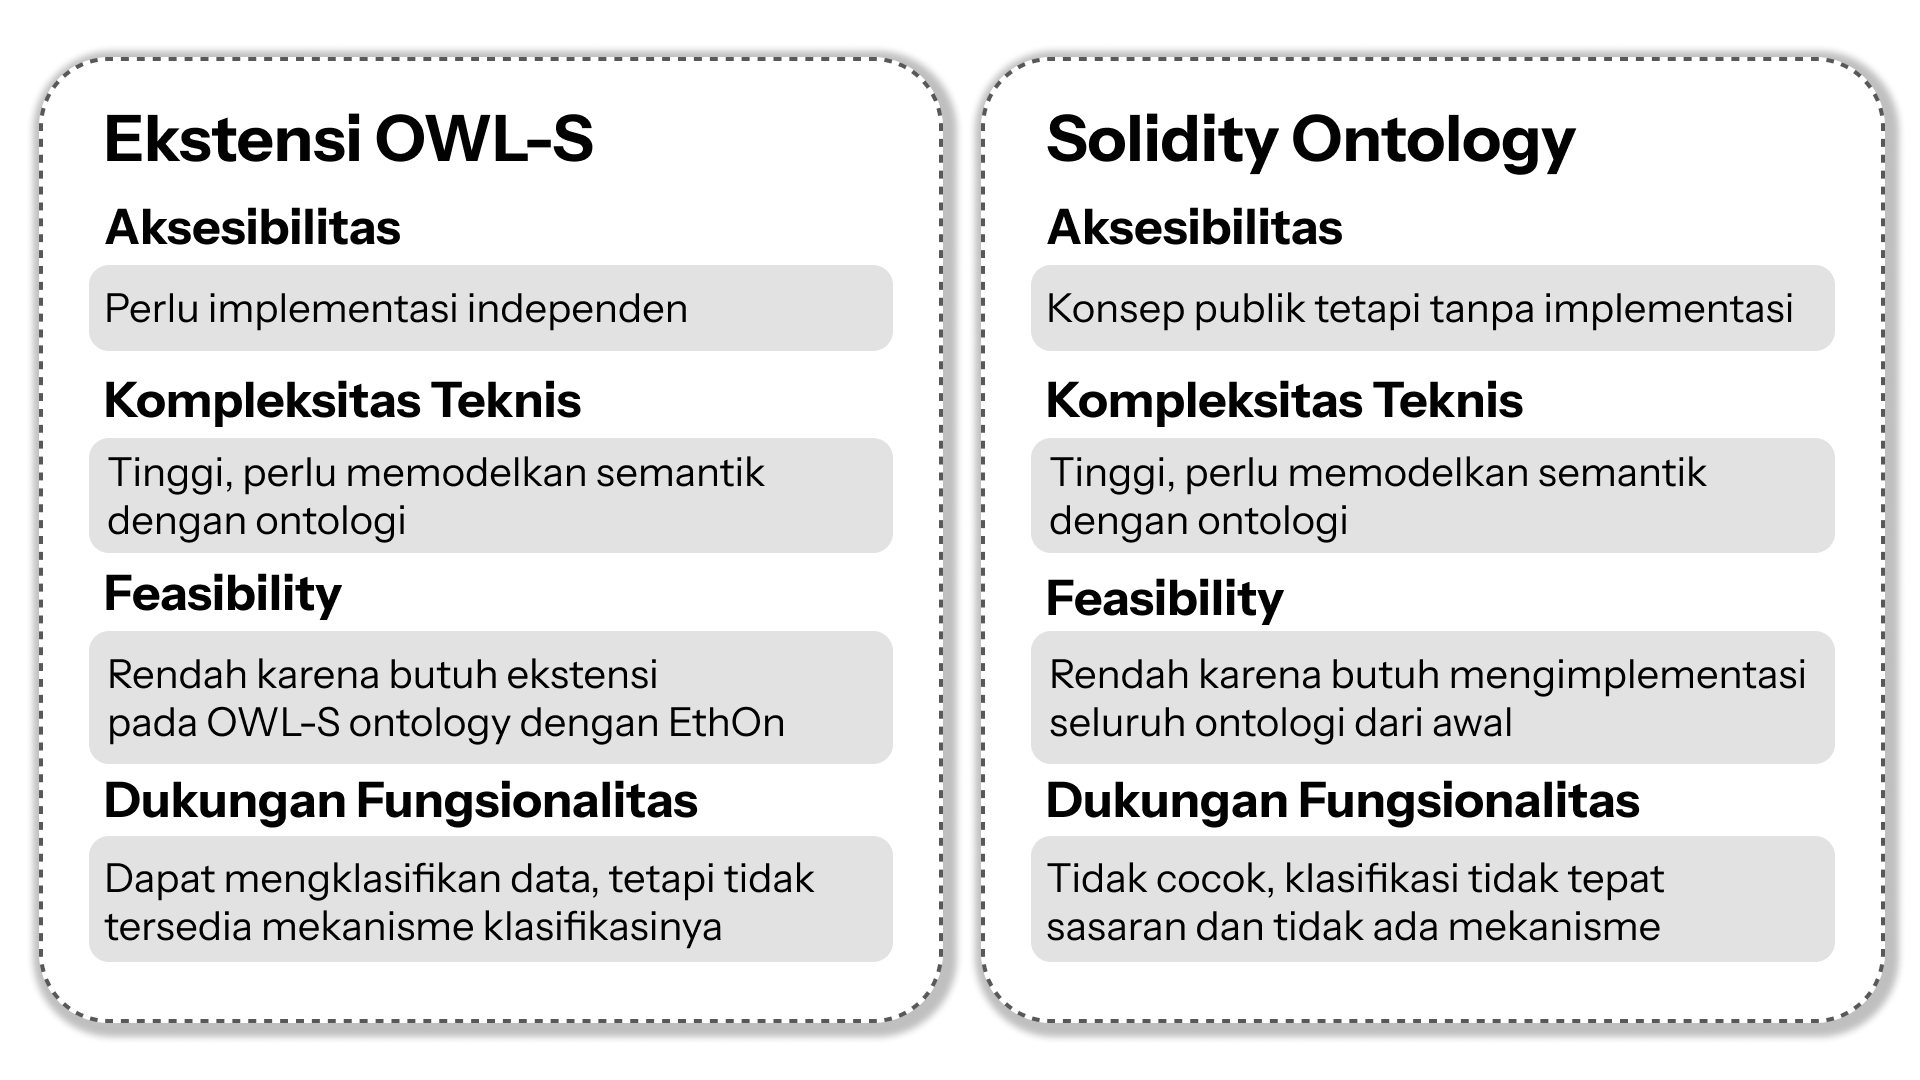
\includegraphics[width=0.9\textwidth]{resources/chapter-3/klasifikasi - 1.png}
	\caption{Perbandingan alternatif klasifikasi fungsional dan semantik Smart Contracts}
	\label{image:klasifikasi-1}
\end{figure}

\begin{figure}[ht]
	\centering
	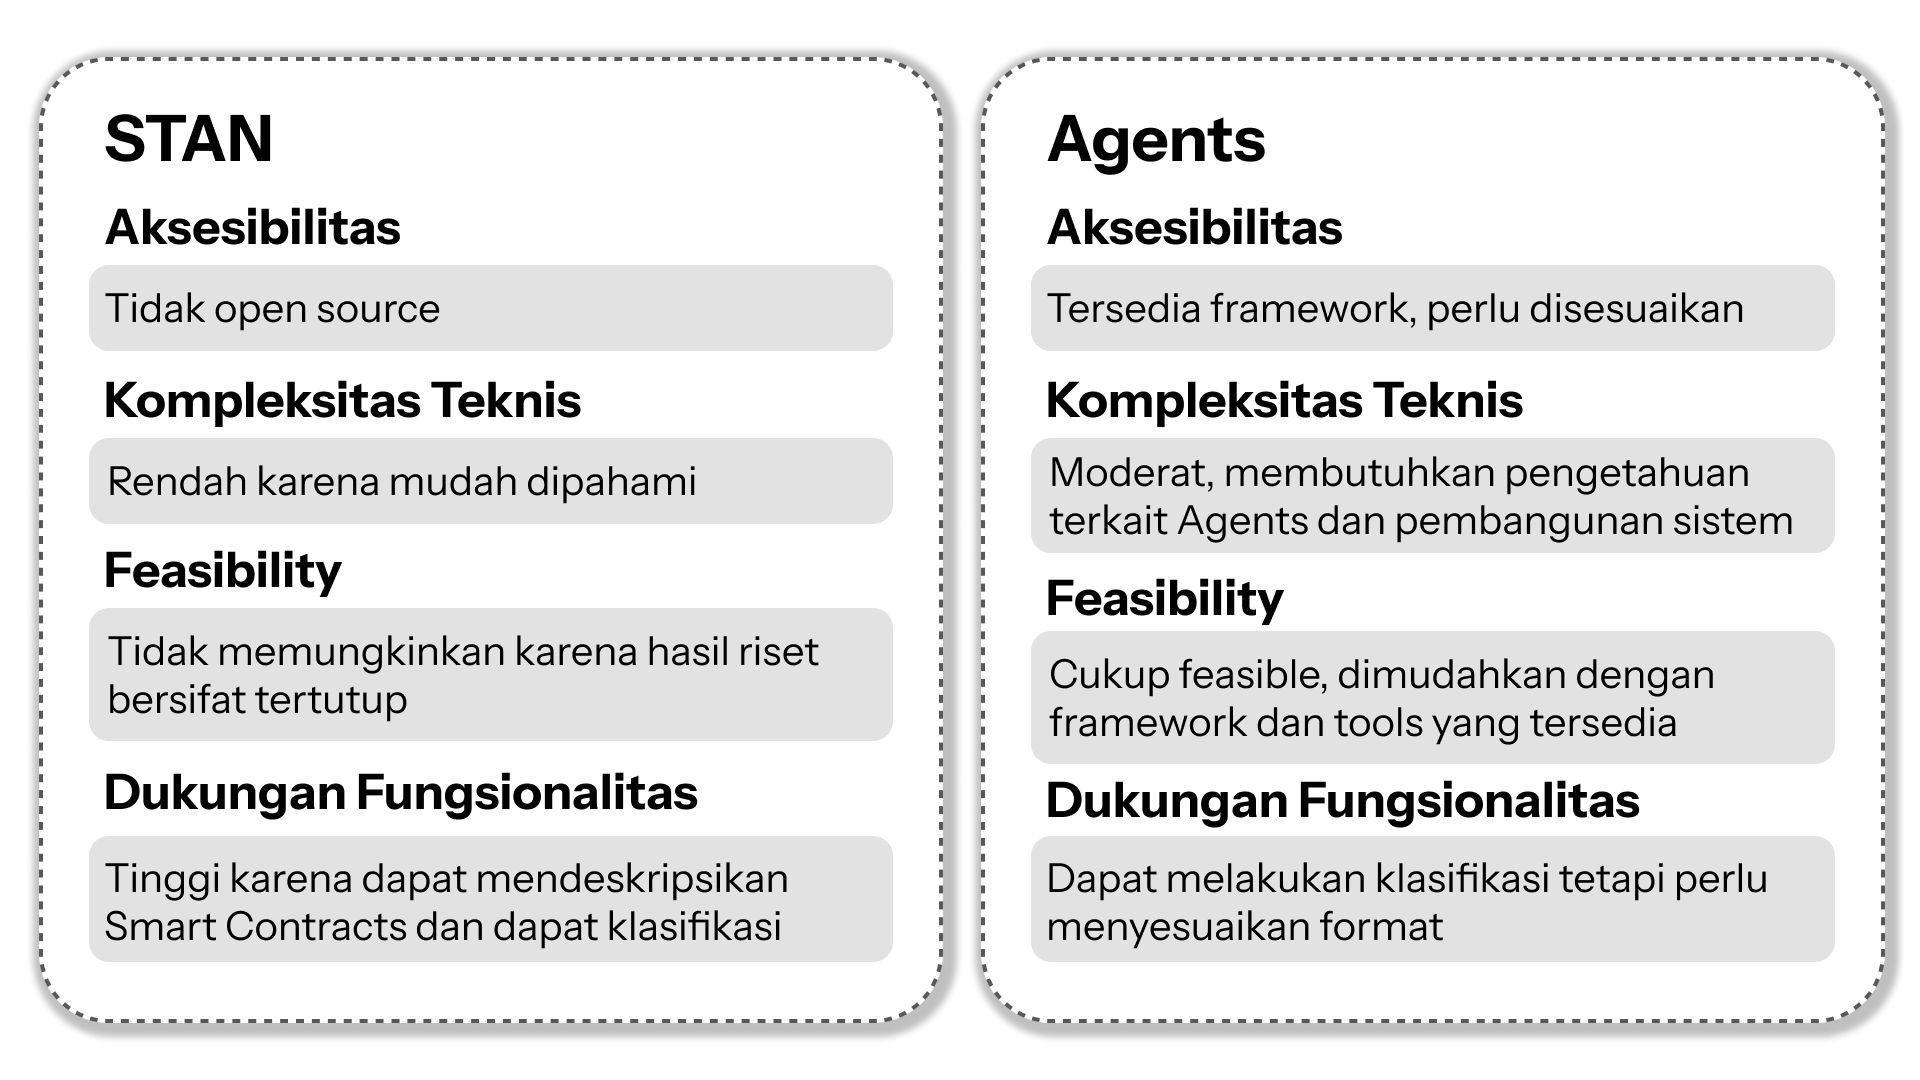
\includegraphics[width=0.9\textwidth]{resources/chapter-3/klasifikasi - 2.png}
	\caption{Perbandingan alternatif klasifikasi fungsional dan semantik Smart Contracts}
	\label{image:klasifikasi-2}
\end{figure}

\begin{figure}[ht]
	\centering
	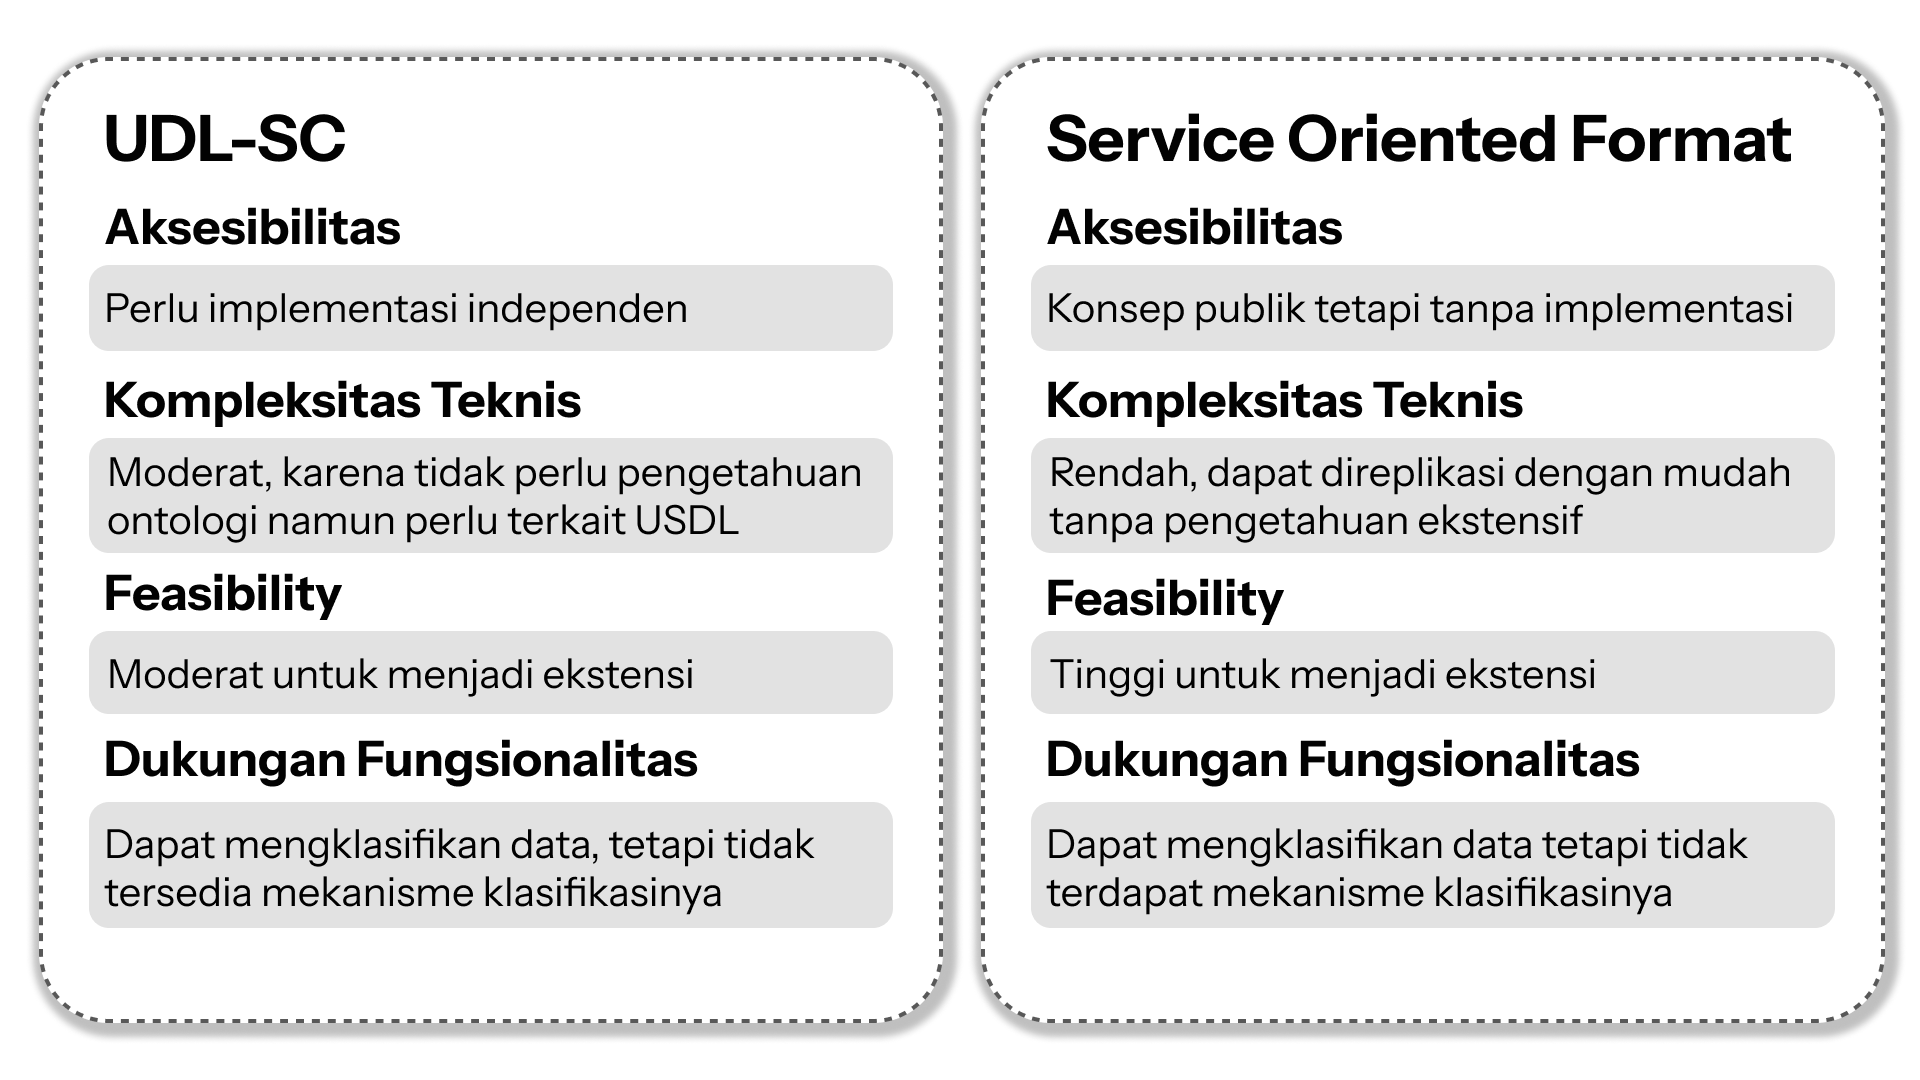
\includegraphics[width=0.9\textwidth]{resources/chapter-3/klasifikasi - 3.png}
	\caption{Perbandingan alternatif klasifikasi fungsional dan semantik Smart Contracts}
	\label{image:klasifikasi-3}
\end{figure}

\begin{figure}[ht]
	\centering
	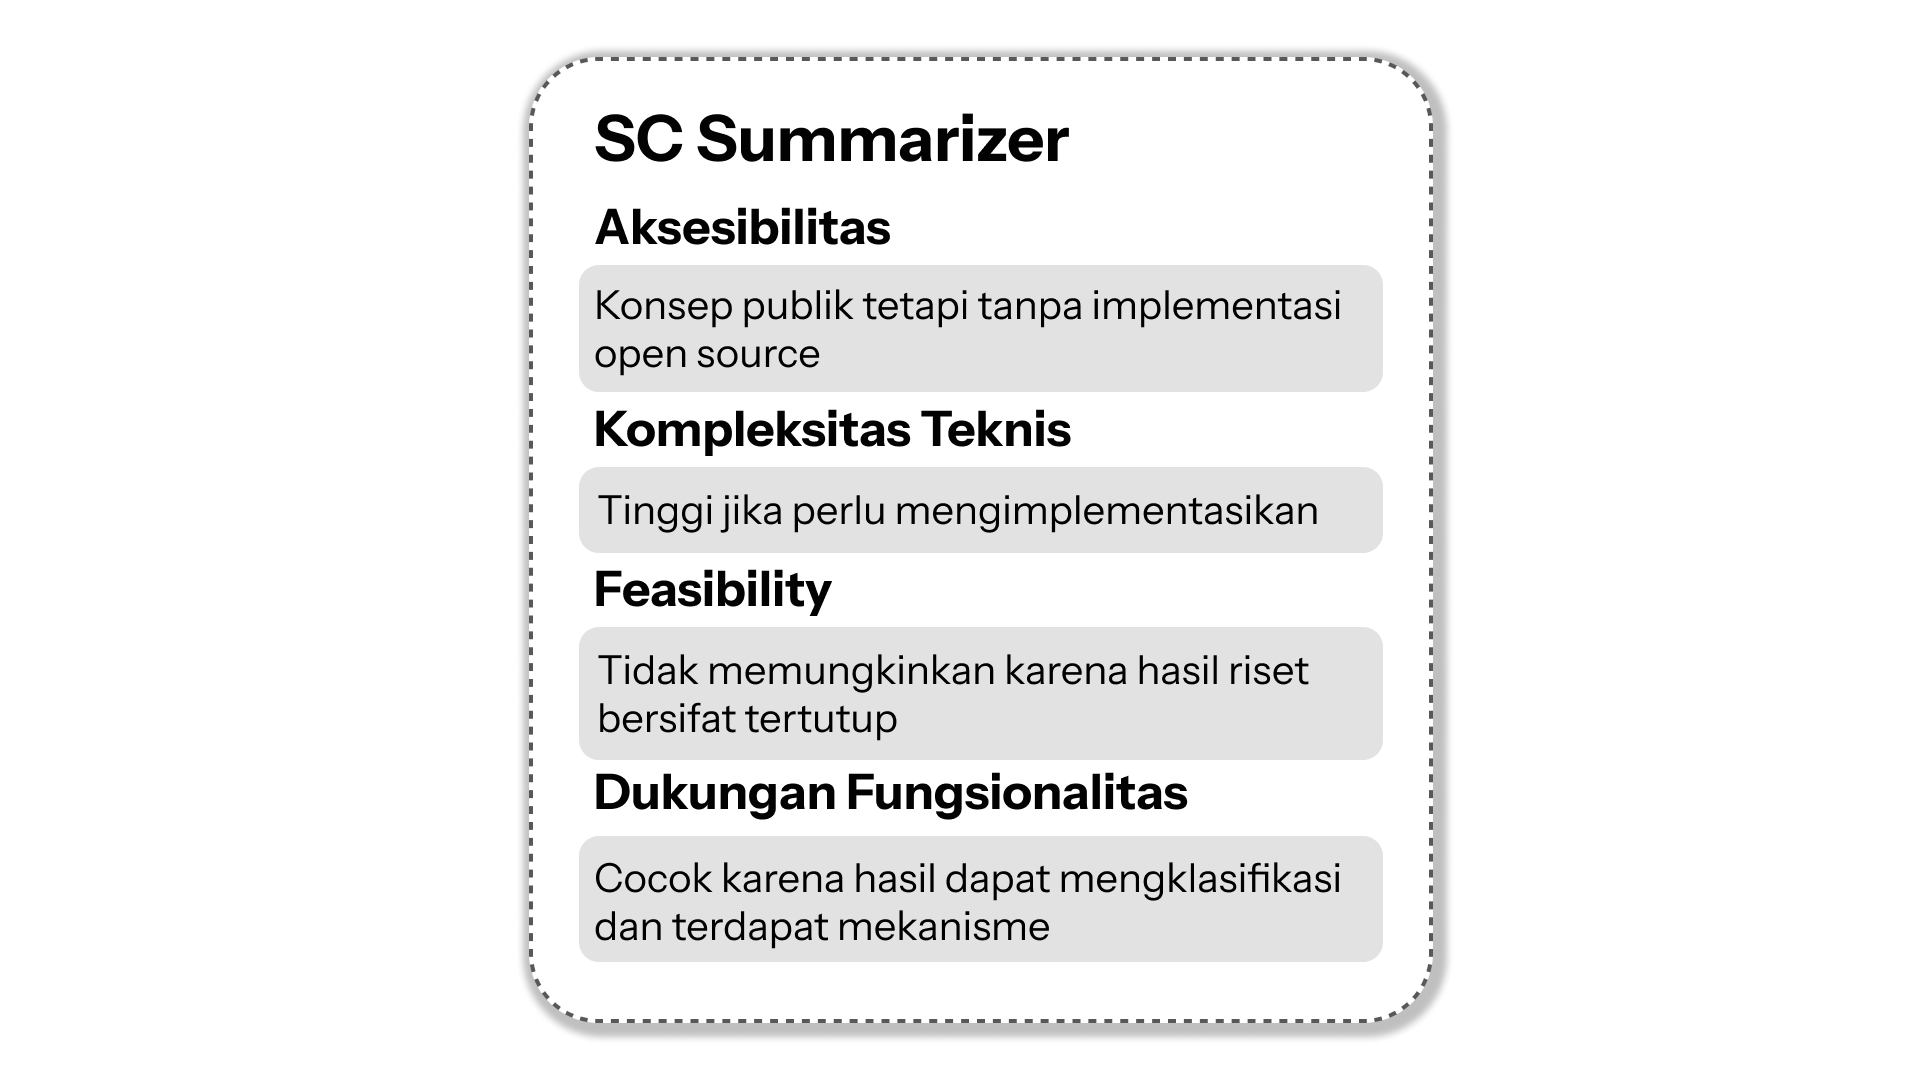
\includegraphics[width=0.9\textwidth]{resources/chapter-3/klasifikasi - 4.png}
	\caption{Perbandingan alternatif klasifikasi fungsional dan semantik Smart Contracts}
	\label{image:klasifikasi-4}
\end{figure}

Data yang sudah dimodelkan dan disimpan ke dalam sistem perlu dilakukan klasifikasi untuk memudahkan pencarian Smart Contracts berdasarkan fungsionalitas dan semantik. Terdapat berbagai alternatif untuk melakukan klasifikasi fungsional dan semantik Smart Contracts dengan berbagai pendekatan, baik dengan pemodelan ontologi, deskripsi fungsional, maupun format lainnya. Dukungan fungsional yang baik untuk klasifikasi adalah riset yang dapat melakukan klasifikasi pada data Smart Contracts dengan baik dan memberikan deskripsi atau hasil klasifikasi yang baik. Pada bagian ini, aspek skalabilitas digantikan dengan aspek \textit{feasibility}.

Gambar \ref{image:klasifikasi-1}, \ref{image:klasifikasi-2}, \ref{image:klasifikasi-3}, dan \ref{image:klasifikasi-4} menunjukkan rangkuman perbandingan berbagai alternatif klasifikasi fungsional dan semantik Smart Contracts. Secara rinci, berikut adalah analisis dari masing-masing alternatif:

\begin{enumerate}
	\item \textbf{Semantic Smart Contracts for Blockchain-based Services in the Internet of Things} \parencite{baqa2019semantic} (Bagian \ref{subsec:semantic-smart-contract-iot}): Riset ini menggunakan ekstensi pada OWL-S Service Ontology untuk melakukan klasifikasi Smart Contracts berdasarkan semantik dan fungsionalitas. Keunggulannya adalah penggunaan ontologi yang dapat di-\textit{extend} untuk menambahkan terminologi yang \textit{domain specific}. Secara aksesibilitas, riset ini bersifat \textit{public}, namun tidak memiliki implementasi \textit{open source}. Selain itu, riset ini terbatas pada \textit{scope} Internet-of-Things. Secara kompleksitas, riset ini tergolong tinggi karena memerlukan pemahaman yang mendalam tentang ontologi dan pemodelan semantik. Dalam hal dukungan fungsional, riset ini dapat memberikan deskripsi yang baik, tetapi tidak terdapat mekanisme untuk mengklasifikasikan data dengan baik.

	\item \textbf{Ontological Modeling of Smart Contracts in Solidity} \parencite{cano2021toward} (Bagian \ref{subsec:solidity-ontology}): Riset ini menerapkan ontologi pada bahasa pemrograman Solidity. Ontologi ini digunakan untuk mendeskripsikan elemen-elemen dalam Smart Contracts, seperti fungsi, variabel, dan struktur data. Secara aksesibilitas, riset ini bersifat publik, dengan ontologi yang dihasilkan dapat diterapkan. Namun, implementasi ontologi pada riset ini terbatas pada sintaks dan semantik dari kode bahasa pemrograman Solidity sendiri dibandingkan Smart Contracts secara keseluruhan. Secara kompleksitas, riset ini tergolong tinggi karena memerlukan pemahaman yang mendalam tentang ontologi dan pemodelan semantik, dan memerlukan proses klasifikasi yang ekstensif untuk memetakan data dengan ontologi yang dihasilkan. Dalam hal dukungan fungsional, riset ini tidak sesuai dengan kebutuhan sistem, yaitu memodelkan fungsionalitas dari Smart Contract, bukan aspek sintaks bahasa pemrograman Soliditynya, dan tidak terdapat mekanisme untuk mengklasifikasikan data dengan baik.

	\item \textbf{STAN} \parencite{stan} (Bagian \ref{subsec:stan}): STAN adalah sebuah sistem untuk memberikan deskripsi terhadap bytecodes dari Smart Contracts. Secara aksesibilitas, STAN tidak bersifat \textit{open source}, sehingga tidak tersedia implementasinya untuk melakukan replikasi. Secara kompleksitas, STAN tergolong rendah karena abstraksi yang sudah diberikan untuk menghasilkan deskripsi. Riset STAN ini juga belum menginkorporasikan teknologi seperti Artificial Intelligence (AI) untuk melakukan klasifikasi. Dalam hal dukungan fungsional, STAN dapat membantu mengklasifikasikan Smart Contracts berdasarkan deskripsi yang dihasilkan.

	% \item \textbf{Agents} (Bagian \ref{sec:agents}): Alternatif untuk melakukan klasifikasi Smart Contracts adalah menggunakan AI Agents yang dapat melakukan dekomposisi tasks yang kompleks menjadi sub-tasks yang lebih sederhana. Dengan menggunakan AI Agents, klasifikasi Smart Contracts dapat dilakukan dengan lebih menyeluruh dan efisien karena dapat memperhitungkan berbagai aspek yang ada pada Smart Contracts. Secara aksesibilitas, sudah banyak \textit{framework} dan \textit{tools} yang tersedia untuk membangun sebuah sistem berbasis AI Agents (Agentic AI). Namun, perlu dilakukan pembangunan secara independen karena tidak ada sistem yang secara langsung memberikan fungsionalitas yang sesuai. Secara kompleksitas, penggunaan AI Agents tergolong moderat karena memerlukan pengetahuan terkait AI dan membuat sistem berbasis AI Agents. Secara \textit{feasibility}, pembangunan sistem berbasis agents cukup \textit{feasible} dengan penggunaan \textit{framework} dan \textit{tools} yang baik. Dukungan fungsional yang diberikan oleh sistem dengan AI Agents tergolong baik karena dapat disesuaikan dan melakukan pekerjaan kompleks secara otonom, tetapi perlu menggunakan format yang disesuaikan untuk mendeskripsikan data.
	      % menggunakan agents yang dimasukkin source code, dengan break down step by step

	\item \textbf{LLM Classification} (Bagian \ref{sec:llms}): Penggunaan LLM untuk melakukan klasifikasi Smart Contracts dengan menghasilkan deskripsi dan mengklasifikasikan berdasarkan deskripsi yang dihasilkan. Dengan memanfaatkan kemampuan LLM dalam memahami konteks dan semantik, diharapkan klasifikasi dapat dilakukan dengan lebih akurat dan efisien. Secara aksesibilitas, LLMs seperti GPT-4 dan Llama-3 sudah tersedia untuk digunakan, baik melalui API maupun model yang dapat diunduh. Secara kompleksitas, penggunaan LLMs tergolong rendah karena hanya memerlukan pengetahuan dasar tentang pemrograman dan penggunaan API. Secara \textit{feasibility}, sistem ini \textit{feasible} untuk diimplementasikan dengan infrastruktur yang ada. Dalam hal dukungan fungsional, LLMs dapat memberikan deskripsi yang baik dan melakukan klasifikasi Smart Contracts dengan baik, tetapi perlu diperhatikan bahwa LLMs tidak selalu memberikan hasil yang konsisten.

	\item \textbf{Uniform Description Language for Smart Contracts} \parencite{udlsc} (Bagian \ref{subsec:uniform-description-language}): Riset ini mengusulkan sebuah bahasa deskripsi ekstensi dari USDL untuk Smart Contracts. Secara aksesibilitas, hasil dari riset ini bersifat \textit{public}, namun perlu melakukan replikasi untuk mendapatkan hasil yang didapatkan dari riset. Secara kompleksitas, riset ini tergolong moderat karena walaupun tidak memerlukan pengetahuan yang mendalam terkait ontologi, perlu memahami terkait USDL dan implementasi ekstensi dari USDL. Secara skalabilitas, riset ini tergolong baik karena dapat digunakan sebagai ekstensi data tanpa masalah. Dalam hal dukungan fungsional, riset ini kurang baik karena tidak terdapat mekanisme untuk mengklasifikasikan data dengan baik, tetapi dapat digunakan untuk mendeskripsikan data Smart Contracts dengan baik.

	\item \textbf{Service Oriented Format Descriptor} \parencite{guida2019supporting} (Bagian \ref{subsec:supporting-reuse-smart-contracts}): Riset ini mengusulkan sebuah format deskripsi untuk Smart Contracts dengan pendekatan Service. Riset ini juga mengusulkan sebuah Service Registry dan Contract Editor berbasis visual yang mengkomplemen format deskripsi yang diusulkan. Format deskripsi ini dapat digunakan dan digabungkan dengan sistem lain, sedangkan Service Registry dan Contract Editor kurang fleksibel untuk diintegrasikan dengan sistem lain. Secara aksesibilitas, hasil dari riset ini bersifat \textit{public} dan \textit{open source}, sehingga dapat digunakan untuk melakukan replikasi. Secara kompleksitas, format yang dihasilkan oleh riset ini tergolong rendah karena tidak memerlukan pengetahuan yang mendalam dan dapat langsung dijadikan ekstensi ke format lain. Dalam hal dukungan fungsional, riset ini dapat mengakomodasi deskripsi Smart Contracts dengan baik, tetapi tidak ada mekanisme untuk melakukan klasifikasi data dengan baik.

	\item \textbf{Smart Contract Summarizer} \parencite{zhang2021smart} (Bagian \ref{subsec:smart-contract-solidity-summary}): Riset ini mengusulkan sebuah sistem untuk menghasilkan ringkasan dan anotasi dari Smart Contracts, terutama dalam bahasa Solidity. Sistem ini menggunakan teknik NLG (Natural Language Generation) dengan pendekatan berbasis \textit{transformer} untuk menghasilkan ringkasan yang lebih baik dibandingkan dengan metode berbasis template sebelumnya. Secara aksesibilitas, konsep dari riset ini bersifat \textit{public}, namun tidak memiliki implementasi \textit{open source}. Secara kompleksitas, jika perlu mengimplementasikan dari awal, riset ini tergolong tinggi karena memerlukan pengetahuan yang mendalam terkait NLP dan pemodelan semantik. Secara skalabilitas, sistem ini tidak diketahui untuk kinerja menangani data yang banyak. Dalam hal dukungan fungsional, riset ini dapat membantu mengklasifikasikan Smart Contracts berdasarkan ringkasan yang dihasilkan dengan mekanisme yang digunakan.

\end{enumerate}


\subsubsection{Pencarian dan Rekomendasi Smart Contracts}

% ini LLM, terus pake langchain?? (iya si harusnya (recheck obsidian pls))

\subsubsection{Interaksi Pengguna dengan Sistem}


\subsubsection{Kesimpulan Pemilihan Alternatif}

\begin{figure}[ht]
	\centering
	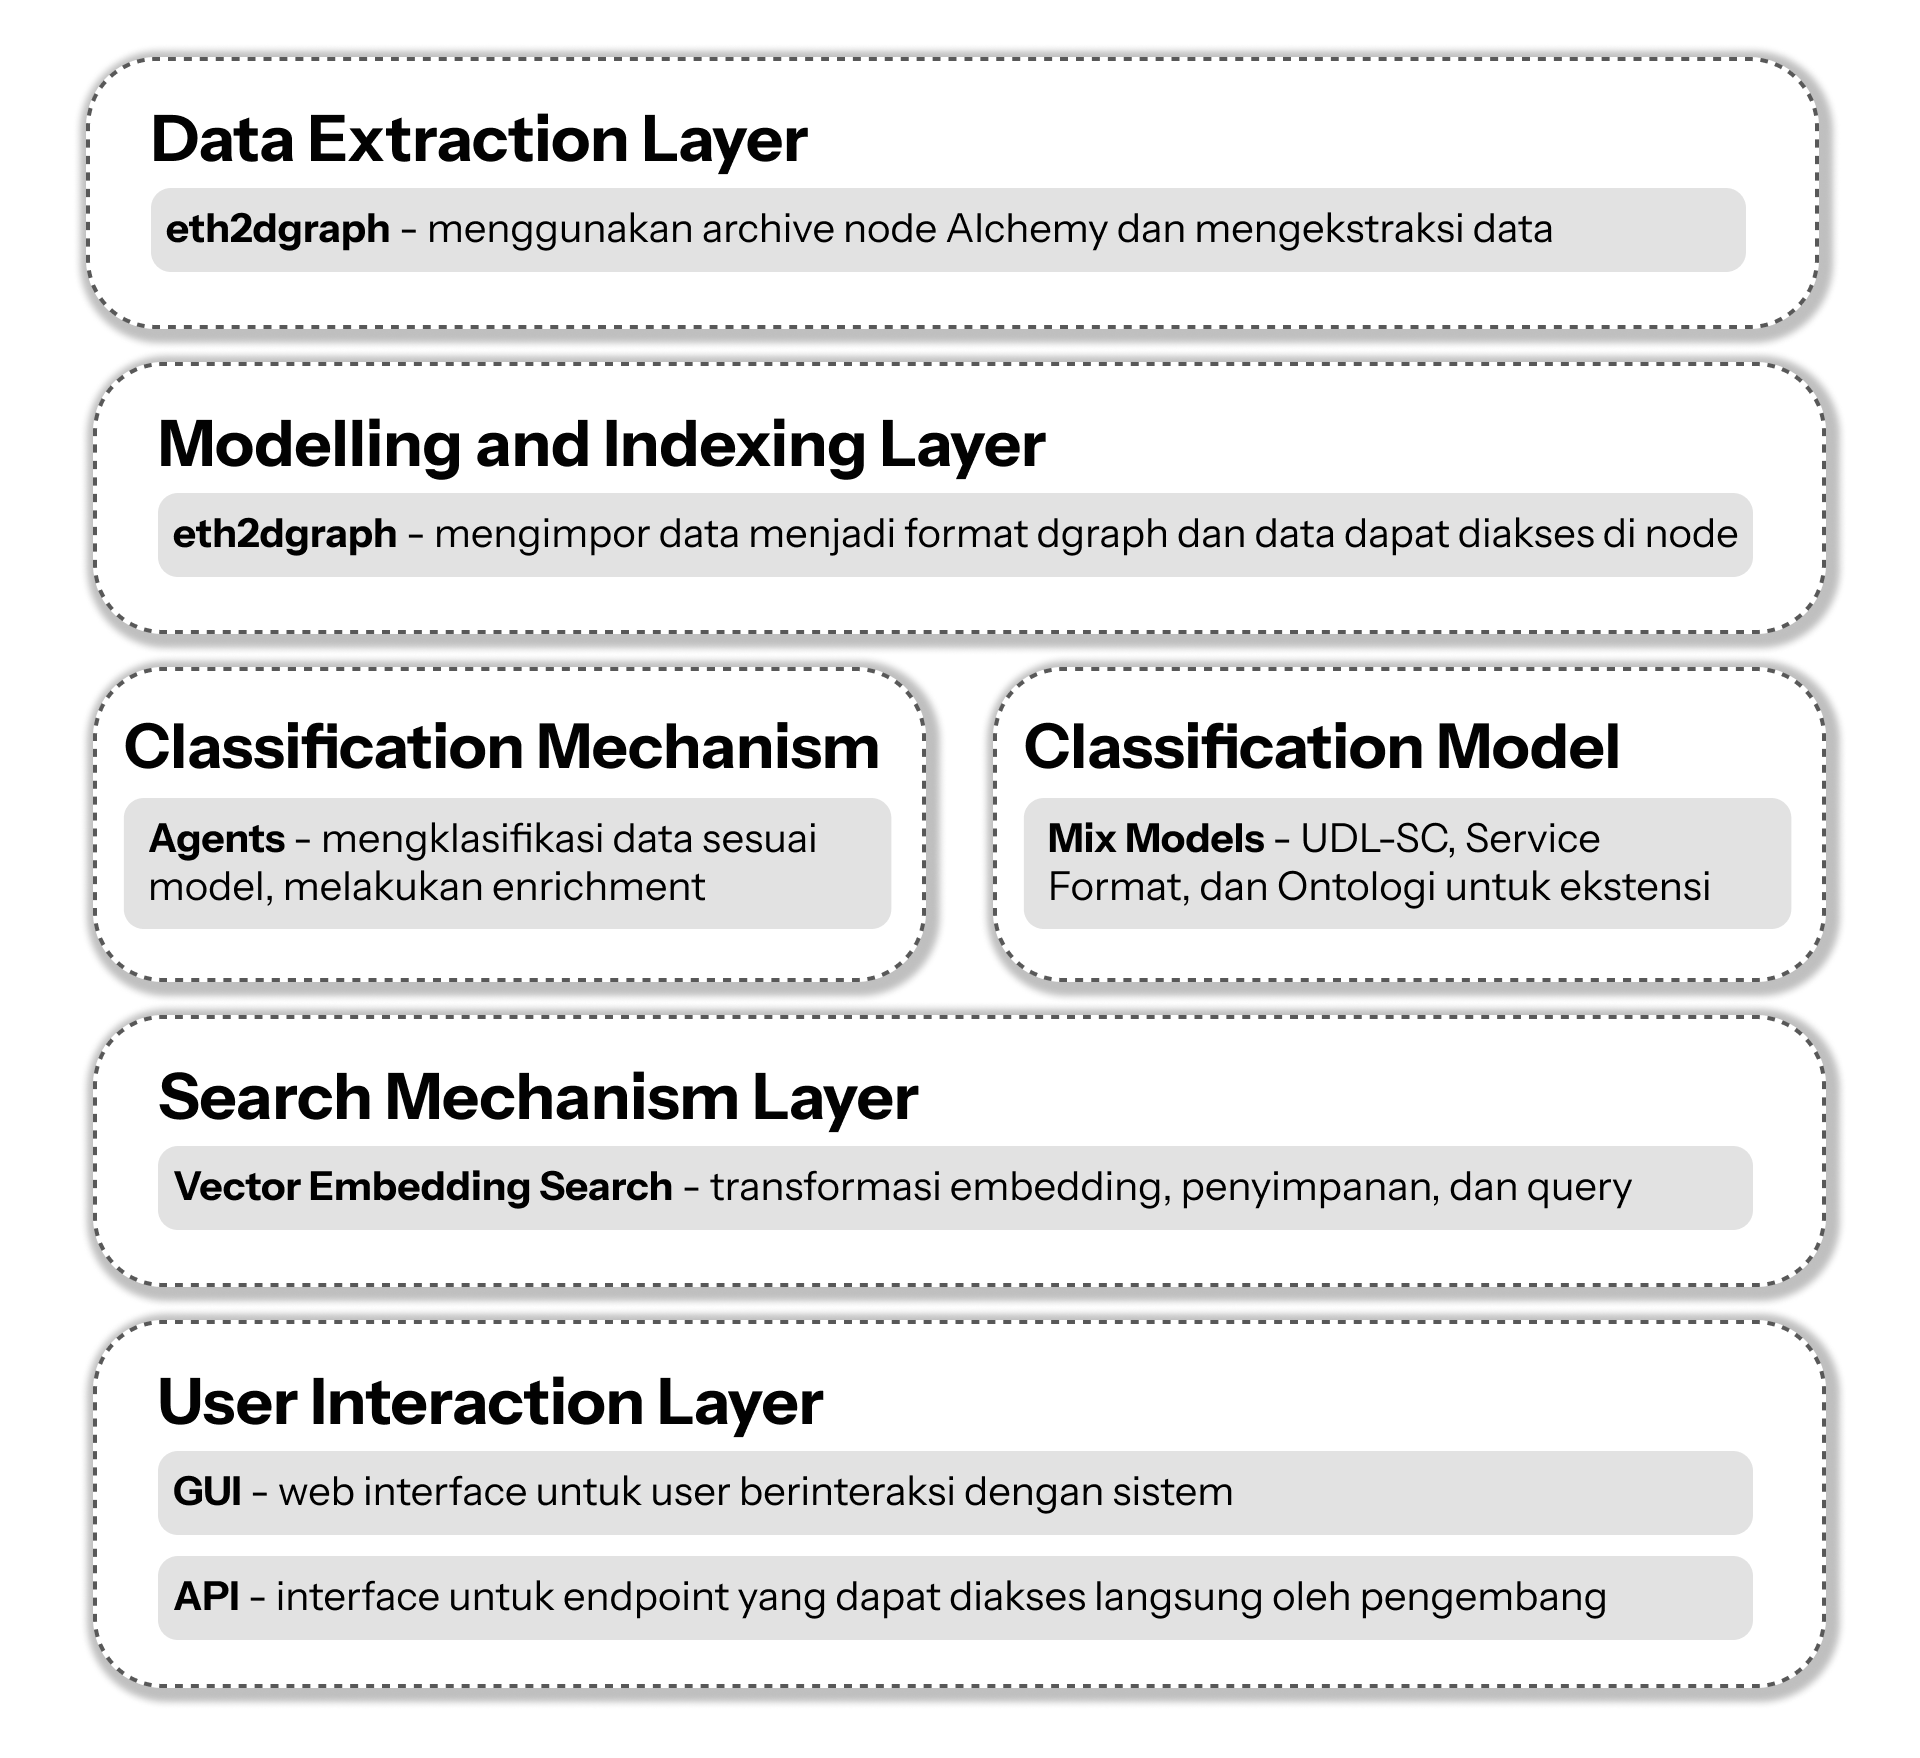
\includegraphics[width=0.7\textwidth]{resources/chapter-3/hasil-pemilihan.png}
	\caption{Kesimpulan pemilihan alternatif}
	\label{image:layer-architecture}
\end{figure}

Berdasarkan analisis dari alternatif-alternatif yang dibahas pada bagian \ref{subsec:analisis-alternatif-solusi}, dapat disimpulkan bahwa alternatif yang dipilih untuk membangun sistem adalah sebagai berikut:

\begin{enumerate}
	\item \textbf{Ekstraksi data Smart Contracts dari Blockchain Ethereum}: Alternatif yang dipilih adalah \textit{eth2dgraph} \parencite{aimar2023extraction}, karena memiliki aksesibilitas yang baik, bersifat \textit{open source}, memiliki kecepatan ekstraksi yang tinggi, dan juga menyediakan infrastruktur lengkap sampai pada penyimpanan data dalam format Distributed Graph Database.
	\item \textbf{Pemodelan, penyimpanan, dan \textit{indexing} data Smart Contracts}: Alternatif yang dipilih adalah \textit{eth2dgraph} \parencite{aimar2023extraction}, karena memiliki kemampuan skalabilitas tinggi dan dapat melakukan query dengan efisien. Selain itu, Dgraph juga memiliki kemampuan untuk melakukan \textit{indexing} data dengan baik.
	\item \textbf{Klasifikasi fungsional dan semantik Smart Contracts}: Alternatif yang dipilih untuk mekanisme klasifikasi adalah LLM Classification, karena memliki kemampuan kustomisasi yang baik untuk mendeskripsikan dan mengklasifikasi Smart Contracts. Model yang akan digunakan adalah model tekstual, yaitu penjelasan fungsionalitas Smart Contracts dalam bahasa alami, dengan kombinasi dengan konsep ontologi dalam bentuk metadata untuk pengklasifikasian. Metadata dengan konsep ontologi ini akan membuat atribut data lebih mudah untuk diekstrak menjadi sebuah ontologi.
	\item \textbf{Pencarian dan rekomendasi Smart Contracts}: Alternatif yang dipilih untuk mekanisme pencarian awal adalah alternatif Vector Embedding Search, karena simplisitas yang ditawarkan dan tidak ada redundansi \textit{layer}. Alternatif yang dapat dikonsiderasikan untuk pengembangan berikutnya, terutama jika dikembangkan sebuah fitur untuk berinteraksi dengan sistem yang lebih kompleks adalah alternatif \textit{Retrieval-Augmented Generation (RAG)}, karena dapat mengakomodasi interaksi yang lebih kompleks.
	\item \textbf{Interaksi pengguna dengan sistem}: API dan GUI akan diimplementasikan untuk interaksi pengguna dengan sistem karena dapat memberikan fleksibilitas dan kemudahan bagi pengguna. Sehingga, pengguna dapat melakukan pencarian Smart Contracts dengan cara yang sesuai dengan kebutuhan mereka.
\end{enumerate}

% Untuk mengatasi permasalahan pemilihan Smart Contracts yang tepat dan mengurangi redundansi Smart Contracts di Blockchain, solusi yang diusulkan adalah sebuah sistem pencarian Smart Contracts yang dapat memberikan hasil berdasarkan fungsionalitas Smart Contracts. Sistem akan dibangun dengan memanfaatkan berbagai teknologi dan riset yang sudah ada, yang melakukan \textit{indexing} maupun modeling yang menjadikan Smart Contracts \textit{discoverable} untuk mengefisiensikan pengembangan.

% Beberapa riset yang dilakukan peninjauan untuk digunakan sebagai basis adalah riset oleh \cite{third2017linked}, \cite{aimar2023extraction}, \cite{baqa2019semantic}, \cite{cano2021toward}. Peninjauan didasari dengan beberapa aspek yaitu aksesibilitas dari hasil riset, kompleksitas teknis, skalabilitas, dan dukungan fungsional untuk mencapai tujuan utama.

% % Masukin diagram yang dibuat di ppt

% % preliminary analysis

% % gambaran solusi

% % menjelaskan secara lebih detail latar belakang dan masalah yang menjadi dasar munculnya topik TA ini, intinya kita coba lihat & analisis gapnya 
% % gap analysis
% % kaitan antara sistem yang dikembangkan dengan yang terkait -> apa kelebihannya? atau apa kekurangan dari aplikasi lain? emang belum terpenuhi? apa yang belum terpenuhi?
% % posisi sistem yang dikembangkan terhadap sistem yang lebih besar

% % PLACEHOLDER
% \subsubsection{Semantic Indexing with Linked Data \parencite{third2017linked}}

% Riset ini menerapkan indeks semantik pada data Blockchain menggunakan Linked Data dengan keunggulan penggunaan ontology BLONDiE dan MSM untuk mendeskripsikan semantik Smart Contracts dan fokus pada aspek \textit{discoverability}. Secara aksesibilitas, konsep riset ini \textit{public}, namun tanpa implementasi \textit{open source}. Implementasinya kompleks karena memerlukan pemetaan ontology ekstensif dan RDF triple generation, tanpa dukungan \textit{tools} atau \textit{framework}. Skalabilitas riset ini terbatas karena bergantung pada RDF-based Linked Data, yang kurang cocok untuk data Blockchain besar.

% \subsubsection{eth2dgraph \parencite{aimar2023extraction}}

% Riset ini berfokus pada ekstraksi, \textit{indexing}, dan penyimpanan data Ethereum berbasis Distributed Graph. Keunggulannya adalah penggunaan ekstraksi ABI, bytecode, dan metadata yang dapat diubah menjadi format berbasis graf, serta implementasinya yang \textit{open source} dan \textit{public}. Menggunakan Rust untuk performa tinggi dan Dgraph untuk skalabilitas, riset ini dapat melakukan query pada hubungan Smart Contracts di Ethereum. Kompleksitasnya moderat karena memerlukan pengetahuan dasar tentang Rust dan Dgraph, namun dapat diperluas untuk menambahkan aspek semantik. Skalabilitasnya tinggi berkat kinerja Dgraph.

% \subsubsection{Alternatif Lainnya}

% Kedua riset alternatif lainnya oleh \cite{baqa2019semantic} dan \cite{cano2021toward} tidak dapat dipilih karena \textit{domain} yang terlalu spesifik, ditambah dengan implementasi yang tidak bersifat \textit{open source} dan \textit{public}.

% \subsubsection{Hasil Analisis}

% Setelah melakukan analisis dari alternatif yang ada, diputuskan untuk menggunakan riset oleh \cite{aimar2023extraction}, karena memiliki implementasi yang \textit{open source}, yang mempermudah ekstraksi dan \textit{indexing} data menjadi Graph Database, sehingga tidak perlu membuat RDF Triples ada model ontology dari awal. Distributed Graph Database juga memiliki skalabilitas yang baik untuk data yang banyak pada Blockchain Ethereum. eth2dgraph juga memiliki kemampuan ekstensibilitas yang baik dalam \textit{domain} yang lebih umum, sehingga lebih mudah diimplementasikan sebagai fondasi dari sistem keseluruhan. 

% \subsubsection{Rancangan Solusi}

% Dengan penggunaan eth2dgraph sebagai fondasi dari sistem pencarian Smart Contract, berikut merupakan ajuan rancangan dari sistem:

% \begin{enumerate}
%   \item Layer 1: Blockchain Data Extraction (eth2dgraph) \newline Ekstraksi data Blockchain Ethereum menjadi Dgraph
%   \item Layer 2: Semantic Indexing and Enrichment \newline \textit{Mapping} data hasil ekstraksi kepada sebuah ontology seperti BLONDiE atau EthOn, pelabelan fungsional Smart Contracts, dan Version Control
%   \item Layer 3: Query and Discovery System \newline Sebuah Search Engine menggunakan GraphQL Queries diatas Dgraph Database yang memperkenalkan pencarian berbasis semantik
%   \item Layer 4: User Interaction Layer \newline Sebuah \textit{dashboard} atau API untuk pengembang melakukan pencarian Smart Contracts berdasarkan fungsionalitas, metadata, atau relasi, membandingkan Smart Contracts yang serupa, dan melakukan \textit{export} atau \textit{reuse} dari Smart Contract 
% \end{enumerate}


\subsection{Analisis Kebutuhan Sistem}

% bingung nulis apa lagi disini
Pada bagian \ref{subsec:analisis-alternatif-solusi}, telah disimpulkan pilihan alternatif yang akan digunakan dalam membangun sistem. Alternatif-alternatif solusi yang digunakan akan menjadi komponen yang saling berinteraksi dalam sistem Smart Contract Discovery untuk menyediakan fungsionalitas yang terpadu. Pada bagian ini akan diuraikan lebih lanjut mengenai sistem yang akan dibangun sehingga dapat memberikan panduan dalam fase pengembangan sistem. Penjelasan ini mencakup deskripsi sistem, karakteristik pengguna, kebutuhan fungsional dan non-fungsional, serta model use case yang akan digunakan dalam sistem.

\subsubsection{Deskripsi Sistem}
% penjelasan gambaran umum sistem, komponen utamanya apa aja
% buat diagram UML gambaran umum
% Jelaskan tujuan utama sistem (misalnya: "Membangun sistem pencarian smart contract berbasis semantik untuk meningkatkan efisiensi pengembangan dApps").

Solusi yang akan dikembangkan adalah sebuah sistem Smart Contract Discovery yang bertujuan untuk menyediakan \textit{platform} pencarian Smart Contract dalam Blockchain Ethereum berbasis semantik memanfaatkan LLM dan RAG. Sistem akan dibagi menjadi beberapa komponen utama yang saling berinteraksi untuk menyediakan fungsionalitas yang terpadu. Komponen utama sistem adalah sebagai berikut:

\begin{enumerate}
  \item Komponen Ekstraksi Data
  \item Komponen Penyimpanan Data
  \item Komponen \textit{Semantic Enrichment}
  \item Komponen Pencarian
  \item Komponen Antarmuka Pengguna
\end{enumerate}

\begin{figure}[ht]
	\centering
	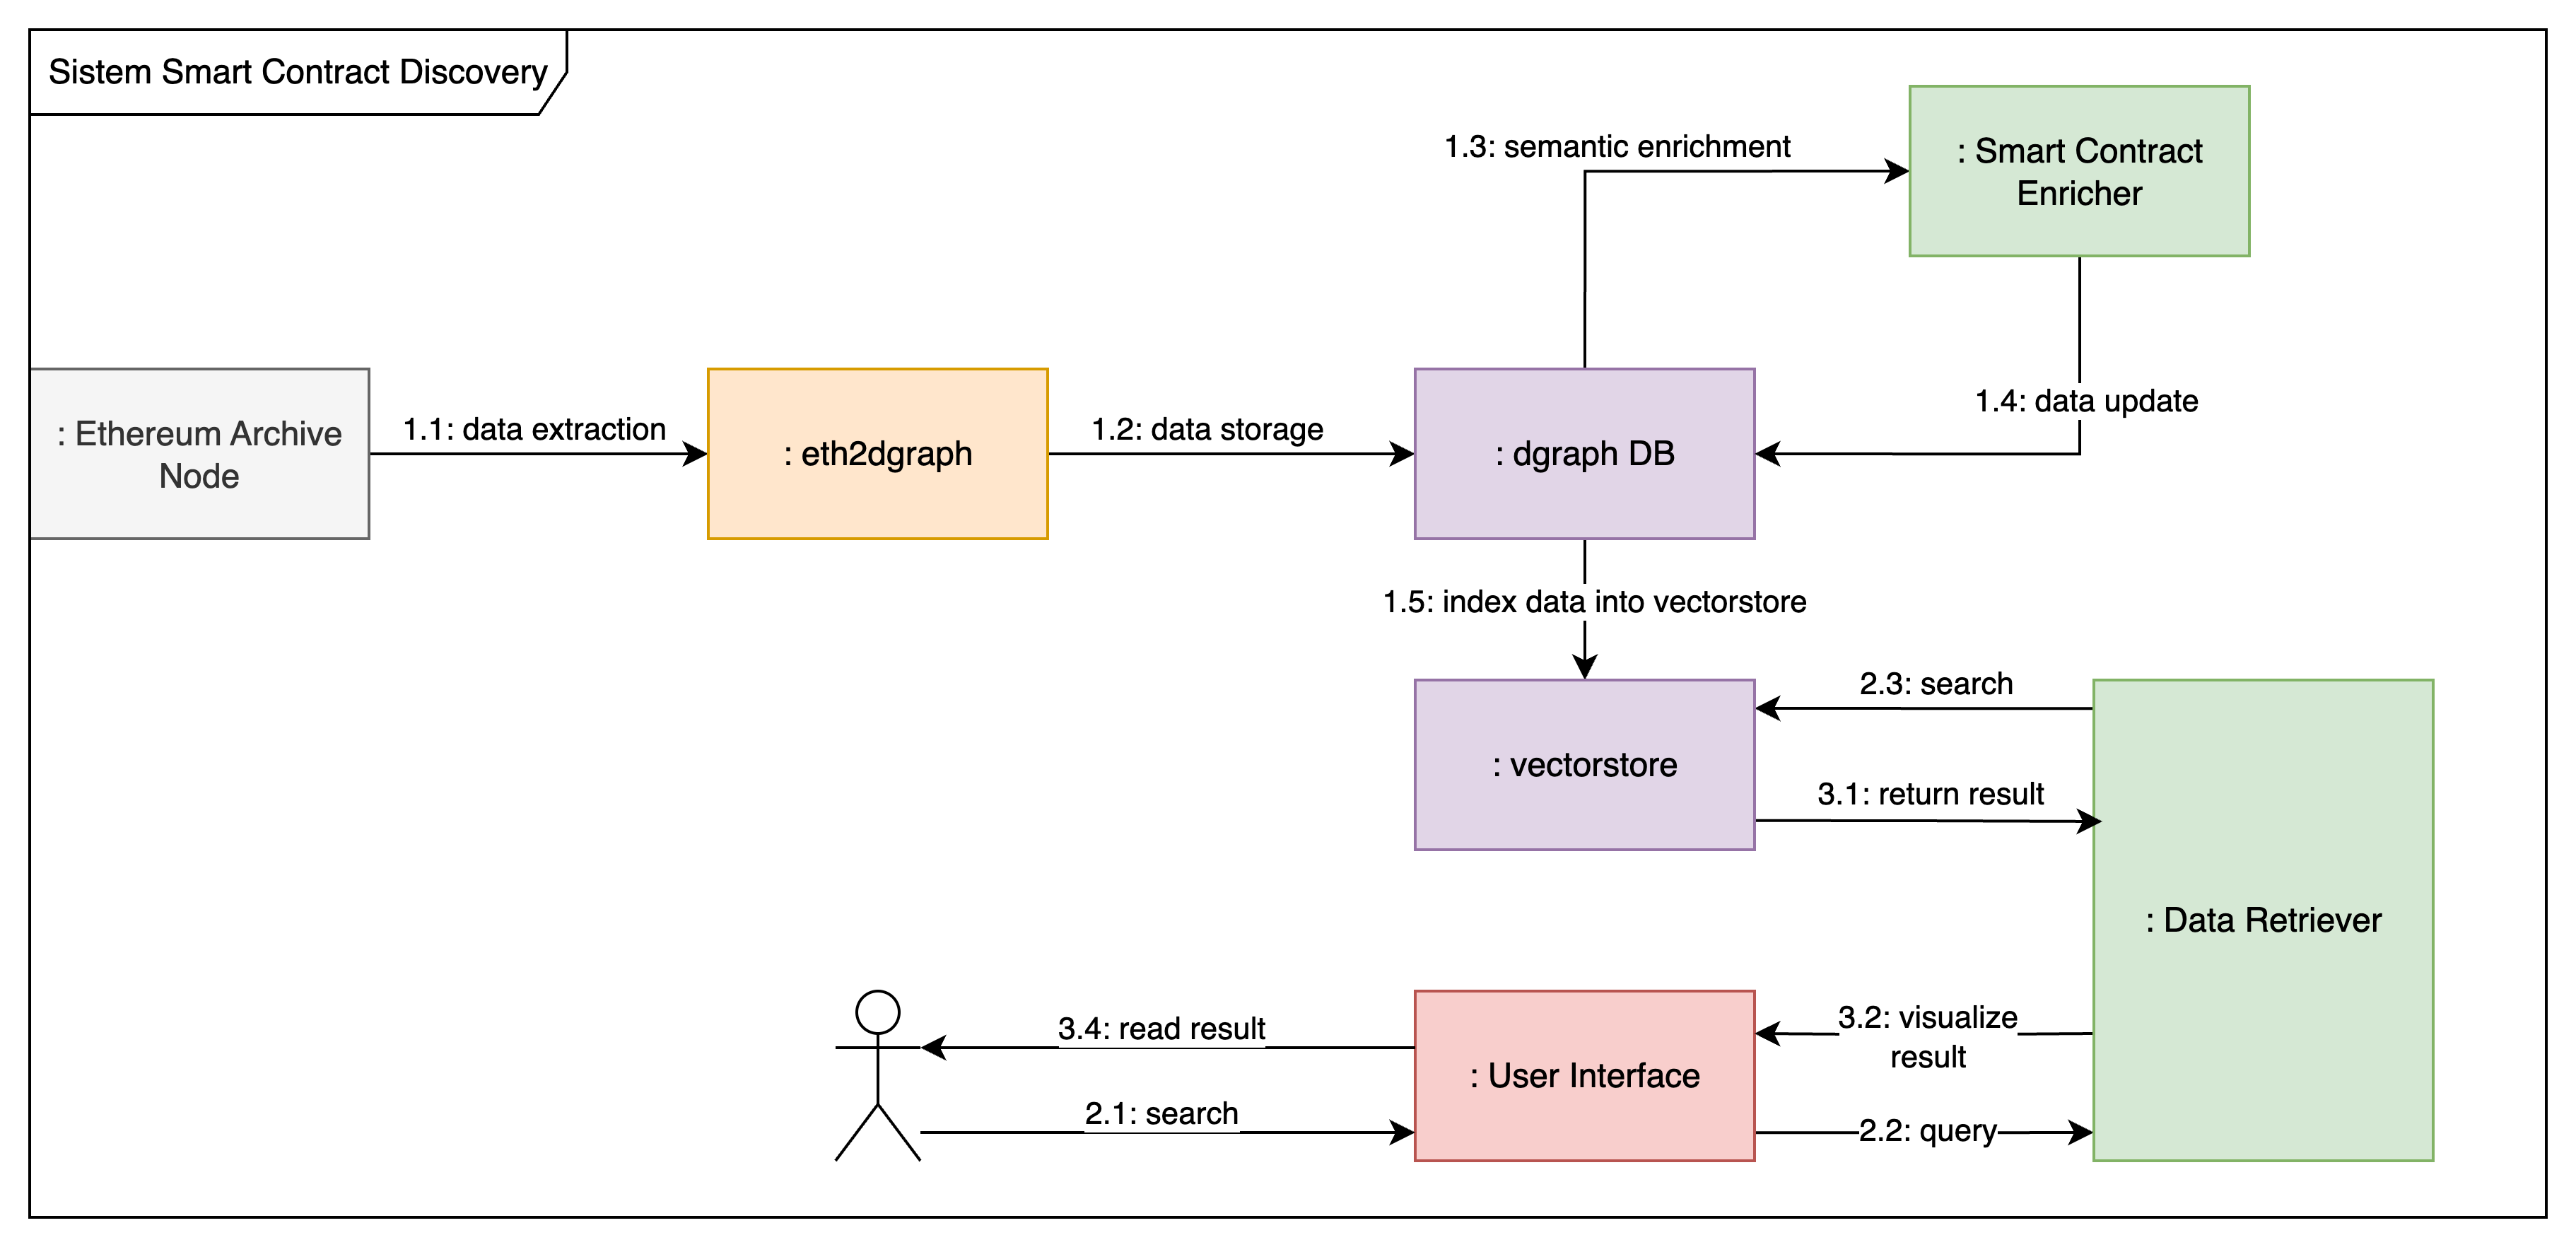
\includegraphics[width=1\textwidth]{resources/chapter-3/komponen-utama-new.png}
	\caption{Gambaran Umum Interaksi Komponen Utama Sistem}
	\label{image:komponen-sistem}
\end{figure}

\begin{figure}[ht]
	\centering
	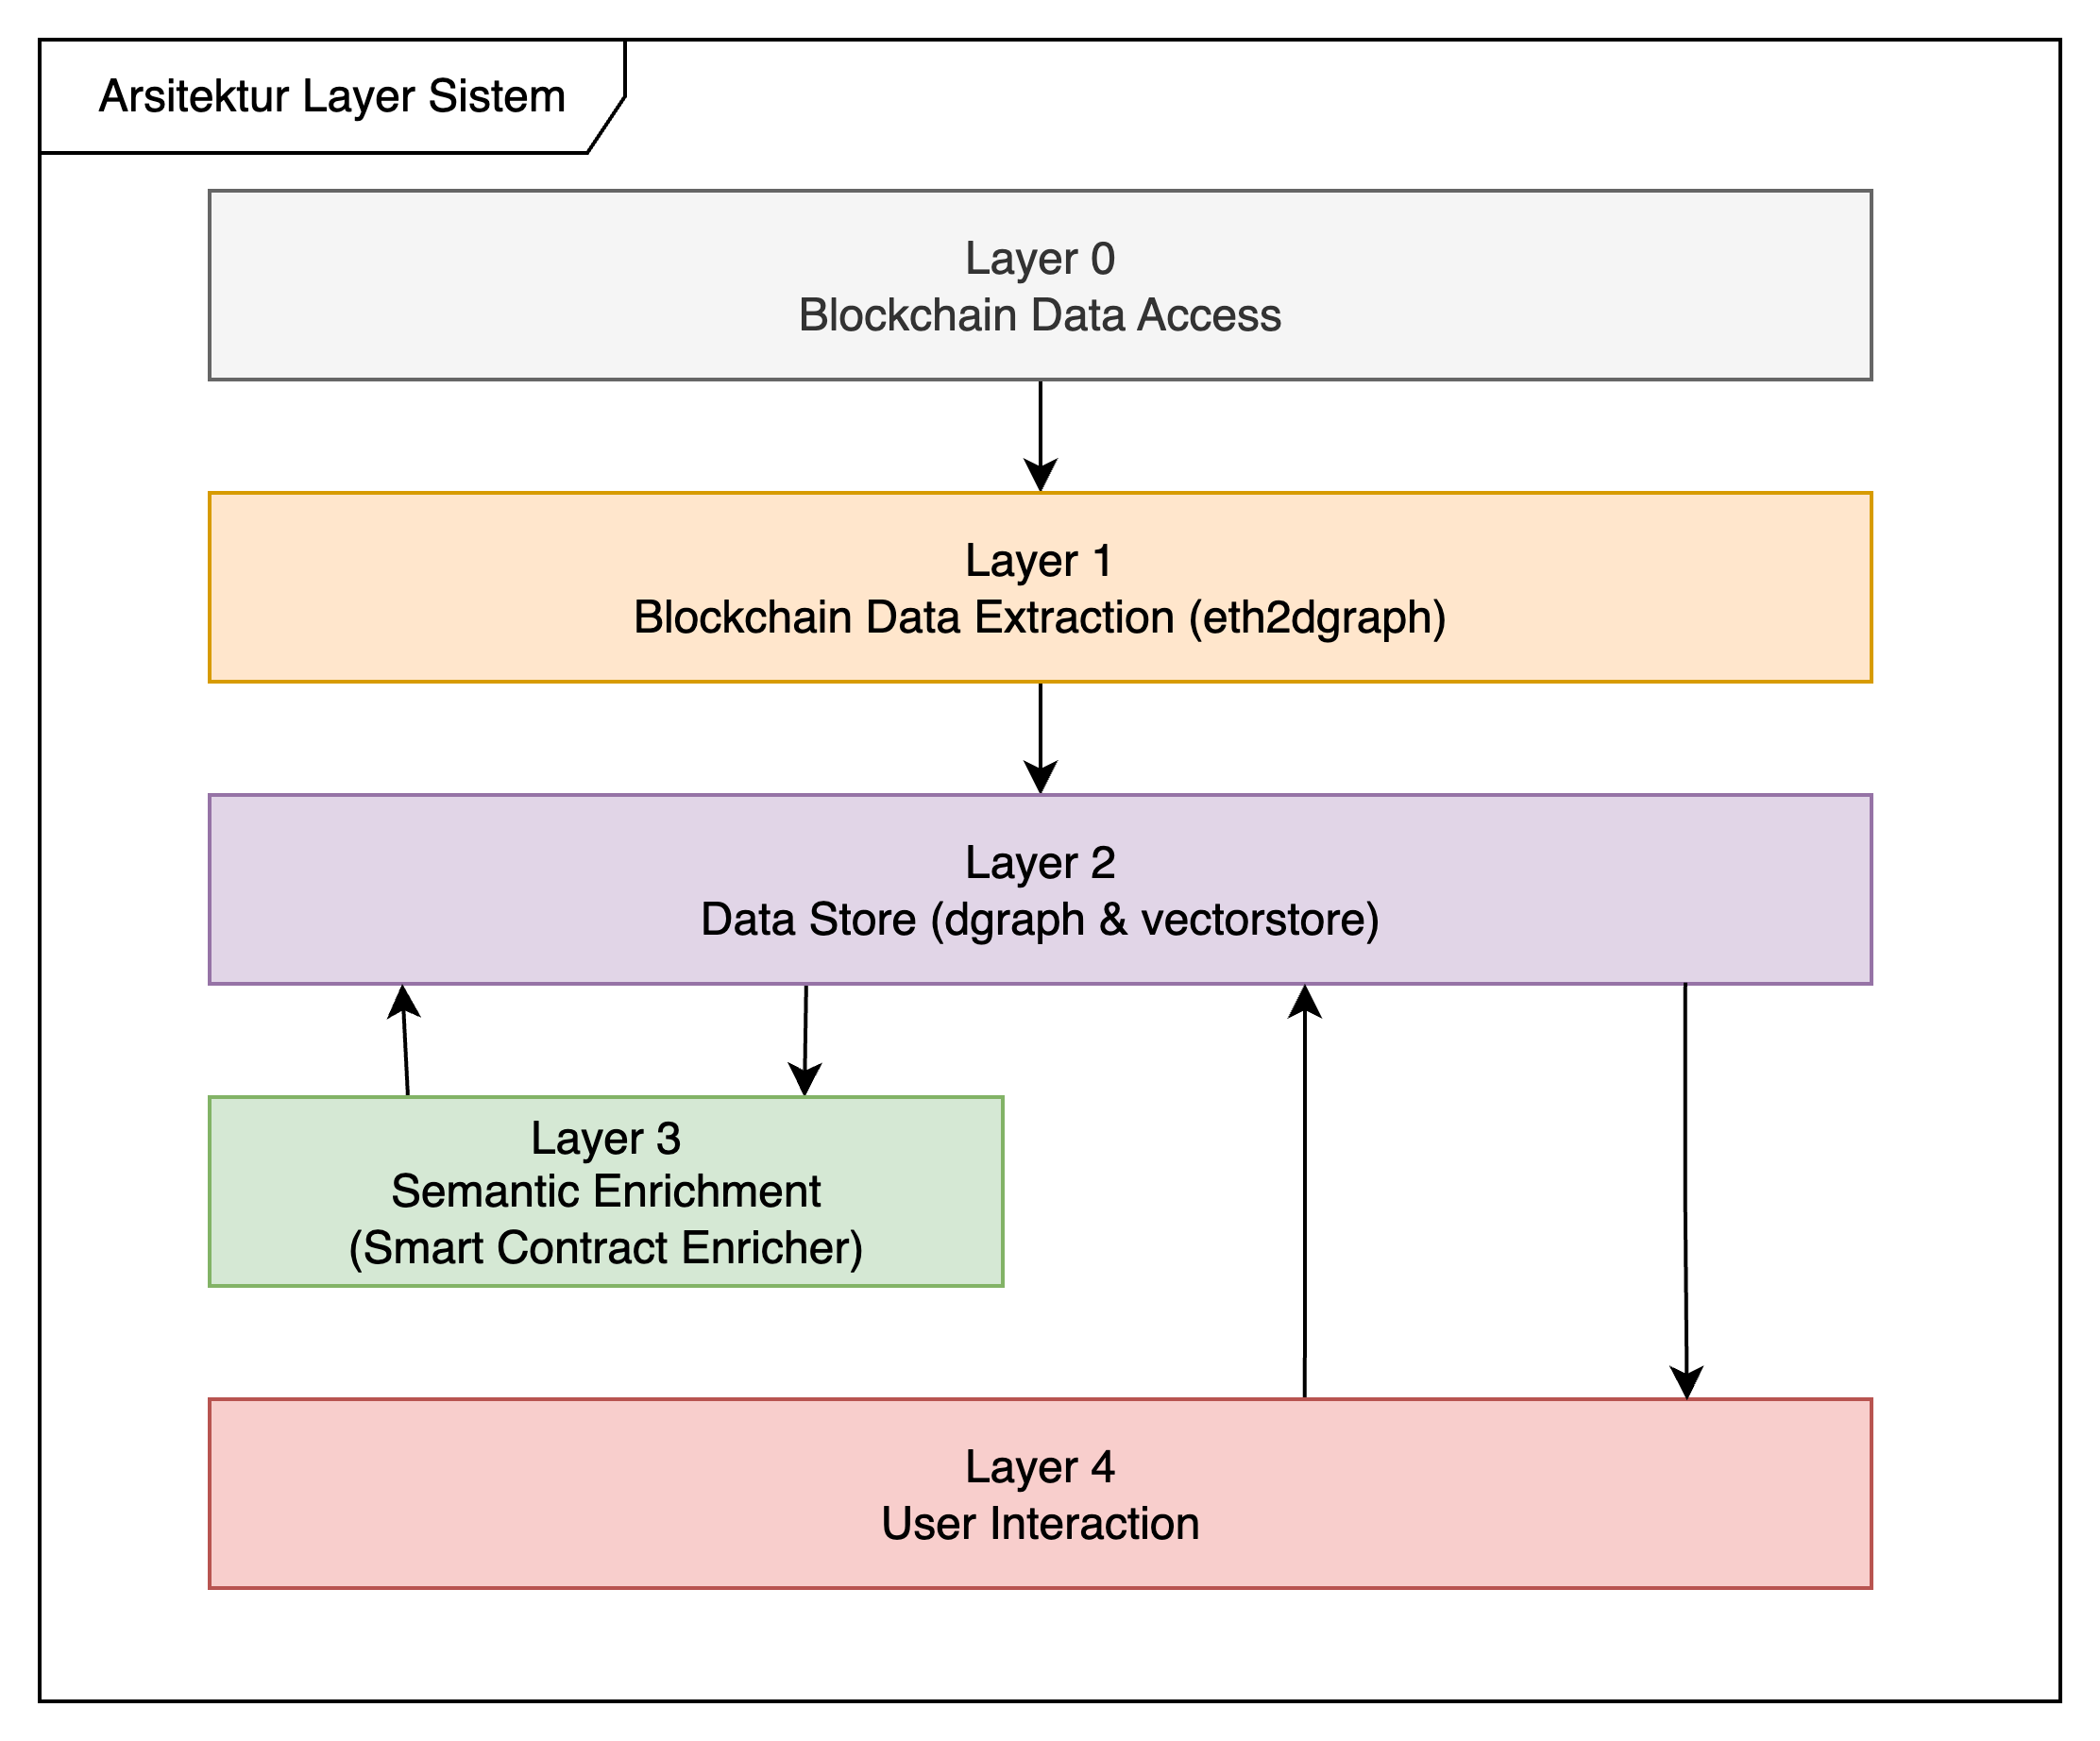
\includegraphics[width=0.7\textwidth]{resources/chapter-3/layer-arsitektur-new.png}
	\caption{Gambaran Arsitektur Layer Sistem}
	\label{image:layer-arsitektur}
\end{figure}

% Ethereum Archive Node → eth2dgraph (ekstraksi) → Dgraph (penyimpanan) → LLM (semantic enrichment) → Dgraph (update) → RAG (query).  

Gambar \ref{image:komponen-sistem} dan gambar \ref{image:layer-arsitektur} menunjukkan gambaran umum alur kerja sistem. Sistem ini akan melakukan ekstraksi data dari Ethereum Archive Node menggunakan \textit{eth2dgraph} dan menyimpannya dalam Dgraph. Setelah itu, sistem akan melakukan \textit{semantic enrichment} menggunakan LLM untuk memperkaya deskripsi dan metadata Smart Contract, lalu memperbarui data di Dgraph. Sebelum data dapat dilakukan query menggunakan RAG, akan dilakukan indexing data menjadi bentuk vectorstore. Terakhir, sistem akan menggunakan RAG untuk melakukan pencarian berdasarkan kebutuhan pengguna. 



\subsubsection{Karakteristik Pengguna}

Sistem ini hanya akan digunakan oleh satu jenis pengguna, yaitu User yang ingin mencari Smart Contract. Belum ada mekanisme yang membutuhkan campur tangan pengguna lain, seperti pengembang atau administrator. Pengguna dapat melakukan pencarian Smart Contract berdasarkan kebutuhan fungsionalitas yang diinginkan. Pengguna tidak perlu memiliki pengetahuan teknis yang mendalam tentang Smart Contract atau Blockchain untuk menggunakan sistem ini. Antarmuka pengguna dirancang agar mudah digunakan dan intuitif, sehingga pengguna dapat dengan mudah menemukan Smart Contract yang sesuai dengan kebutuhan mereka, dan menggunakannya, baik digunakan secara langsung, atau menjadi komponen di dalam aplikasi yang lebih besar.

\subsubsection{Kebutuhan Fungsional}

Sistem ini memiliki beberapa kebutuhan fungsional yang harus dipenuhi agar dapat berfungsi dengan baik. Kebutuhan fungsional ini mencakup semua fitur dan fungsi yang harus ada dalam sistem untuk memenuhi tujuan utama sistem. Berikut adalah daftar kebutuhan fungsional yang diidentifikasi:

% tabel
% \begin{table}[h]
% 	\caption{Kebutuhan Fungsional Sistem}
% 	\vspace{0.25cm}
% 	\begin{center}
% 		\begin{tabular}{|c|l|}
% 			\hline
% 			\textbf{ID} & \textbf{Penjelasan} \\ \hline
% 			F01 & User dapat melakukan input kebutuhan dalam bentuk \textit{Natural Language} \\ \hline
% 			F02 & User dapat mencari Smart Contract  \\ \hline
% 			F03 & Pengembangan Prototipe \\ \hline
% 			F04 & Pengujian Prototipe \\ \hline
% 			F05 & Evaluasi dan Perbaikan \\ \hline
% 		\end{tabular}
% 	\end{center}
% \end{table}

\subsubsection{Kebutuhan Non-Fungsional}

\subsubsection{Model Use Case}

Kebutuhan fungsional dan karakteristik pengguna yang dirumuskan dapat dimodelkan menjadi use case. Seperti pada gambar \ref{image:usecase}, Use case kemudian dapat dipetakan menjadi sebuah Use Case Diagram yang menghubungkan relasi antara aktor dengan use case yang berkolerasi. Diagram ini menggambarkan interaksi antara pengguna dan sistem, serta fungsi-fungsi yang tersedia dalam sistem. Diagram use case ini akan membantu dalam memahami bagaimana pengguna akan berinteraksi dengan sistem dan fitur-fitur apa saja yang harus ada dalam sistem. Use case dapat dilihat secara detail pada lampiran XX.

\begin{figure}[ht]
	\centering
	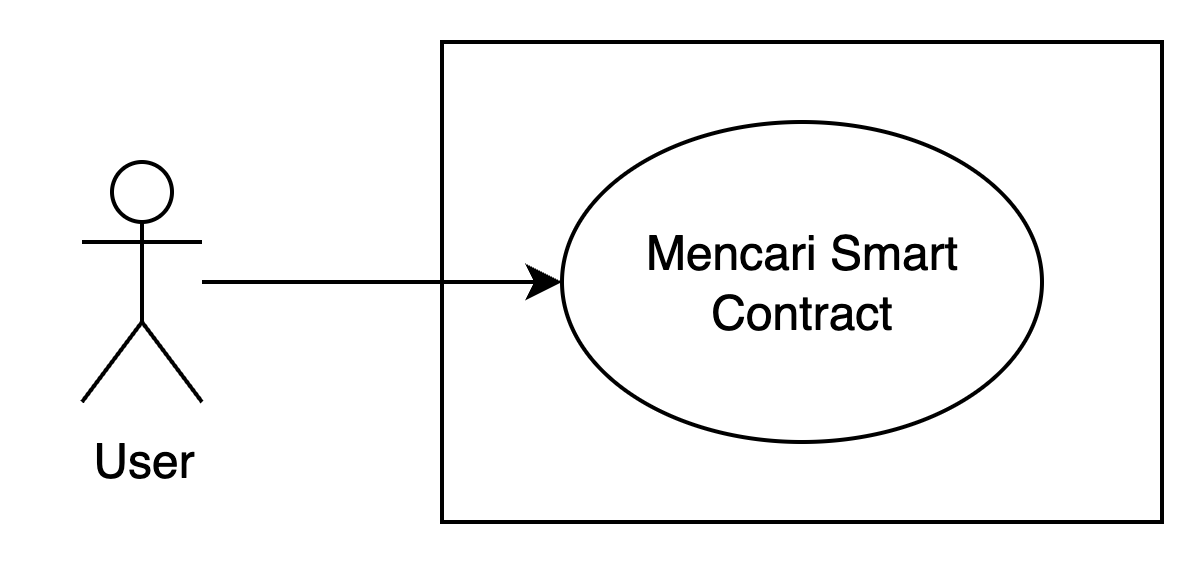
\includegraphics[width=0.7\textwidth]{resources/chapter-3/use-case.png}
	\caption{Use Case Diagram}
	\label{image:usecase}
\end{figure}

\subsubsection{Risiko dan Mitigasi}


\break

\section{Rancangan}

Bagian ini akan menjelaskan terkait rancangan sistem yang akan dibangun. Rancangan akan mencakup rancangan struktural, rancangan behavioral, dan rancangan detail dari setiap komponen. Sistem Smart Contract Discovery ini, seperti pada gambar \ref{image:komponen-sistem}, terdiri dari 5 komponen utama yang saling berinteraksi satu sama lain. Komponen-komponen tersebut adalah:

\begin{enumerate}
	\item Ethereum Archive Node: \textit{Node} Ethereum yang digunakan untuk melakukan ekstraksi data dari blockchain Ethereum. Berada pada eksternal sistem.
	\item eth2dgraph: Komponen yang digunakan untuk melakukan ekstraksi data dari Ethereum Archive Node dan menyimpannya ke dalam DgraphDB. Berada pada eksternal sistem.
	\item DgraphDB: Komponen yang digunakan untuk menyimpan data Smart Contracts yang sudah diekstraksi dari Ethereum Archive Node sekaligus data vector embeddings dari Smart Contracts yang telah diperkaya. Diperlukan modul data access untuk mengakses data dari DgraphDB dan mentransformasi data ke dalam bentuk vector embeddings.
	\item Smart Contract Enricher: Komponen yang digunakan untuk melakukan klasifikasi dan \textit{enrichment} data Smart Contracts.
	      % \item Vector Database: Komponen yang digunakan untuk menyimpan data Smart Contracts yang sudah diklasifikasikan dan di-\textit{enrich} oleh Smart Contract Enricher. Diperlukan modul data access untuk mengakses data dari Vector Database dan mentransformasi data ke dalam bentuk vector embedding.
	      % \item Query Enricher dan Data Retriever: Komponen yang digunakan untuk melakukan \textit{enrichment} terhadap query yang diberikan oleh pengguna dan melakukan data retrieval dari Vector Database.
	\item User Interface: Komponen yang digunakan untuk berinteraksi dengan pengguna. Terdapat dua jenis antarmuka yang akan dibangun, yaitu antarmuka berbasis \textit{API} dan antarmuka berbasis \textit{GUI}.
\end{enumerate}

\subsection{Rancangan Struktural}
\label{subsec:rancangan-struktural}

Arsitektur sistem yang akan dibangun akan digambarkan dengan Package Diagram. Sistem akan dibagi menjadi 3 kelompok komponen utama, yaitu eth2dgraph sebagai komponen luar sistem yang akan mengakses Ethereum Archive Node, komponen sistem utama yang terdiri dari DgraphDB dengan modul data access yang menyertakan modul transformasi data menjadi \textit{embeddings} dan pencarian data menggunakan \textit{embeddings}, Smart Contract Enricher, serta API yang akan mengekspos fungsi-fungsi yang ada pada sistem, dan komponen GUI. Ilustrasi dari rancangan struktural sistem dapat dilihat pada gambar \ref{image:rancangan-struktural}.

\begin{figure}[ht]
	\centering
	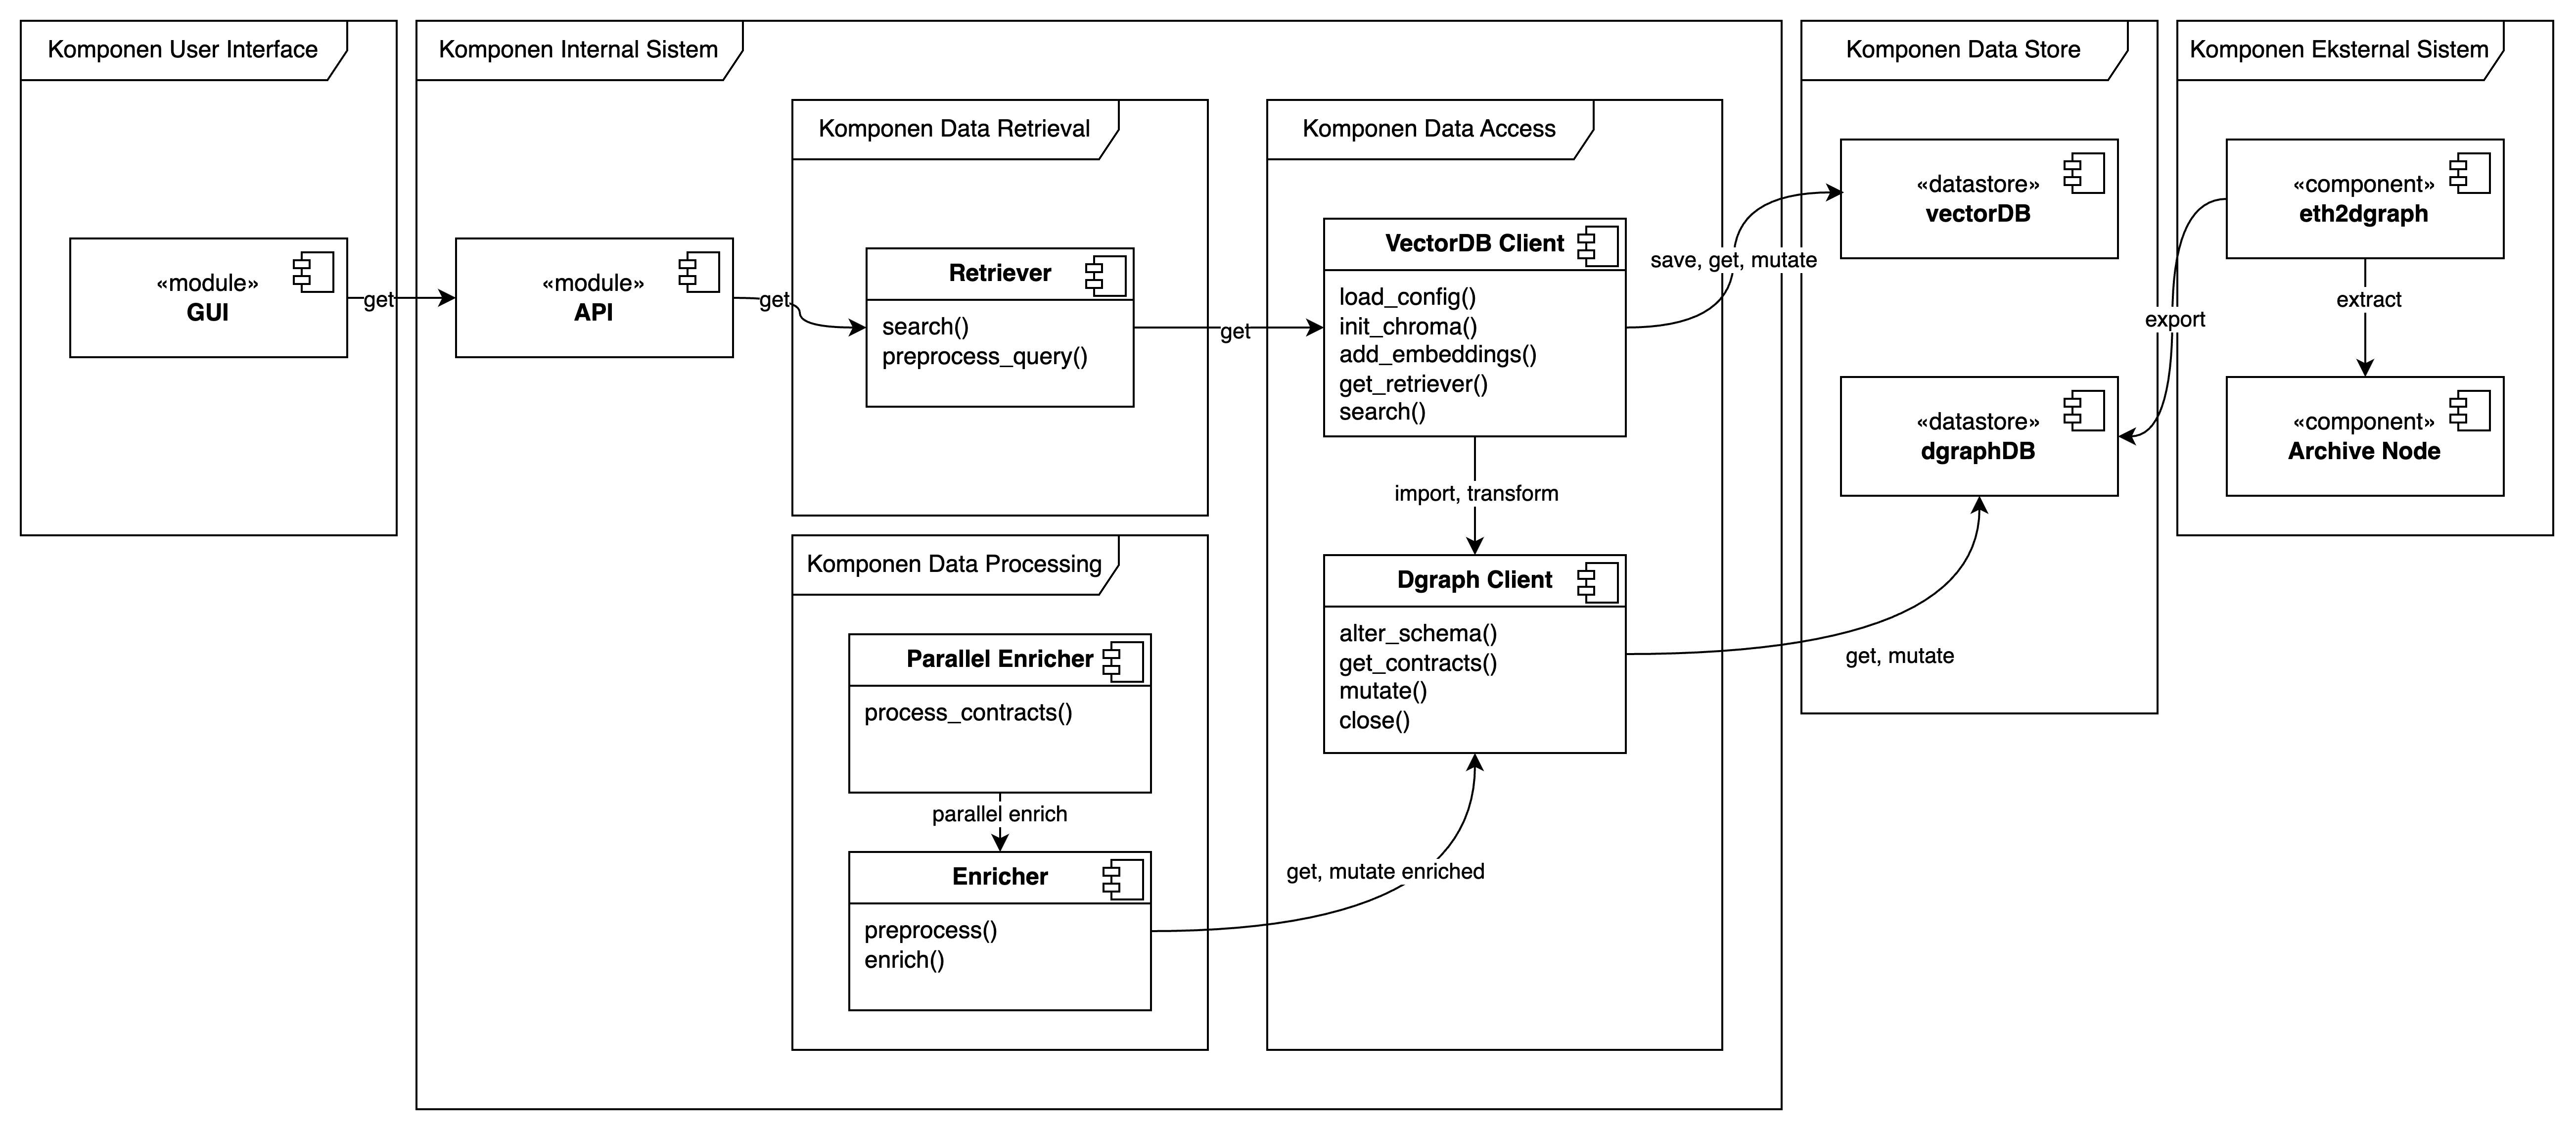
\includegraphics[width=1\textwidth]{resources/chapter-3/struktural.png}
	\caption{Rancangan struktural sistem}
	\label{image:rancangan-struktural}
\end{figure}

\subsection{Rancangan Behavioral}

Berdasarkan Use Case yang telah dirumuskan, terdapat 2 skenario utama yang akan dilakukan oleh pengguna, yaitu pencarian Smart Contracts dan pengambilan data address dari Smart Contracts. Selain itu, terdapat juga skenario tambahan yang terjadi di dalam sistem tanpa campur tangan pengguna, yaitu ekstraksi data Smart Contracts dari Blockchain, transformasi data Smart Contracts ke dalam Dgraph Database, Semantic Enrichment pada data Smart Contracts, transformasi data Smart Contracts menjadi vector embeddings, dan penyimpanan vector embeddings ke dalam Vector Database.

\subsubsection{Alur Mencari Smart Contract}

Pengguna akan melakukan pencarian dengan menggunakan API atau GUI. Pengguna akan memasukkan bahasa alami yang mendeskripsikan kebutuhan Smart Contract yang dicari. Data masukan yang diterima akan diteruskan ke API lalu ke komponen Retriever, yang akan melakukan query enrichment dan mengirimkan query ke dalam Vector Database dalam bentuk embedding. Hasil pencarian yang didapatkan akan dikembalikan ke API dan ditampilkan kepada pengguna dalam bentuk tabel yang berisi informasi Smart Contract yang relevan dengan query yang dimasukkan oleh pengguna. Ilustrasi alur pencarian Smart Contract dapat dilihat pada Gambar \ref{image:alur-pencarian-smart-contract}.

\begin{figure}[ht]
	\centering
	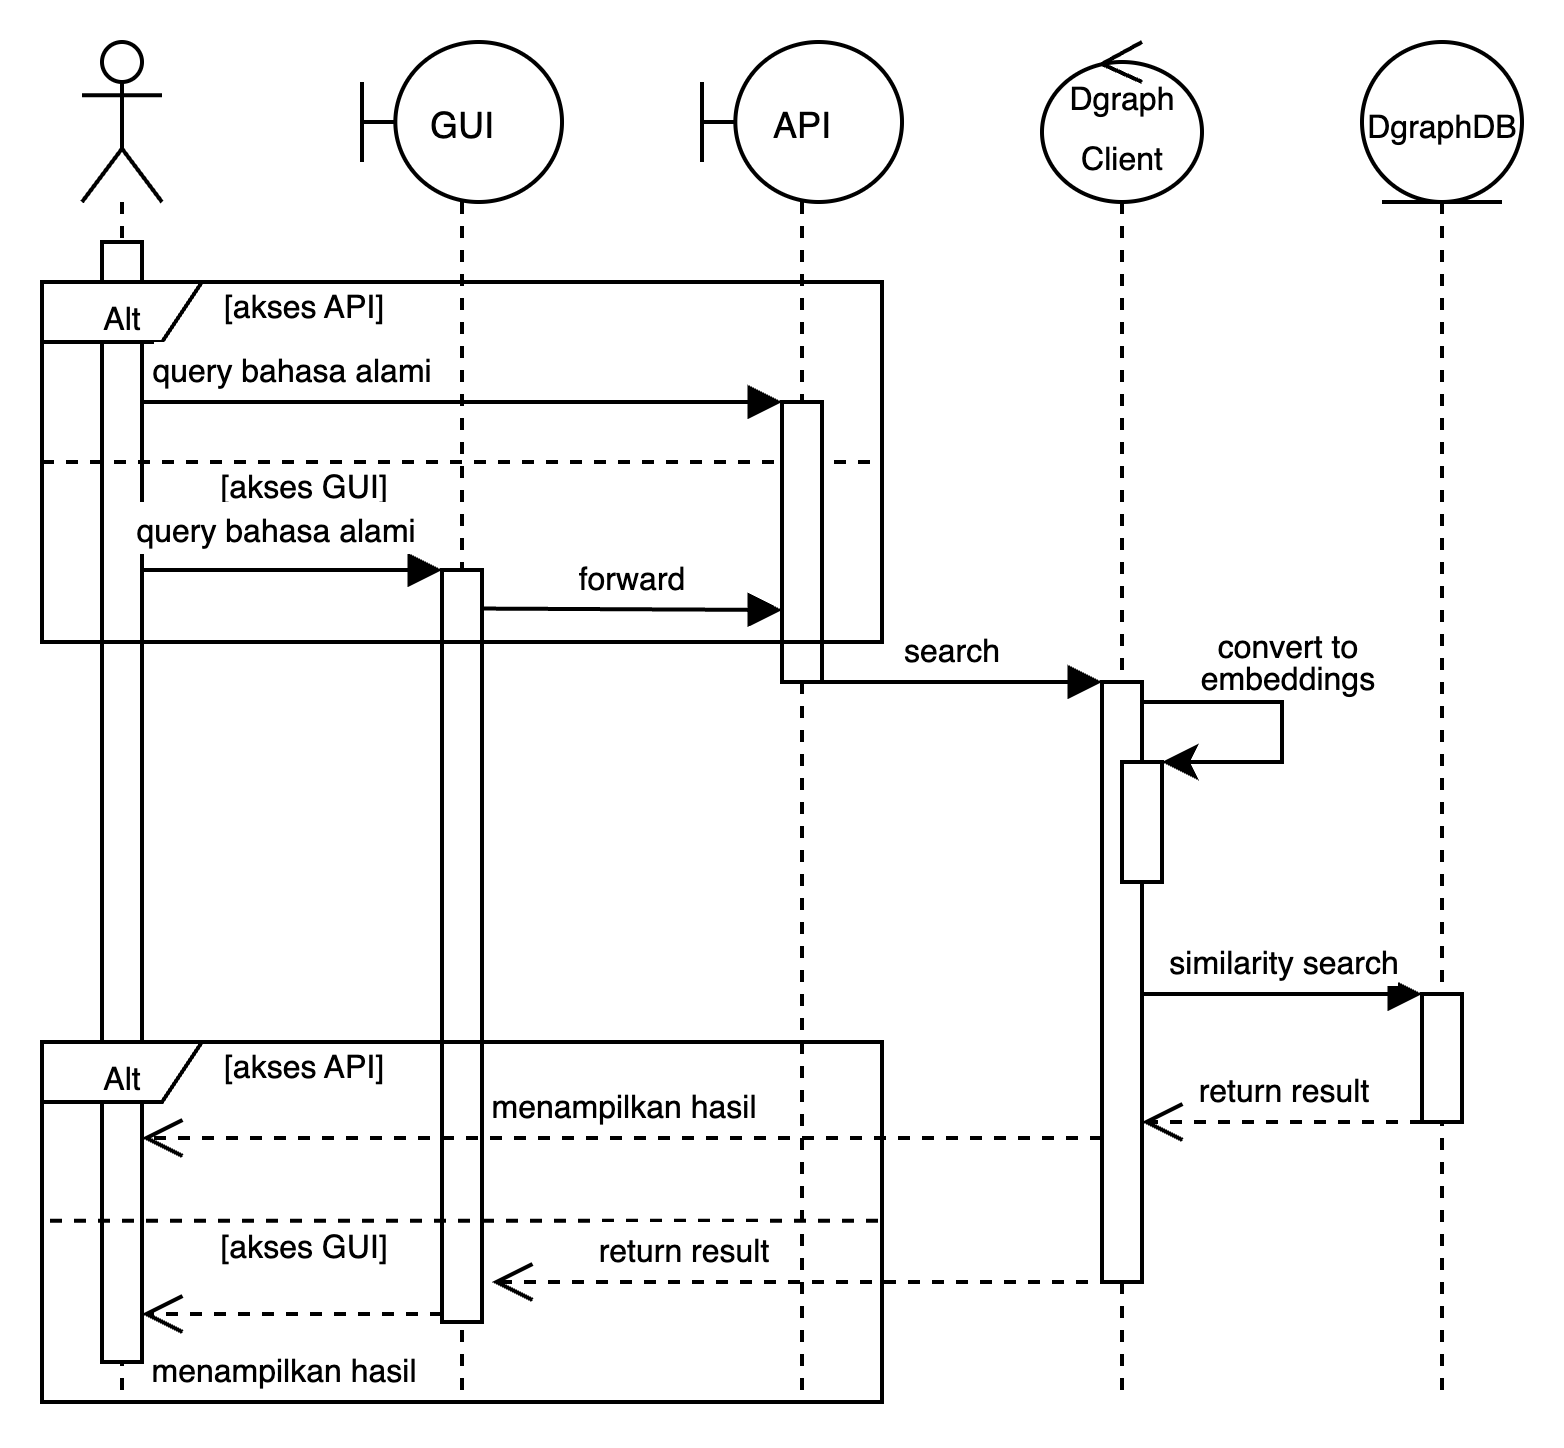
\includegraphics[width=0.7\textwidth]{resources/chapter-3/sequence-1.png}
	\caption{Alur Pencarian Smart Contract}
	\label{image:alur-pencarian-smart-contract}
\end{figure}

\subsubsection{Alur Mendapatkan Address Smart Contract}

Pengguna akan melakukan pencarian dengan menggunakan API atau GUI. Pengguna akan memasukkan dgraph ID yang didapatkan dari hasil pencarian Smart Contract. Data ID yang diterima akan diteruskan ke API lalu ke dgraph Client, yang akan melakukan query ke dalam Dgraph Database. Hasil pencarian yang didapatkan akan dikembalikan ke API dan ditampilkan kepada pengguna dalam bentuk tabel yang berisi informasi Smart Contract dengan dgraph ID yang dimasukkan oleh pengguna. Ilustrasi alur mendapatkan address Smart Contract dapat dilihat pada Gambar \ref{image:alur-mendapatkan-address-smart-contract}.

\begin{figure}[ht]
	\centering
	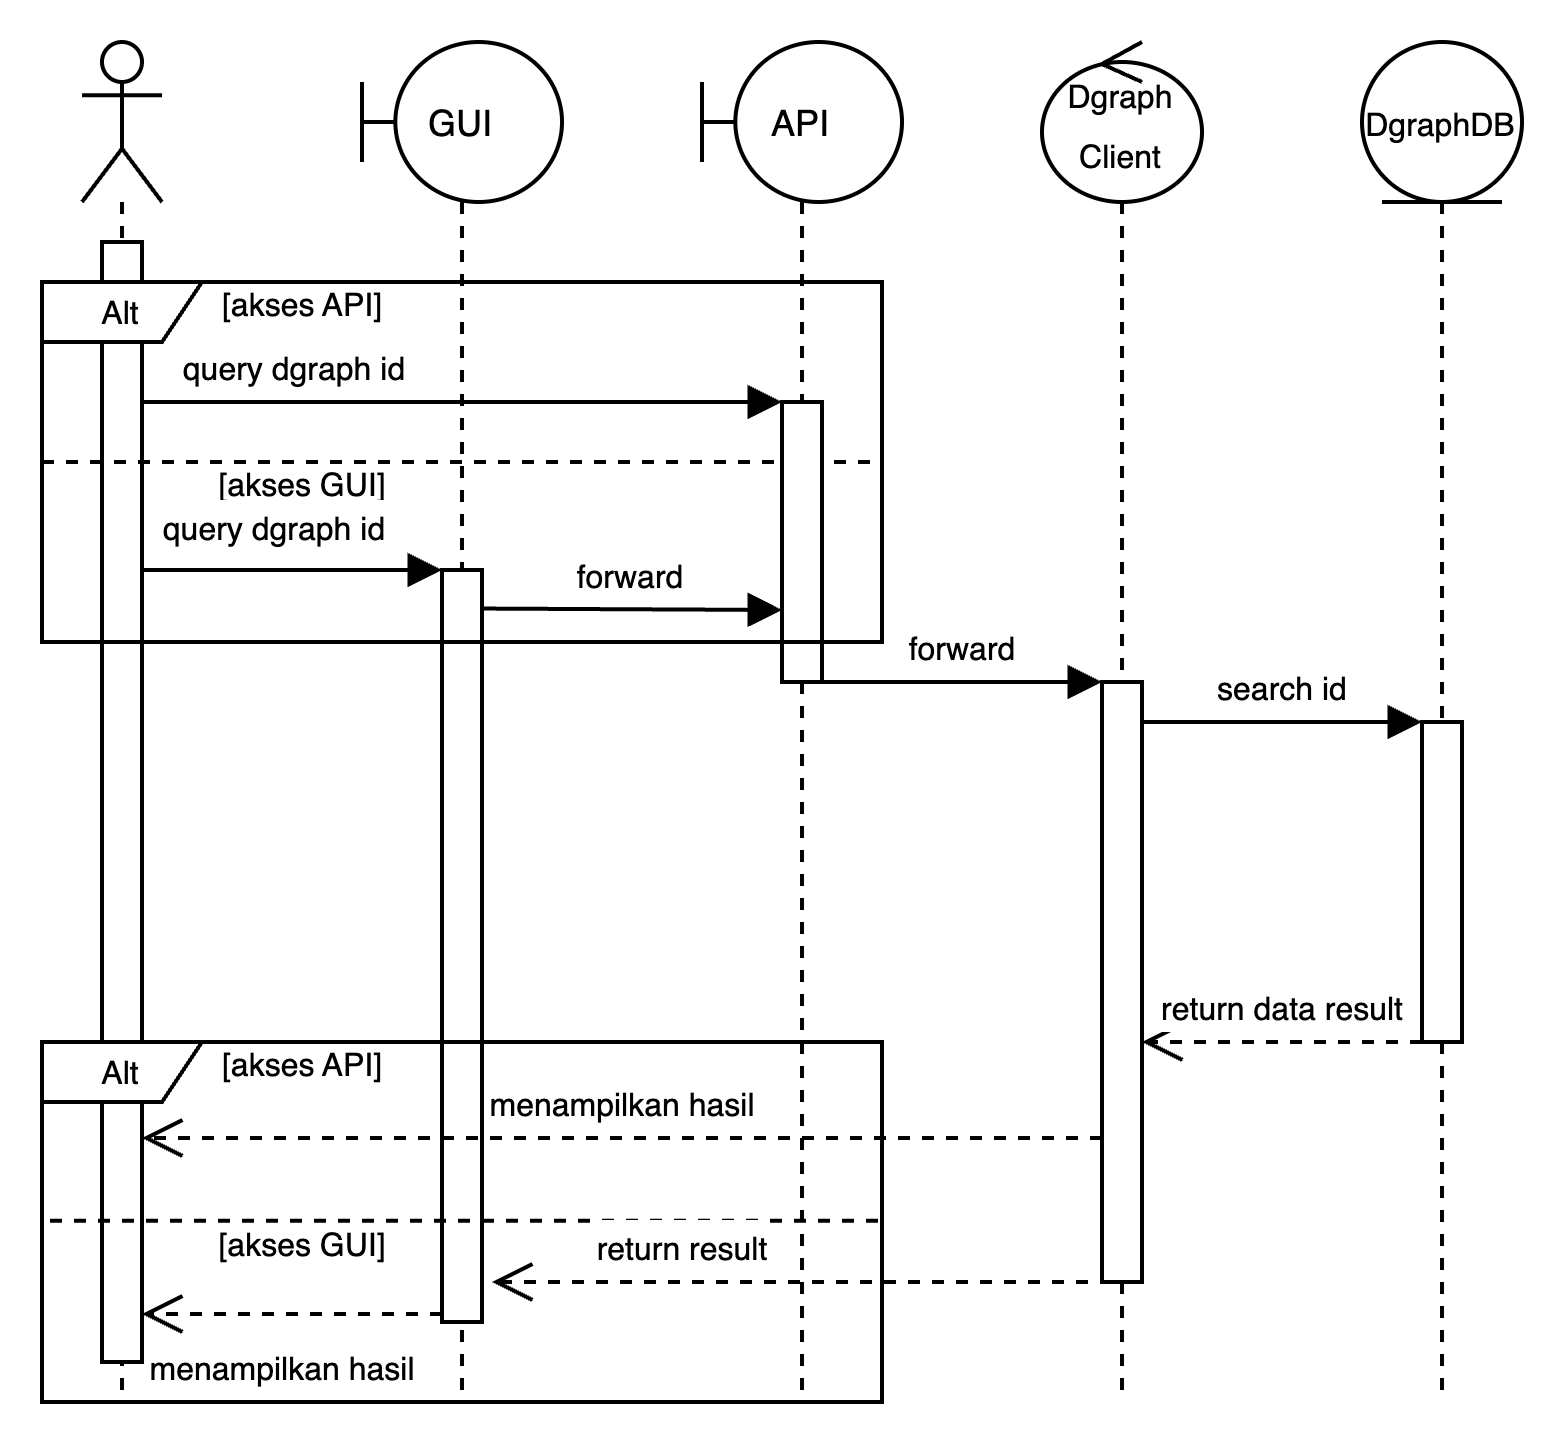
\includegraphics[width=0.7\textwidth]{resources/chapter-3/sequence-2.png}
	\caption{Alur Mendapatkan Address Smart Contract}
	\label{image:alur-mendapatkan-address-smart-contract}
\end{figure}

% \subsubsection{Alur Ekstraksi Data}

% \subsubsection{Alur Transformasi Data Menjadi Dgraph}

% \subsubsection{Alur Semantic Enrichment}

% \subsubsection{Alur Transformasi Data Menjadi Vector Embeddings}

% \subsubsection{Alur Penyimpanan Vector Embeddings}

\subsection{Rancangan Detail Komponen}

\subsubsection{Rancangan Detail Komponen GUI}

Komponen GUI akan digunakan sebagai salah satu antarmuka pengguna untuk berinteraksi dengan sistem. Komponen ini akan menyediakan tampilan sederhana yang memungkinkan pengguna untuk memasukkan query dalam bahasa alami, melihat hasil pencarian Smart Contracts, dan mendapatkan informasi lebih lanjut tentang Smart Contracts yang relevan. Komponen GUI akan berkomunikasi dengan API untuk mengirimkan query dan menerima hasil pencarian.

Terdapat 3 tampilan utama pada komponen GUI, yaitu:
\begin{itemize}
	\item Tampilan Pencarian Smart Contract: Pengguna dapat memasukkan query dalam bahasa alami untuk mencari Smart Contracts yang relevan dan mendapatkan daftar hasil pencarian Smart Contracts dengan informasi umum terkait Smart Contracts yang didapatkan.
	\item Tampilan Detail Smart Contract: Menampilkan informasi lebih lanjut tentang Smart Contract yang dipilih, termasuk address, deskripsi, dan metadata lainnya.
	\item Tampilan Import Smart Contract: Menampilkan cara melakukan import Smart Contract yang khusus untuk Smart Contract yang dipilih, sehingga pengguna dapat dengan mudah mengimport Smart Contract tersebut.
\end{itemize}

\subsubsection{Rancangan Detail Komponen API}

Komponen API akan menjadi antarmuka utama bagi pengguna untuk berinteraksi dengan fungsinoalitas sistem. Komponen ini akan menerima permintaan dari pengguna, memproses permintaan tersebut, dan mengembalikan respons yang sesuai. Komponen API akan berkomunikasi dengan komponen Dgraph Client untuk melakukan pencarian Smart Contracts dan mendapatkan informasi lengkap dari Smart Contracts.

Komponen API akan menyediakan satu endpoint utama untuk menerima query dalam bahasa alami dari pengguna. Endpoint ini akan menerima permintaan pencarian, meneruskan query ke komponen Dgraph Client, dan mengembalikan hasil pencarian kepada pengguna.

% \subsubsection{Rancangan Detail Komponen Retriever}

% Komponen Retriever akan bertanggung jawab untuk melakukan pencarian Smart Contracts berdasarkan query yang diberikan oleh pengguna. Komponen ini akan menerima query dari komponen API, melakukan query expansion untuk meningkatkan relevansi hasil pencarian, dan kemudian melakukan pencarian menggunakan interface yang disediakan oleh VectorDB Client. Hasil pencarian akan dikembalikan ke komponen API untuk ditampilkan kepada pengguna.

\subsubsection{Rancangan Detail Komponen Enricher}
% Bahas terkait schema disini

Komponen Enricher akan bertanggung jawab untuk memperkaya data Smart Contracts yang akan disimpan dalam VectorDB. \textit{Enrichment} ini dilakukan untuk membantu meningkatkan kualitas dan relevansi data yang disimpan, sehingga memudahkan proses pencarian dan pengambilan informasi.

Komponen Enricher terbagi menjadi 2 subkomponen, yaitu:
\begin{enumerate}
	\item \textbf{Semantic Enricher}: Subkomponen ini akan melakukan proses pengayaan data Smart Contracts secara paralel. Proses ini akan memperkaya data dengan informasi tambahan yang relevan, seperti metadata, deskripsi, dan informasi lainnya yang dapat membantu dalam pencarian dan pengambilan informasi.
	\item \textbf{Data Schema}:
	      Subkomponen skema akan diterapkan kepada data Smart Contracts yang akan disimpan dalam DgraphDB. Skema ini akan memastikan bahwa data yang disimpan memiliki struktur yang konsisten dan dapat mendeskripsikan semantik Smart Contracts. Skema ini akan mencakup atribut-atribut penting dari Smart Contracts, seperti address, deskripsi, fungsionalitas, metadata, dan informasi lainnya yang relevan.
\end{enumerate}

Proses yang dilakukan oleh komponen Enricher adalah sebagai berikut:
\begin{enumerate}
	\item Komponen Enricher akan mengambil data Smart Contracts yang disimpan pada DgraphDB.
	\item Data \textit{source code} dari Smart Contracts akan diambil dan dilakukan preprocessing sehingga dapat diproses dengan lebih efisien.
	\item Data Smart Contracts akan diproses oleh subkomponen Semantic Enricher untuk melakukan data enrichment. Proses ini akan menghasilkan data yang lebih kaya dan relevan.
	\item Setelah proses pengayaan selesai, data yang telah diperkaya akan disimpan kembali ke dalam DgraphDB. Proses penyimpanan ini akan menggunakan komponen Dgraph Client untuk memastikan bahwa data yang disimpan sesuai dengan skema yang telah ditentukan.
\end{enumerate}

\subsubsection{Rancangan Detail Komponen Parallel Enricher}

Komponen Parallel Enricher merupakan sebuah komponen \textit{wrapper} untuk komponen Semantic Enricher. Komponen ini akan membagi \textit{task} untuk enrichment dan menjalankan proses enrichment secara paralel. Hal ini dilakukan untuk meningkatkan efisiensi dan kecepatan proses pengayaan data Smart Contracts.

% \subsubsection{Rancangan Detail Komponen VectorDB Client}

% Komponen VectorDB Client akan bertanggung jawab untuk berkomunikasi dengan VectorDB yang digunakan untuk menyimpan dan mengambil data embeddings dari Smart Contracts yang sudah dilakukan enrichment. Komponen ini akan menyediakan fungsi untuk mengakses fungsionalitas pencarian semantik dari VectorDB. Terdapat sebuah skrip untuk melakukan \textit{pull} data dari DgraphDB, mengonversi menjadi embeddings, dan menyimpannya ke dalam VectorDB. Skrip ini akan dijalankan secara berkala untuk memastikan bahwa data yang disimpan di VectorDB selalu diperbarui dengan data terbaru dari DgraphDB.

\subsubsection{Rancangan Detail Komponen Dgraph Client}

Komponen Dgraph Client akan bertanggung jawab untuk berkomunikasi dengan DgraphDB yang digunakan untuk menyimpan data Smart Contracts dan embeddings dari Smart Contracts. Komponen ini akan menyediakan fungsi untuk melakukan query, penyimpanan, mutasi skema, penambahan embeddings, pencarian berdasarkan embeddings dan pengambilan data dari DgraphDB. Komponen ini akan menjadi antarmuka utama bagi komponen lain untuk berinteraksi dengan DgraphDB. Pencarian berdasarkan embeddings ini akan dilakukan menggunakan cosine similarity, dengan abstraksi fungsi yang diberikan oleh Dgraph dengan query \texttt{similar\textunderscore to}. Cosine similarity dapat menentukan kedekatan semantik dari sebuah teks dengan teks lainnya berdasarkan arah dari vector embeddings-nya.

% package diagram
% sesuai domain, ada class diagramnya



% \chapter{Implementasi dan Pengujian}
\chapter{Rencana Pelaksanaan}

Bab ini akan menjelaskan proses implementasi dari rancangan solusi yang telah dikaji pada Bab III. Setelah pembahasan terkait implementasi, akan dilanjutkan dengan pemaparan hasil uji terkait implementasi yang telah dibuat.


% Bab Rencana Pelaksanaan digunakan untuk mendeskripsikan rencana pelaksanaan berupa jadwal dan risiko-risiko yang mungkin dihadapi dan rencana mitigasinya. Tujuan bab ini  adalah:
% 1.	Mahasiswa memiliki rencana yang jelas mengenai pelaksanaan TA
% 2.	Mahasiswa mengenali risiko-risiko yang mungkin dihadapi dan sudah menyiapkan diri untuk mengantisipasi risiko tersebut.

% \section{Lingkungan}
% \blindtext

% \section{Implementasi}
% \blindtext

% \section{Pengujian}
% \blindtext

\section{Jadwal}
\label{sec:jadwal}

% Cantumkan jadwal pengerjaan tugas akhir lengkap dengan uraiannya.

\section{Risiko}
\label{sec:risiko}

% misal kegiatan apa yang akan jadi tantangan, misal ada kepengurusan, jadi lebih baik dituliskan agar diperhatikan
% misal kurang banyak artikel yang dituliskan

% Cantumkan 5 risiko tertinggi yang mungkin dihadapi dalam pengerjaan tugas akhir. Risiko yang dicantumkan dapat merupakan risiko dari sisi teknis, risiko dari sisi operasional, risiko dari metode yang dipilih, dan sebagainya. Cantumkan pula rencana mitigasi dari risiko-risiko tersebut.

% \chapter{Penutup}

Bab Kesimpulan dan Saran akan menjadi bagian akhir dan penutup dari penelitian tugas akhir ini. Bagian ini akan merangkum ketercapaian dari penelitian terhadap ukuran keberhasilan yang telah ditetapkan dan memberikan saran-saran yang dapat digunakan untuk mengembangkan penelitian ini lebih lanjut.

\section{Kesimpulan}

Berdasarkan keseluruhan proses penelitian, pengembangan sistem, perbaikan, pengujian, dan analisis hasil yang dilakukan pada penelitian tugas akhir ini, dapat ditarik beberapa kesimpulan sebagai berikut:

\begin{enumerate}
    \item Penelitian tugas akhir ini telah berhasil mengembangkan sebuah sistem pencarian Smart Contracts berbasis semantik dengan pendekatan LLM \textit{enrichment}.
    \item Sistem ini telah dievaluasi dengan menggunakan perbandingan dengan sistem pencarian berbasis teks pada Source Code dan deskripsi semantik yang dihasilkan. Hasil pengujian menunjukkan bahwa pencarian pada deskripsi semantik memberikan peningkatan relevansi hasil pencarian dan pencarian berbasis semantik memberikan hasil yang terbaik dibandingkan dengan metode pencarian lainnya. Sistem pencarian berbasis semantik ini diimplementasikan dengan analisis Source Code oleh LLM dan \textit{enrichment} data yang difasilitasi dengan prompt dan embeddings yang telah dikembangkan. Poin ini menjawab rumusan masalah pertama terkait metode \textit{enrichment} yang dapat memberikan pengertian semantik pada data.
    \item Sistem ini memiliki mengambil data dari blockchain Ethereum mainnet, menyimpan data tersebut dalam format yang telah ditentukan, melakukan \textit{enrichment} dengan LLM, menyimpan data yang sudah enriched dan melakukan pencarian berbasis semantik menggunakan cosine similarity pada embeddings yang dihasilkan atau teks deskripsi yang dihasilkan. Deskripsi semantik yang dihasilkan dari sistem ini dapat disesuaikan dengan mengubah format yang digunakan untuk menyimpan data dan prompt yang digunakan untuk melakukan \textit{enrichment}. Sehingga, sistem ini dapat dengan mudah di-\textit{extend} untuk meningkatkan relevansi hasilnya. Selain itu, sistem ini telah diuji dan dibandingkan dengan pencarian berbasis teks dan mendapatkan hasil presisi yang lebih baik. Poin ini menjawab rumusan masalah kedua terkait metode \textit{data retrieval} berbasis semantik yang efektif. 
    \item Fungsionalitas sistem ini untuk menerima input berupa kebutuhan pengguna dalam bahasa alami dan menghasilkan daftar Smart Contract yang relevan telah berhasil diimplementasikan. Sistem ini dapat menerima input berupa bahasa alami, kata kunci, atau teks deskripsi yang relevan dengan Smart Contracts yang dicari. Sistem ini juga dapat memberikan daftar hasil pencarian yang relevan dengan kebutuhan pengguna. Poin ini menjawab rumusan masalah ketiga terkait fungsionalitas sistem Smart Contract Discovery.
    \item Format semantik yang digunakan tersedia pada lampiran dari laporan ini. Format ini dapat mengakomodasi berbagai jenis fungsionalitas dan juga domain yang berbeda. Poin ini adalah pemenuhan tujuan pertama dari tugas akhir ini.
    \item Teknik \textit{semantic enrichment} yang digunakan adalah teknik dan prompt yang telah dikembangkan. Teknik yang digunakan adalah dengan menggunakan LLM untuk menganalisis Source Code Smart Contract dan melakukan \textit{enrichment} pada data berdasarkan prompt yang disediakan. Prompt ini tersedia pada lampiran dari laporan ini. Poin ini adalah pemenuhan tujuan kedua dari tugas akhir ini.
    \item \textit{Data retrieval} yang digunakan adalah pencarian embeddings yang disediakan oleh Dgraph. Pencarian ini dilakukan dengan menggunakan cosine similarity pada embeddings yang dihasilkan dari proses \textit{enrichment}. Poin ini adalah pemenuhan tujuan ketiga dari tugas akhir ini.
    \item Mekanisme ektraksi data dan konversi menjadi format yang dapat digunakan oleh sistem telah berhasil diimplementasikan memanfaatkan eth2dgraph. Mekanisme ini dilakukan dengan menggunakan Archive Node untuk mendapatkan data dan Dgraph untuk menyimpan data dan melakukan query terhadap data yang disimpan. Poin ini adalah pemenuhan tujuan keempat dari tugas akhir ini.
    \item Sistem Smart Contract Discovery telah berhasil diimplementasikan dan dapat digunakan untuk mencari Smart Contracts yang relevan dengan kebutuhan pengguna. Sistem ini dapat diakses melalui API dan Web GUI yang telah disediakan. Poin ini adalah pemenuhan tujuan kelima dari tugas akhir ini.
\end{enumerate}
 
\section{Saran}
Meskipun sistem Smart Contract Discovery berbasis semantik ini telah berhasil dikembangkan, terdapat beberapa saran yang dapat diberikan untuk pengembangan penelitian ini lebih lanjut. Saran-saran ini berisi kekurangan sistem yang teridentifikasi serta peluang pengembangan yang dapat dilakukan untuk meningkatkan sistem ini.

\begin{enumerate}
    \item Format semantik yang digunakan masih dapat diperbaiki untuk meningkatkan relevansi hasil pencarian. Format yang digunakan saat ini masih cukup umum dan dapat diperluas untuk mengakomodasi fungsionalitas yang lebih spesifik. Pengembangan lebih lanjut dapat dilakukan untuk mengembangkan format semantik yang lebih spesifik secara domain dan relevan dengan kebutuhan pengguna.
    \item Prompt yang digunakan untuk melakukan \textit{enrichment} masih dapat diperbaiki untuk meningkatkan relevansi hasil pencarian. Prompt yang digunakan saat ini masih cukup umum dan dapat diperluas untuk mengakomodasi fungsionalitas yang lebih spesifik. Pengembangan lebih lanjut dapat dilakukan untuk mengembangkan prompt yang lebih spesifik secara domain dan relevan dengan kebutuhan pengguna.
    \item Model LLM yang digunakan saat ini adalah model OpenAI GPT4o mini, dimana sudah terdapat model-model yang lebih baik dan lebih murah yang dapat digunakan untuk melakukan \textit{enrichment}. Seiring model LLM yang lebih baik dan lebih murah berkembang, sistem ini dapat memanfaatkan perkembangan tersebut untuk meningkatkan relevansi hasil pencarian dan mengurangi biaya yang dikeluarkan untuk melakukan \textit{enrichment}.
    \item Pencarian berbasis semantik yang dilakukan masih terbatas pada kemampuan pengguna untuk memberikan query bahasa alami atau kata kunci yang sesuai dengan kebutuhan. Pada kenyataannya, tidak semua pengguna memiliki kemampuan tersebut. Terdapat peluang untuk mengembangkan sistem pencarian berbasis semantik yang dapat memahami kebutuhan pengguna dengan lebih baik, misalnya dengan menggunakan AI Agents untuk berinteraksi dengan pengguna dan memahami kebutuhan mereka secara lebih mendalam lalu melakukan pencarian berbasis semantik pada sistem menggunakan Model Context Protocol.
    \item Sistem ini dapat diperluas untuk memfasilitasi seluruh Smart Contracts, termasuk Smart Contracts yang tidak terverifikasi. Hal ini dilakukan dengan memanfaatkan penelitian analisis Bytecode yang tersedia. Namun, hal ini akan menambahkan risiko keamanan yang lebih tinggi karena sifat dari Smart Contracts yang tidak terverifikasi. Oleh karena itu, perlu dilakukan penelitian lebih lanjut untuk mengembangkan sistem yang dapat memfasilitasi Smart Contracts yang tidak terverifikasi dengan aman.
    \item Sistem retrieval dapat ditingkatkan dengan menggunakan teknik yang lebih canggih seperti \textit{knowledge graph} untuk meningkatkan relevansi semantik dari hasil pencarian. Hal ini dapat dilakukan dengan mengembangkan sistem yang dapat mengekstraksi entitas dan relasi dari Smart Contracts, sehingga dapat membangun \textit{knowledge graph} yang dapat digunakan untuk meningkatkan relevansi hasil pencarian.
    \item Sistem retrieval dapat ditingkatkan dengan mengekstraksi nilai-nilai yang ada dari data, membangun sebuah ontologi, yang lalu akan digunakan oleh sebuah model AI yang menerima input dari pengguna lalu mengubah input tersebut menjadi sebuah query yang spesifik menggunakan ontologi yang dimiliki. Hal ini dapat meningkatkan relevansi dan menghasilkan hasil yang lebih spesifik sesuai dengan kebutuhan pengguna.
    \item Sistem retrieval dapat ditingkatkan dengan menggabungkan beberapa teknik seperti teknik \textit{reranking} hasil dengan menggabungkan pendekatan berbasis teks dan berbasis semantik. Hal ini dapat meningkatkan relevansi hasil pencarian dengan menggabungkan kekuatan dari kedua pendekatan tersebut.
    \item Sistem retrieval dapat ditingkatkan dengan menambahkan mekanisme chunking untuk konversi embeddings pada Source Code Smart Contracts. Hal ini dapat dimanfaatkan untuk melakukan pencarian semantik pada embeddings Source Code.
\end{enumerate}


%---------------------------------------------------------------%

% Daftar pustaka
\printbibliography

% Setting judul lampiran
\titlespacing*{\chapter}{0pt}{0pt}{0pt}
\titlespacing*{\section}{0pt}{0pt}{*1}

% Setting judul anak lampiran
\titleformat*{\section}{\bfseries}

\appendix

\chapter{Skema Data}
\label{appendix:skema-data}

\begin{lstlisting}[language=bash]
    <ContractDeployment.block>: uid @reverse .
    <ContractDeployment.contract>: uid @reverse .
    <ContractDeployment.creation_bytecode>: string .
    <ContractDeployment.creator>: uid @reverse .
    <ContractDeployment.deployed_bytecode>: string .
    <ContractDeployment.experimental>: bool .
    <ContractDeployment.failed_deploy>: bool .
    <ContractDeployment.solc_version>: string .
    <ContractDeployment.storage_address>: string .
    <ContractDeployment.storage_protocol>: string .
    <ContractDeployment.tx_hash>: string @index(hash) .
    <ContractDeployment.name>: string @index(trigram) .
    <ContractDeployment.verified_source>: bool @index(bool) .
    <ContractDeployment.verified_source_code>: string @index(term) .
    <ContractDeployment.description>: string @index(fulltext) .
    <ContractDeployment.functionality_classification>: string @index(fulltext) .
    <ContractDeployment.application_domain>: string @index(fulltext) .
    <ContractDeployment.security_risks_description>: string @index(fulltext) .
    <ContractDeployment.embeddings>: float32vector @index(hnsw(metric:"euclidean")) .
\end{lstlisting}


\chapter{Perintah eth2dgraph}
\label{appendix:eth2dgraph-commands}

\begin{enumerate}
	\item \texttt{extract}
	      \begin{enumerate}
		      \item \texttt{-e, --endpoint <ENDPOINT>}: RPC endpoint dari Archive Node
		      \item \texttt{-o, --output <OUTPUT\textunderscore PATH>}: output path dari hasil ekstraksi
		      \item \texttt{-f, --from-block <FROM\textunderscore BLOCK>}: nomor blok awal dari ekstraksi
		      \item \texttt{-t, --to-block <TO\textunderscore BLOCK>}: nomor blok akhir dari ekstraksi
		      \item \texttt{-n, --num-tasks <NUM\textunderscore TASKS>}: jumlah Tokio \textit{tasks} yang akan dijalankan secara paralel
		      \item \texttt{--include-tx}: flag untuk menyertakan transaksi dalam ekstraksi
		      \item \texttt{--include-transfers}: flag untuk menyertakan transfer dalam ekstraksi
		      \item \texttt{--include-logs}: flag untuk menyertakan log dalam ekstraksi
		      \item \texttt{-s, --scs-path <SCS\textunderscore PATH>}: path Smart Contract Sanctuary untuk disambungkan dengan data yang diekstrak
		      \item \texttt{--size-output <SIZE\textunderscore OUTPUT>}: ukuran maksimal di dalam RAM untuk output files sebelum di-\textit{flush} dan dikompresi ke \textit{disk}, dalam KB
		      \item \texttt{--compression-level <COMPRESSION\textunderscore LEVEL>}: tingkat kompresi \\hasil ekstraksi dari 0 (tanpa kompresi) hingga 9 (kompresi maksimal)
		      \item \texttt{--decompiler-timeout <DECOMPILER\textunderscore TIMEOUT>}: waktu maksimal untuk dekompilasi Smart Contract, dalam milliseconds
		      \item \texttt{--skip-decompilation}: flag untuk melewati proses ekstraksi ABI dengan heimdall
	      \end{enumerate}
	\item \texttt{stream}
	      \begin{enumerate}
		      \item \texttt{-e, --endpoint <ENDPOINT>}: endpoint Ethereum Archive Node \\yang akan dihubungkan dengan skema websocket
		      \item \texttt{-d, --dgraph <DGRAPH>}: endpoint GRPC Dgraph
		      \item \texttt{--include-tx}: flag untuk menyertakan transaksi dalam \textit{streaming}
		      \item \texttt{--include-tokens}: flag untuk menyertakan transfer token dalam \textit{streaming}
		      \item \texttt{--include-logs}: flag untuk menyertakan log dalam \textit{streaming}
		      \item \texttt{--decompiler-timeout <DECOMPILER\textunderscore TIMEOUT>}: waktu maksimal untuk dekompilasi Smart Contract, dalam milliseconds
		      \item \texttt{--no-sync}: flag untuk melewati sinkronisasi dari blok terakhir yang diindeks di Dgraph, hanya mengambil blok live
		      \item \texttt{-n, --num-jobs <NUM\textunderscore JOBS>}: jumlah Tokio \textit{tasks} yang akan dijalankan secara paralel
	      \end{enumerate}
	\item \texttt{analyse}
	      \begin{enumerate}
		      \item \texttt{similarities}: analisis kesamaan antar Smart Contract
		            \begin{enumerate}
			            \item \texttt{-e, --endpoint <ENDPOINT>}: endpoint GRPC Dgraph
			            \item \texttt{-o, --output-file <OUTPUT\textunderscore FILE>}: file output dari hasil analisis
			            \item \texttt{-a, --address <ADDRESS>}: alamat Smart Contract untuk menghitung kesamaan
			            \item \texttt{--interface-sim}: flag untuk menghitung kesamaan interface
			            \item \texttt{--interface-threshold <INTERFACE\textunderscore THRESHOLD>}: ambang \\batas minimum kesamaan interface (0.0-1.0) di atas mana kesamaan akan disimpan
			            \item \texttt{--cosine-sim}: flag untuk menghitung kesamaan cosine
			            \item \texttt{--cosine-threshold <COSINE\textunderscore THRESHOLD>}: ambang batas minimum kesamaan cosine (0.0-1.0) di atas mana kesamaan akan disimpan
			            \item \texttt{--ngram-length <NGRAM\textunderscore LENGTH>}: panjang N-gram yang digunakan untuk kesamaan cosine
		            \end{enumerate}
		      \item \texttt{lifetimes}: analisis lifetime Smart Contract
		            \begin{enumerate}
			            \item \texttt{-e, --endpoint <ENDPOINT>}: endpoint GRPC Dgraph
			            \item \texttt{-o, --output-path <OUTPUT\textunderscore PATH>}: path output dari hasil analisis
			            \item \texttt{-c, --cache-file <CACHE\textunderscore FILE>}: file cache yang akan digunakan
		            \end{enumerate}
	      \end{enumerate}
\end{enumerate}

\chapter{Docker Compose File}
\label{appendix:docker-compose-dgraph}

\begin{lstlisting}[language=bash]
    version: "3.2"

    services:
    zero:
        image: dgraph/dgraph:latest
        volumes:
        - ./dgraph:/utils:ro
        - ./dgraph-data:/dgraph
        ports:
        - 5081:5080
        - 6081:6080
        restart: on-failure
        command: 'dgraph zero --my=zero:5080'
    alpha:
        image: dgraph/dgraph:latest
        working_dir: /dgraph/out/0
        volumes:
        - ./dgraph-data:/dgraph
        ports:
        - 8081:8080
        - 9081:9080
        restart: on-failure
        command: 'dgraph alpha --my=alpha:7080 --zero=zero:5080 --security whitelist=0.0.0.0/0 --badger="compression=snappy; numgoroutines=64;" '
    ratel:
        image: dgraph/ratel:latest
        ports:
        - 8001:8000

    volumes:
    grafana-data:
\end{lstlisting}
\chapter{Perintah Dgraph}
\label{appendix:dgraph-commands}

\begin{enumerate}
	\item \texttt{dgraph alpha}: Perintah ini digunakan untuk menjalankan Dgraph Alpha, yang merupakan komponen utama dari DgraphDB yang bertanggung jawab untuk menyimpan dan mengelola data. Perintah ini akan menghubungkan Dgraph Alpha dengan Dgraph Zero dan menyediakan antarmuka HTTP untuk berinteraksi dengan data.
	\item \texttt{dgraph zero}: Perintah ini digunakan untuk menjalankan Dgraph Zero, yang merupakan komponen yang bertanggung jawab untuk Dgraph Cluster Management. Dgraph Zero akan mengelola metadata dari DgraphDB, termasuk informasi tentang shard dan replikasi data.
	\item \texttt{dgraph bulk}: Perintah ini digunakan untuk melakukan impor data ke dalam DgraphDB. Perintah ini akan mengambil data dari file yang telah diekstrak dan memprosesnya untuk dimasukkan ke dalam database. Berikut merupakan parameter dari perintah \texttt{dgraph bulk} yang dapat digunakan:
	      \begin{enumerate}
		      \item \texttt{-f, --files <FILES>}: lokasi file \texttt{*.rdf(.gz)} atau \texttt{*.json(.gz)} yang akan di-\textit{load}
		      \item \texttt{-s, --schema <SCHEMA>}: lokasi file skema
		      \item \texttt{-g, --graphql-schema <GRAPHQL\textunderscore SCHEMA>}: lokasi file skema GraphQL
		      \item \texttt{--out <OUT>}: lokasi untuk menyimpan direktori data dgraph final (default \texttt{./out})
		      \item \texttt{--map-shards <MAP\textunderscore SHARDS>}: jumlah \textit{map output shards}. Harus lebih besar atau sama dengan jumlah \textit{reduce shards}. Peningkatan memungkinkan \textit{reduce shards} berukuran lebih merata, dengan mengorbankan peningkatan penggunaan memori (default 1)
		      \item \texttt{--reduce-shards <REDUCE\textunderscore SHARDS>}: jumlah \textit{reduce shards}. Ini menentukan jumlah instans dgraph dalam kluster final. Peningkatan ini berpotensi mengurangi waktu eksekusi tahap \textit{reduce} dengan menggunakan lebih banyak paralelisme, tetapi meningkatkan penggunaan memori
		      \item \texttt{-z, --zero <ZERO>}: alamat gRPC untuk Dgraph zero
		      \item \texttt{--mapoutput-mb <MAPOUTPUT\textunderscore MB>}: perkiraan ukuran setiap output file \textit{map}. Peningkatan ini meningkatkan penggunaan memori (default 2048)
		      \item \texttt{-j, --num-go-routines <NUM\textunderscore GO\textunderscore ROUTINES>}: jumlah \textit{worker threads} yang digunakan. Semakin banyak \textit{threads} akan menyebabkan penggunaan RAM yang lebih tinggi (default 1)
		      \item \texttt{--tmp <TMP>}: direktori sementara yang digunakan untuk \textit{scratch space} pada disk. Memerlukan ruang kosong yang proporsional dengan ukuran file RDF dan jumlah pengindeksan yang digunakan (default \texttt{tmp})
		      \item \texttt{--replace-out}: mengganti direktori \textit{out} dan isinya jika sudah ada
		      \item \texttt{--cleanup-tmp}: membersihkan direktori \texttt{tmp} setelah \textit{loader} selesai. Mengatur ini menjadi \texttt{false} memungkinkan \textit{bulk loader} dapat dijalankan ulang sambil melewati fase \textit{map} (default \texttt{true})
		      \item \texttt{--badger <BADGER>}: opsi Badger (default \texttt{compression=snappy; numgoroutines=8;})
		            \begin{enumerate}
			            \item \texttt{compression}: menentukan algoritma kompresi dan tingkat kompresi untuk direktori \textit{postings}. \texttt{none} akan menonaktifkan kompresi, sedangkan \texttt{zstd:1} akan mengatur kompresi zstd pada tingkat 1
			            \item \texttt{numgoroutines}: jumlah \textit{goroutines} yang digunakan dalam \\\texttt{badger.Stream}
		            \end{enumerate}
	      \end{enumerate}
\end{enumerate}

\chapter{Dgraph Client}
\label{appendix:dgraph-client}

\begin{enumerate}
    \item \texttt{logger}: Objek logger yang mencatat informasi, peringatan, dan kesalahan pada operasi DgraphClient.
    \item \texttt{client\textunderscore stub}: Stub koneksi ke server Dgraph, berfungsi sebagai endpoint komunikasi.
    \item \texttt{client}: Klien tingkat tinggi yang membungkus stub untuk melakukan query dan mutasi.
    \item \texttt{embedding\textunderscore model}: Model HuggingFaceEmbeddings untuk mengubah teks menjadi vektor numerik guna pencarian berbasis vektor.
    \item \texttt{\textunderscore init\textunderscore }: Konstruktor yang menginisialisasi stub, klien, logger, dan model embedding.
    \item \texttt{generate\textunderscore contract\textunderscore id}: Menghasilkan ID kontrak deterministik berdasarkan atribut unik kontrak, termasuk hashing kode sumber terverifikasi.
    \item \texttt{dgraph\textunderscore txn}: Context manager untuk memulai transaksi Dgraph; melakukan commit pada transaksi tulis dan selalu melakukan discard di akhir.
    \item \texttt{alter\textunderscore schema}: Mengirim operasi untuk memperbarui skema Dgraph berdasarkan string skema yang diberikan.
    \item \texttt{get\textunderscore contracts}: Mengambil daftar kontrak dengan opsi paging (\texttt{batch\textunderscore \\size}, \texttt{offset}) dan filter \texttt{enriched} untuk memisahkan kontrak yang sudah berisi deskripsi.
    \item \texttt{get\textunderscore contract\textunderscore by\textunderscore id}: Mengambil data kontrak berdasarkan ID deterministik yang dihasilkan oleh \texttt{generate\textunderscore contract\textunderscore id}.
    \item \texttt{get\textunderscore contract\textunderscore by\textunderscore uid}: Mengambil data kontrak berdasarkan UID internal Dgraph.
    \item \texttt{get\textunderscore contracts\textunderscore count}: Mengembalikan jumlah total kontrak dengan opsi menghitung semua, hanya enriched, atau hanya non-enriched.
    \item \texttt{mutate}: Melakukan mutasi insert/update pada Dgraph sesuai data Python dan mengembalikan respons mutasi.
    \item \texttt{insert\textunderscore embeddings}: Menyisipkan vektor embedding ke dalam field \\\texttt{ContractDeployment.embeddings}.
    \item \texttt{vector\textunderscore search}: Melakukan pencarian mirip-vektor dengan query bahasa alami dan mengembalikan kontrak terdekat beserta skor kemiripan kosinus.
    \item \texttt{search\textunderscore by\textunderscore text\textunderscore source\textunderscore code}: Melakukan pencarian kontrak berdasarkan teks Source Code Solidity, mengembalikan kontrak yang sesuai teks pencarian.
    \item \texttt{search\textunderscore by\textunderscore text}: Melakukan pencarian kontrak berdasarkan teks deskripsi semantik yang dihasilkan, mengembalikan kontrak yang sesuai teks pencarian.
    \item \texttt{close}: Menutup stub koneksi ke Dgraph dan membersihkan sumber daya.
\end{enumerate}
\chapter{Semantic Enricher}
\label{appendix:semantic-enricher}

\begin{enumerate}
    \item \texttt{logger}: Objek logger untuk mencatat informasi, peringatan, dan kesalahan selama proses enrichment.
    \item \texttt{llm}: Model LLM utama yang digunakan untuk menghasilkan keluaran JSON terstruktur sesuai skema semantic.
    \item \texttt{analysis\textunderscore llm}: Model LLM sekunder yang digunakan untuk menganalisis dan merangkum kode Solidity sebelum dikirim ke LLM utama.
    \item \texttt{parser}: JsonOutputParser untuk mem-parse output dari LLM menjadi objek Python (dict) sesuai format yang diinginkan.
    \item \texttt{analyzer\textunderscore prompt}: ChatPromptTemplate yang berisi instruksi untuk analisis kode Solidity dan pembuatan ringkasan teks awal.
    \item \texttt{prompt}: ChatPromptTemplate yang berisi instruksi untuk menghasilkan JSON minified dengan kunci seperti description, functionality\textunderscore classification, application\textunderscore domain, dan security\textunderscore risks\textunderscore description.
    \item \texttt{\textunderscore init\textunderscore }: Konstruktor yang menginisialisasi logger, llm, analysis\textunderscore llm, parser, analyzer\textunderscore prompt, dan prompt templates.
    \item \texttt{enrich}: Metode async yang menerima data kontrak, melakukan praproses dengan \texttt{preprocess\textunderscore llm}, membangun chain \texttt{prompt | llm | parser}, serta menambahkan prefix \texttt{ContractDeployment.} pada setiap kunci dan field \texttt{uid}, kemudian mengembalikan dict hasil enrich.
    \item \texttt{preprocess}: Metode sinkron untuk membersihkan kode Solidity (menghapus komentar, header, boilerplate, dan pengurangan token count) serta menerapkan batasan maksimal 4000 token.
    \item \texttt{preprocess\textunderscore llm}: Metode async yang menggunakan analyzer\textunderscore prompt dan analysis\textunderscore llm untuk menghasilkan ringkasan teks kontrak, mengupdate field \texttt{ContractDeployment.verified\textunderscore source\textunderscore code} dengan ringkasan tersebut, dan mengembalikan dict kontrak yang diperbarui.
\end{enumerate}
\chapter{Parallel Enricher}
\label{appendix:parallel-enricher}

\begin{enumerate}
	\item \texttt{attribute enricher}: Atribut yang berisi objek Semantic Enricher yang akan digunakan untuk melakukan Semantic Enrichment pada data.
	\item \texttt{process\textunderscore contracts}: Metode untuk melakukan Semantic Enrichment pada data Smart Contract secara paralel. Metode ini akan menerima parameter \texttt{contracts} yang berisi daftar Smart Contract yang akan diproses. Metode ini akan menggunakan \textit{Asyncio} untuk menjalankan proses Semantic Enrichment pada setiap Smart Contract secara paralel. Hasil dari proses ini akan dikembalikan dalam bentuk daftar data Smart Contracts yang sudah di-enrich.
\end{enumerate}
\chapter{API}
\label{appendix:api}

\begin{enumerate}
	\item \texttt{FastAPI Application}: Aplikasi utama FastAPI yang dikonfigurasi dengan CORS middleware untuk memungkinkan akses dari berbagai domain. Aplikasi ini juga memuat spesifikasi OpenAPI kustom dari file YAML.
	\item \texttt{LightweightRetriever Instance}: Instance dari LightweightRetriever yang digunakan untuk melakukan pencarian Smart Contract menggunakan vector database.
	\item \texttt{OpenAI Client}: Client OpenAI yang diinisialisasi menggunakan API key dari environment variables untuk melakukan query refinement menggunakan GPT model.
	\item \texttt{Pydantic Models}: Model-model data yang didefinisikan menggunakan Pydantic untuk validasi input dan output API, termasuk:
	      \begin{enumerate}
		      \item \texttt{SearchRequest}: Model untuk request pencarian dengan field query, limit, dan data boolean.
		      \item \texttt{ContractDeploymentResult}: Model untuk hasil pencarian Smart Contract dengan semua atribut yang relevan.
		      \item \texttt{RefineRequest/RefineResponse}: Model untuk request dan response refinement query.
		      \item Model-model entitas lainnya seperti \texttt{Account}, \texttt{Block}, \\\texttt{ParsedContractData}, dan \texttt{ContractAnalysis}.
	      \end{enumerate}
	\item \texttt{POST /search}: Endpoint utama untuk melakukan pencarian Smart Contract. Endpoint ini akan menerima SearchRequest dan mengembalikan daftar Smart Contract yang sesuai dengan query. Proses pencarian meliputi:
	      \begin{enumerate}
		      \item Validasi input request
		      \item Pencarian menggunakan LightweightRetriever
		      \item Pengambilan detail lengkap dari DgraphDB jika parameter data=True
		      \item Parsing dan formatting hasil untuk dikembalikan ke client
	      \end{enumerate}
	\item \texttt{GET /}: Endpoint untuk dokumentasi API yang mengembalikan halaman HTML dengan informasi tentang penggunaan API.
\end{enumerate}

% Sistem Query Refinement menggunakan prompt sistem yang dirancang khusus untuk meningkatkan kualitas pencarian Smart Contract. Prompt ini akan:
% \begin{enumerate}
%     \item Mengidentifikasi terminologi teknis yang relevan dengan blockchain dan Smart Contract.
%     \item Menambahkan deskripsi fungsionalitas yang spesifik.
%     \item Menyertakan pola dan standar umum seperti ERC20, ERC721, protokol DeFi.
%     \item Mempertimbangkan aspek keamanan yang relevan.
%     \item Menambahkan detail use case dan logika bisnis.
% \end{enumerate}

% API juga menyediakan fallback enhancement berbasis aturan yang akan digunakan jika client OpenAI tidak tersedia, dengan pattern matching untuk kategori-kategori seperti token, NFT, DeFi, governance, dan security.

\chapter{Hasil Implementasi}
\label{appendix:hasil-implementasi}

Hasil implementasi sistem ini mencakup beberapa komponen utama yaitu komponen ekstraksi data pada gambar \ref{image:hasil-data-1}, sistem penyimpanan dan enrichment, antarmuka pengguna berbasis web pada gambar \ref{image:hasil-gui-1}, gambar \ref{image:hasil-gui-2}, gambar \ref{image:hasil-gui-3}, dan gambar \ref{image:hasil-gui-4}, serta antarmuka pengguna berbasis API pada gambar \ref{image:hasil-api-1}, gambar \ref{image:hasil-api-2}, dan gambar \ref{image:hasil-api-3}.

\begin{figure}[ht]
	\centering
	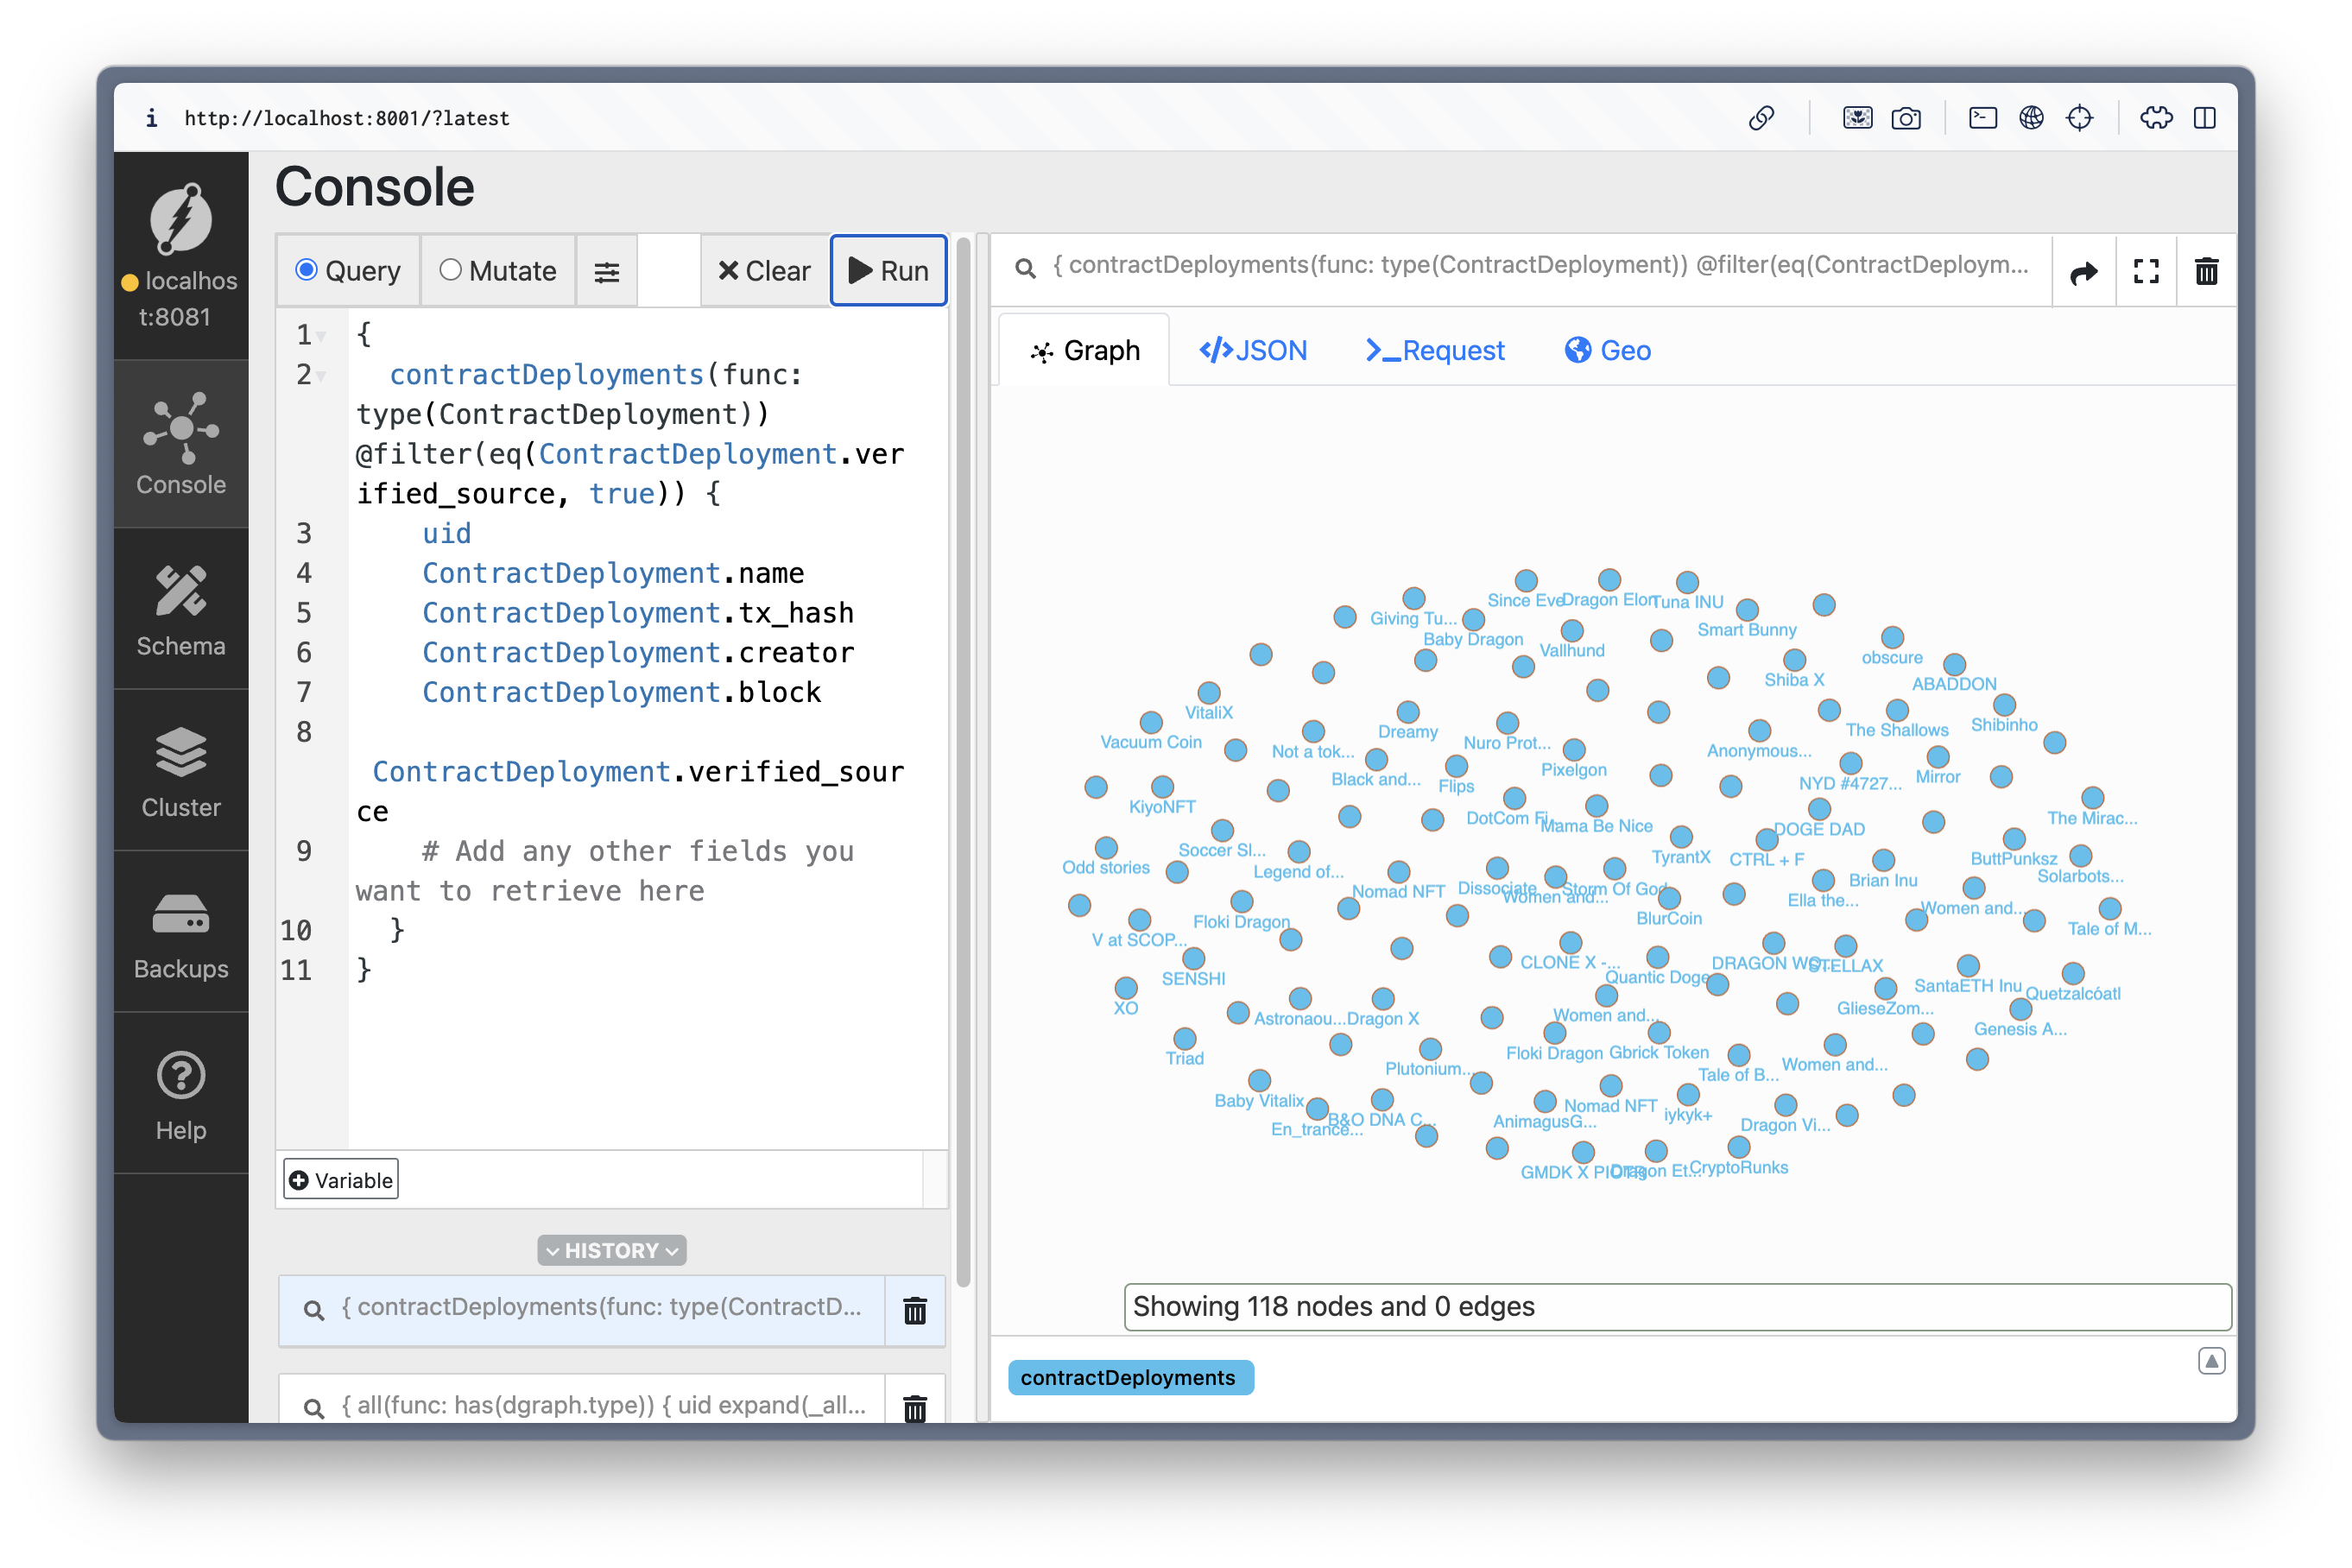
\includegraphics[width=1\textwidth]{resources/appendix/hasil-data-1.png}
	\caption{Hasil ekstraksi data}
	\label{image:hasil-data-1}
\end{figure}

\begin{figure}[ht]
	\centering
	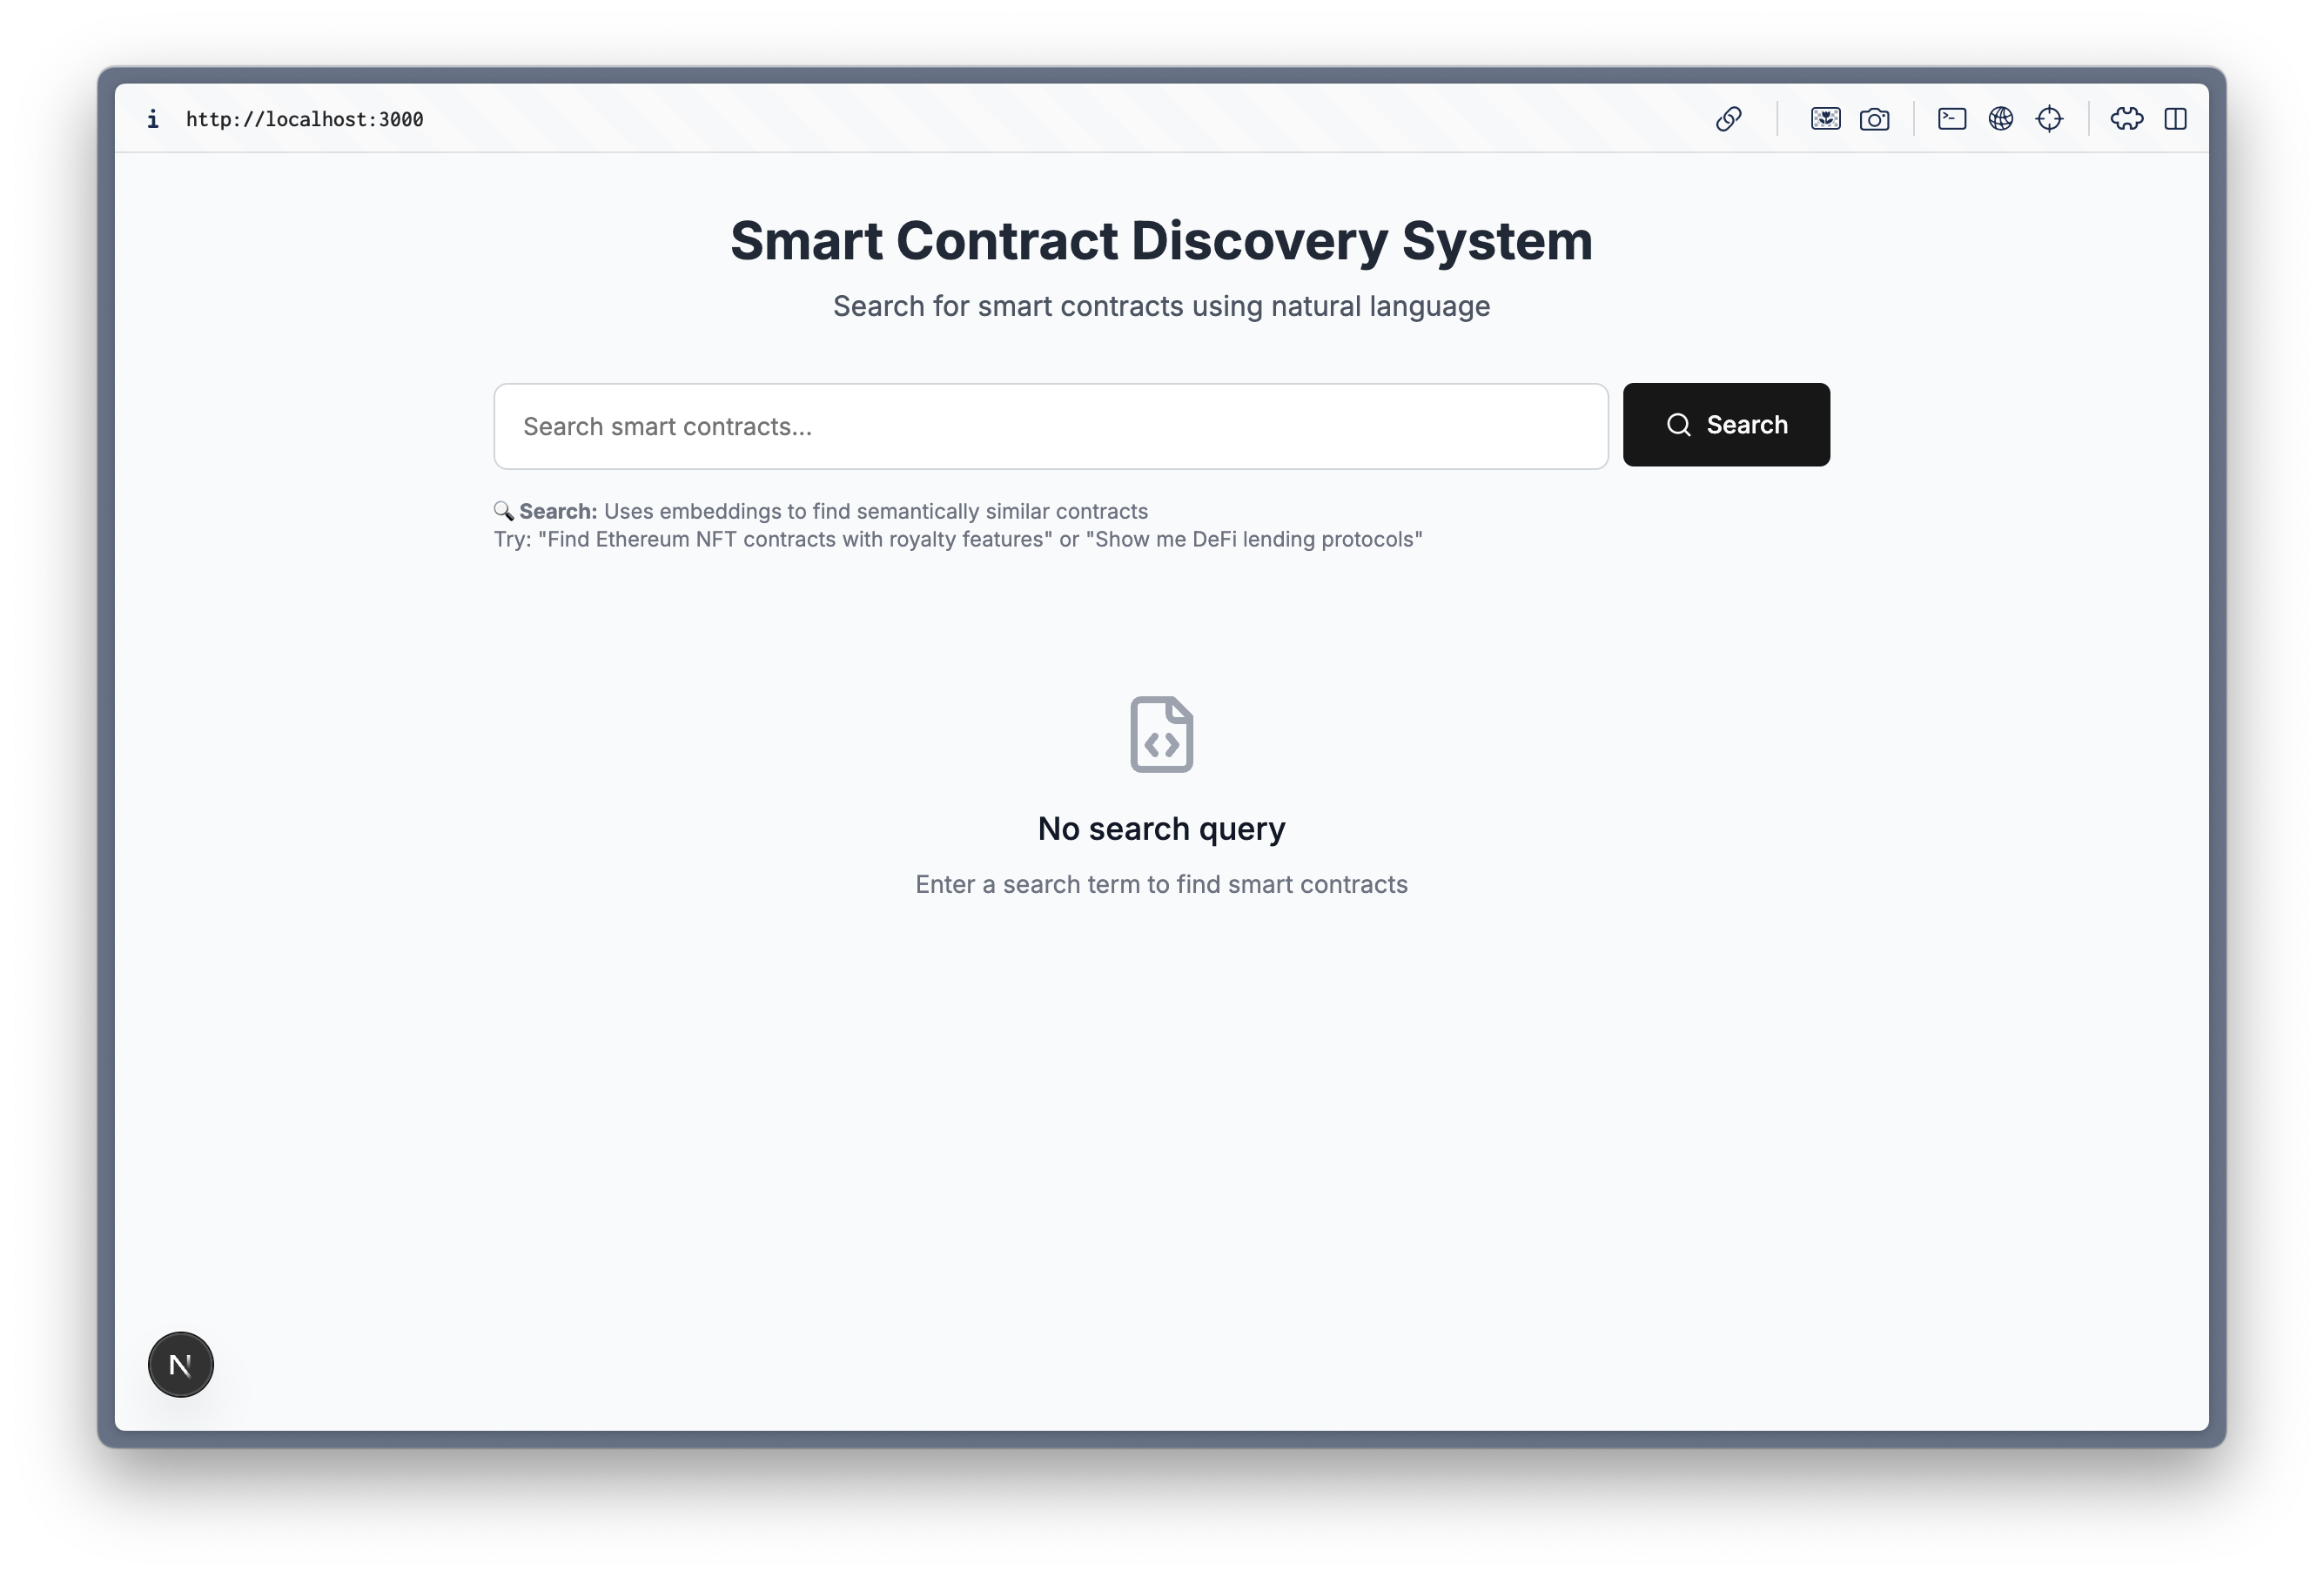
\includegraphics[width=1\textwidth]{resources/appendix/hasil-gui-1.png}
	\caption{Hasil antarmuka pengguna}
	\label{image:hasil-gui-1}
\end{figure}

\begin{figure}[ht]
	\centering
	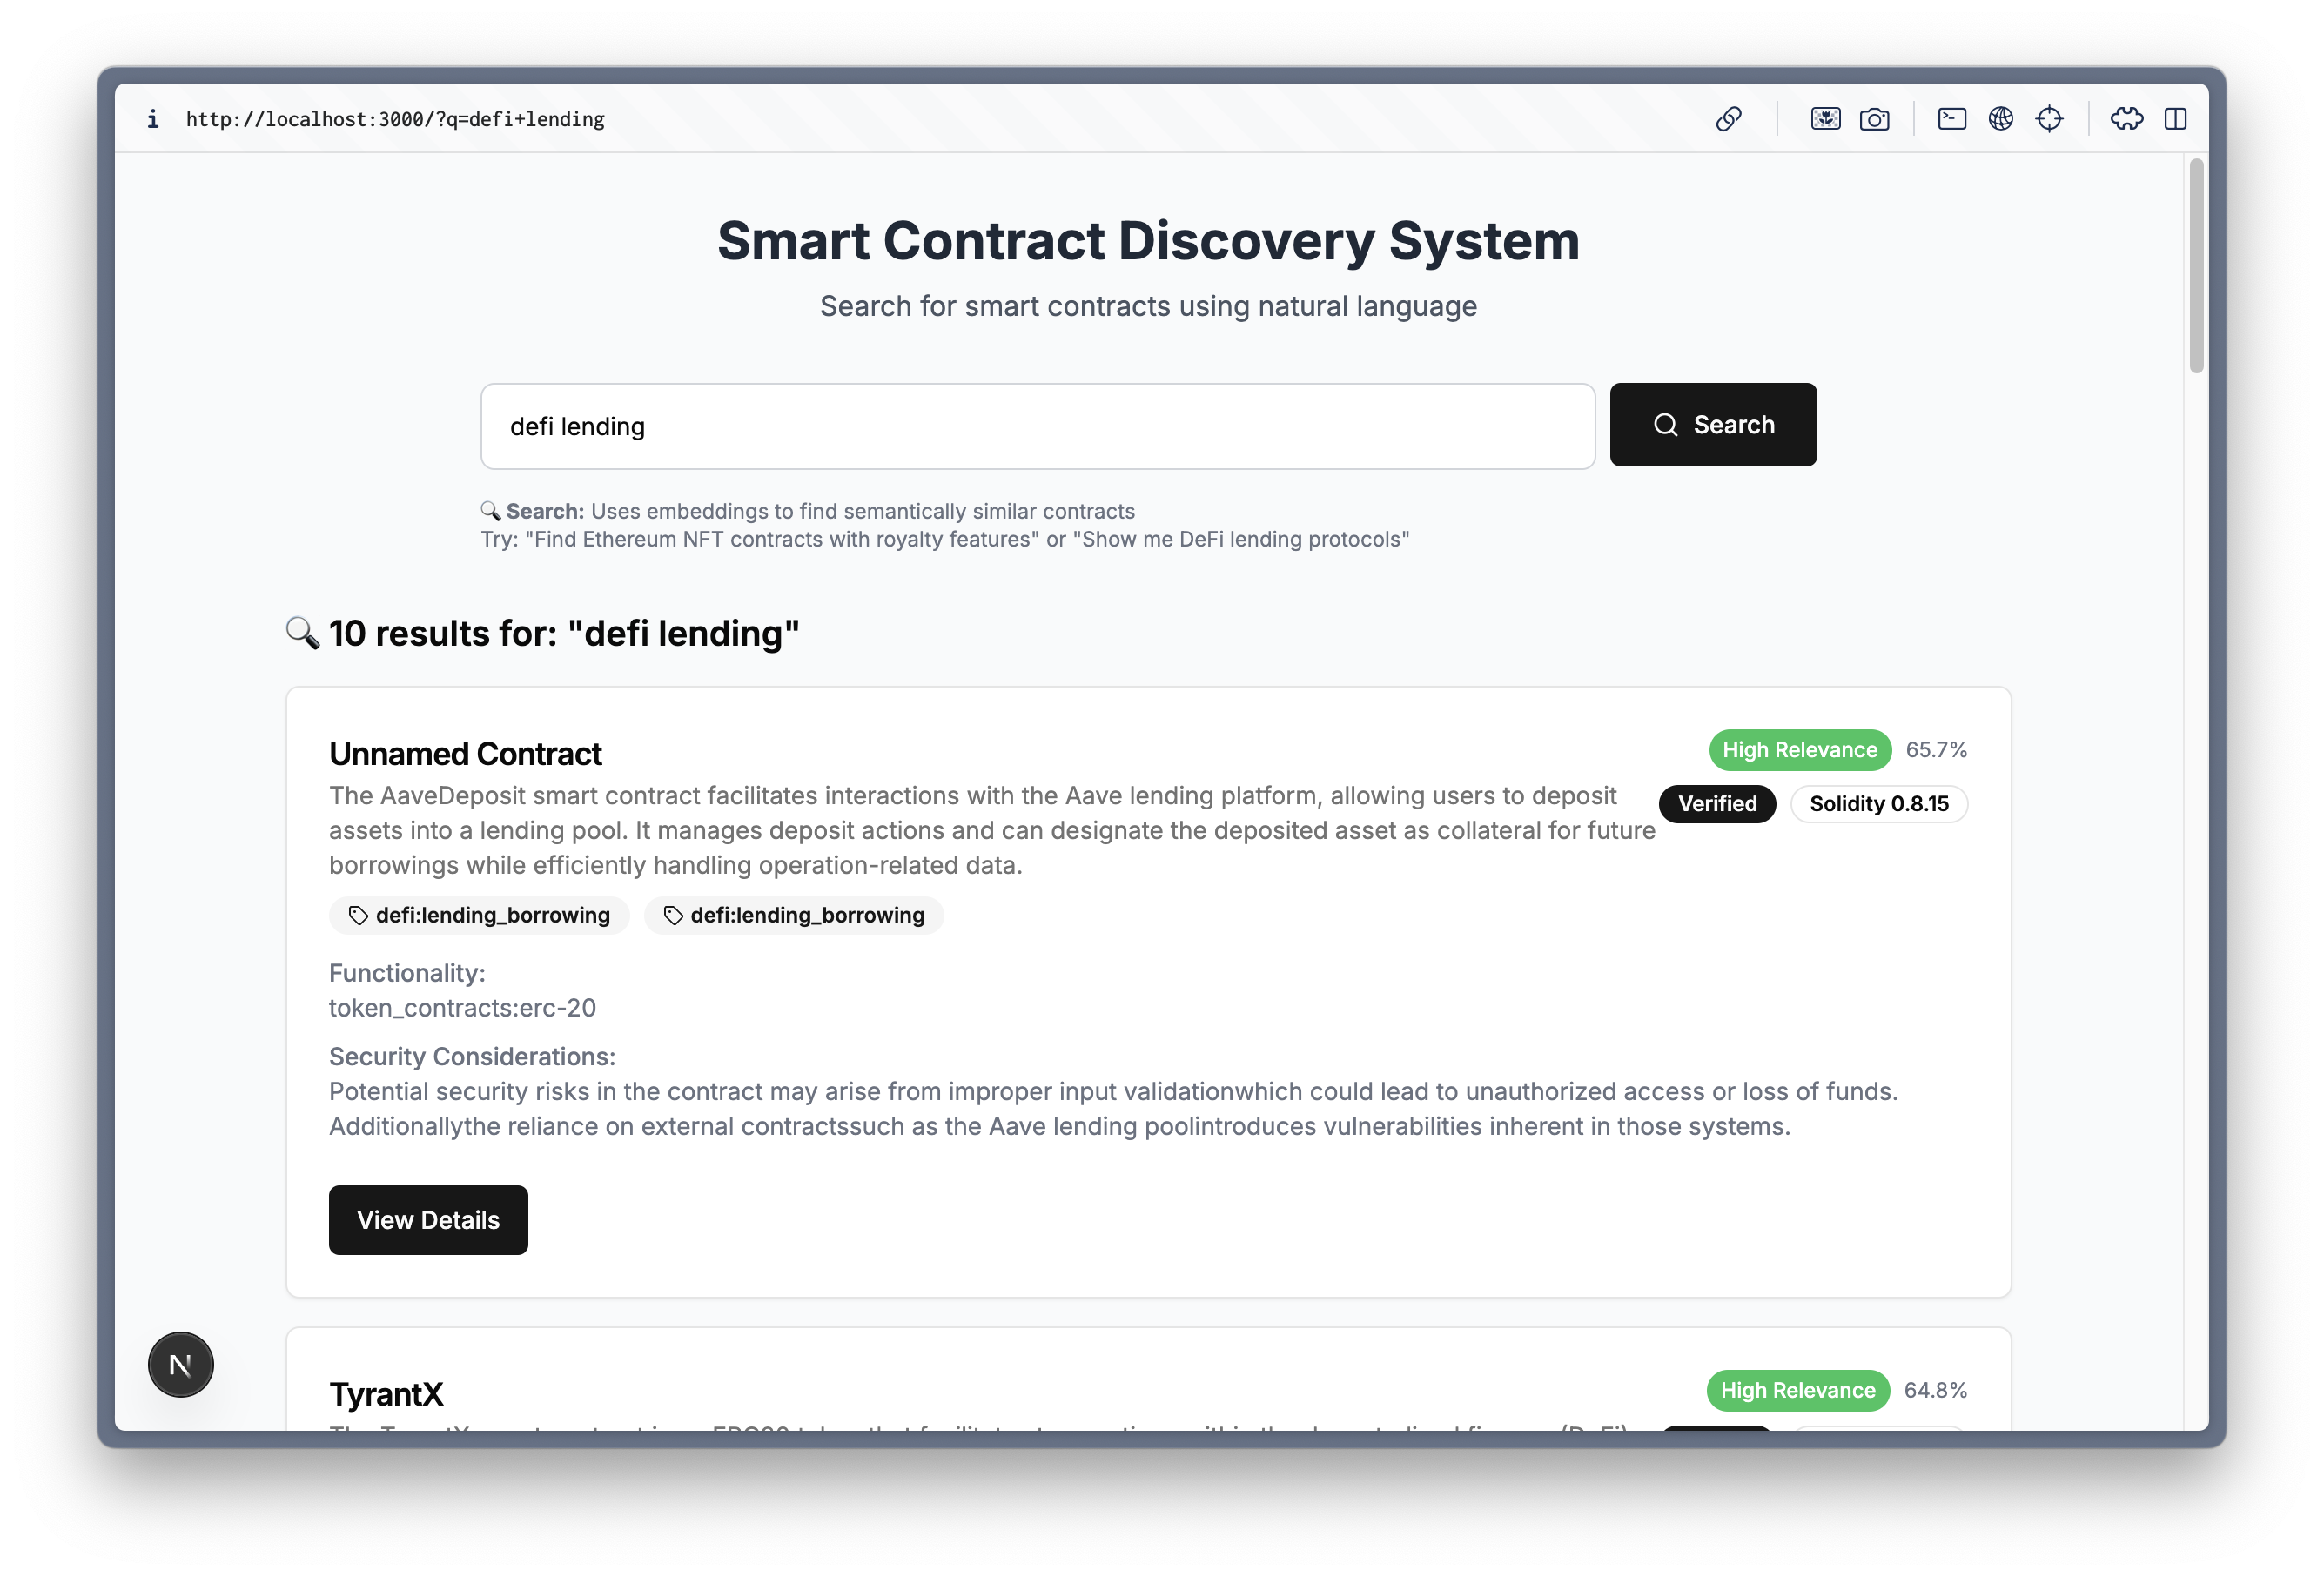
\includegraphics[width=1\textwidth]{resources/appendix/hasil-gui-2.png}
	\caption{Hasil antarmuka pengguna}
	\label{image:hasil-gui-2}
\end{figure}

\begin{figure}[ht]
	\centering
	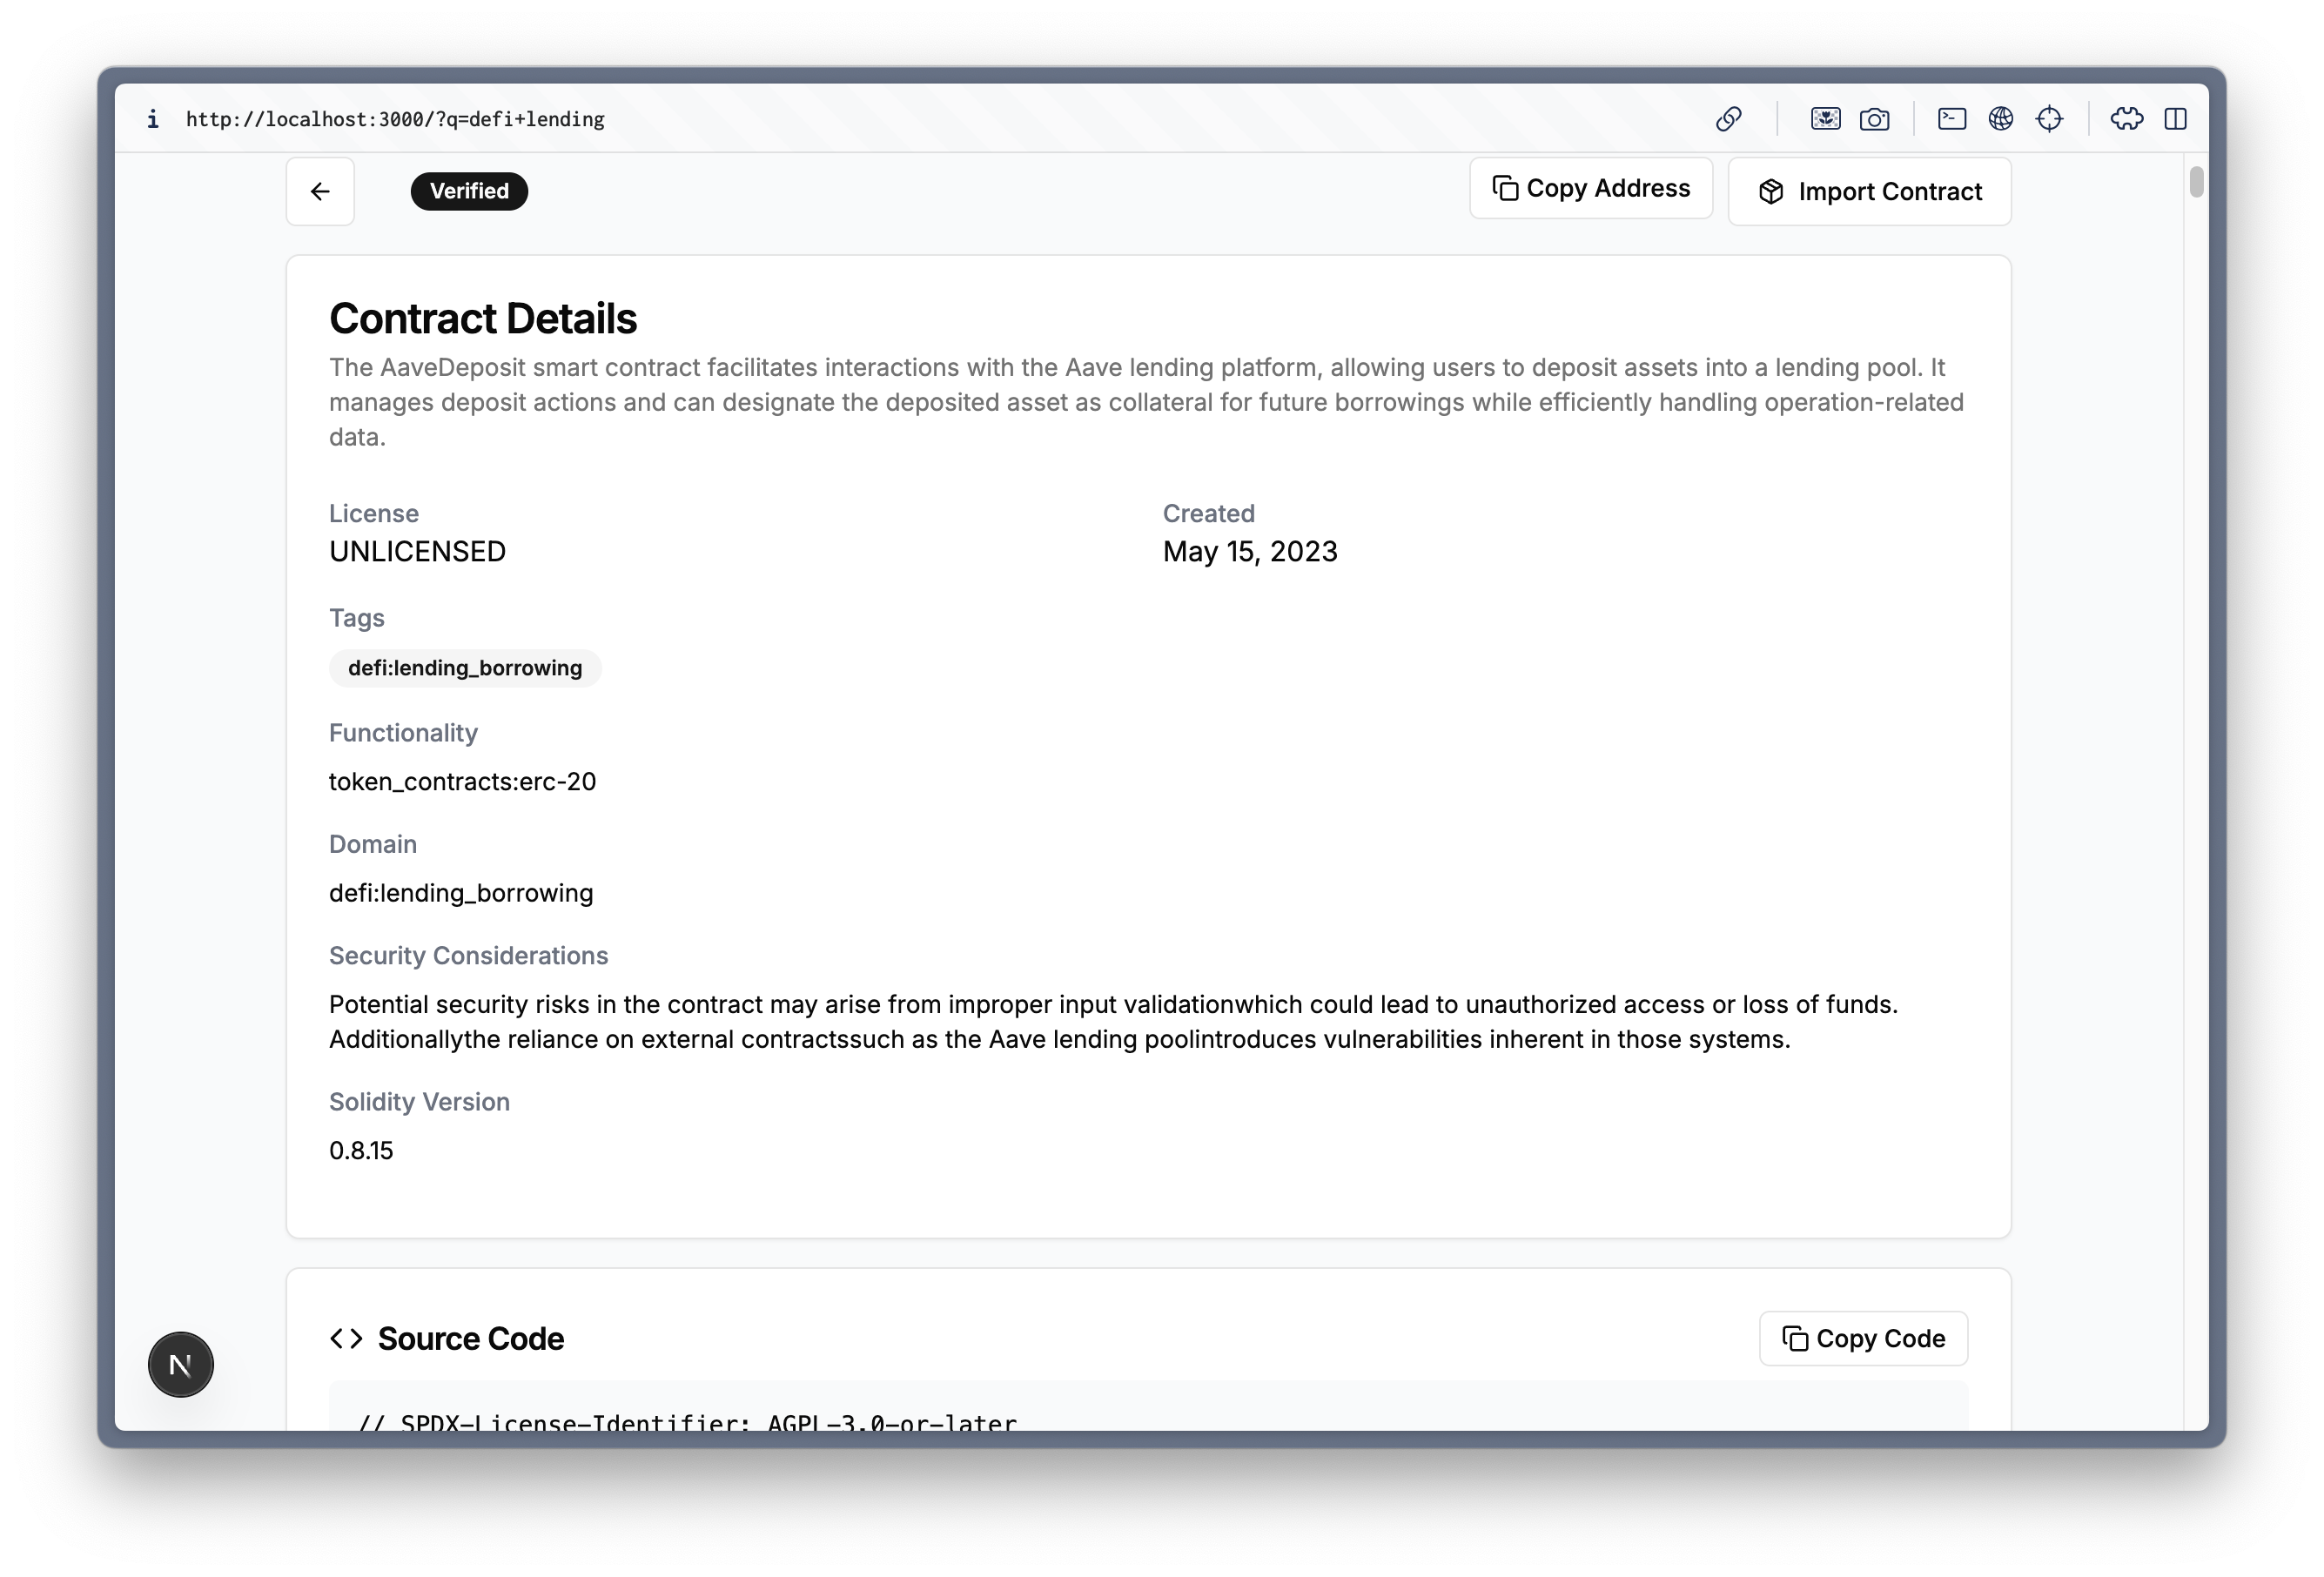
\includegraphics[width=1\textwidth]{resources/appendix/hasil-gui-3.png}
	\caption{Hasil antarmuka pengguna}
	\label{image:hasil-gui-3}
\end{figure}

\begin{figure}[ht]
	\centering
	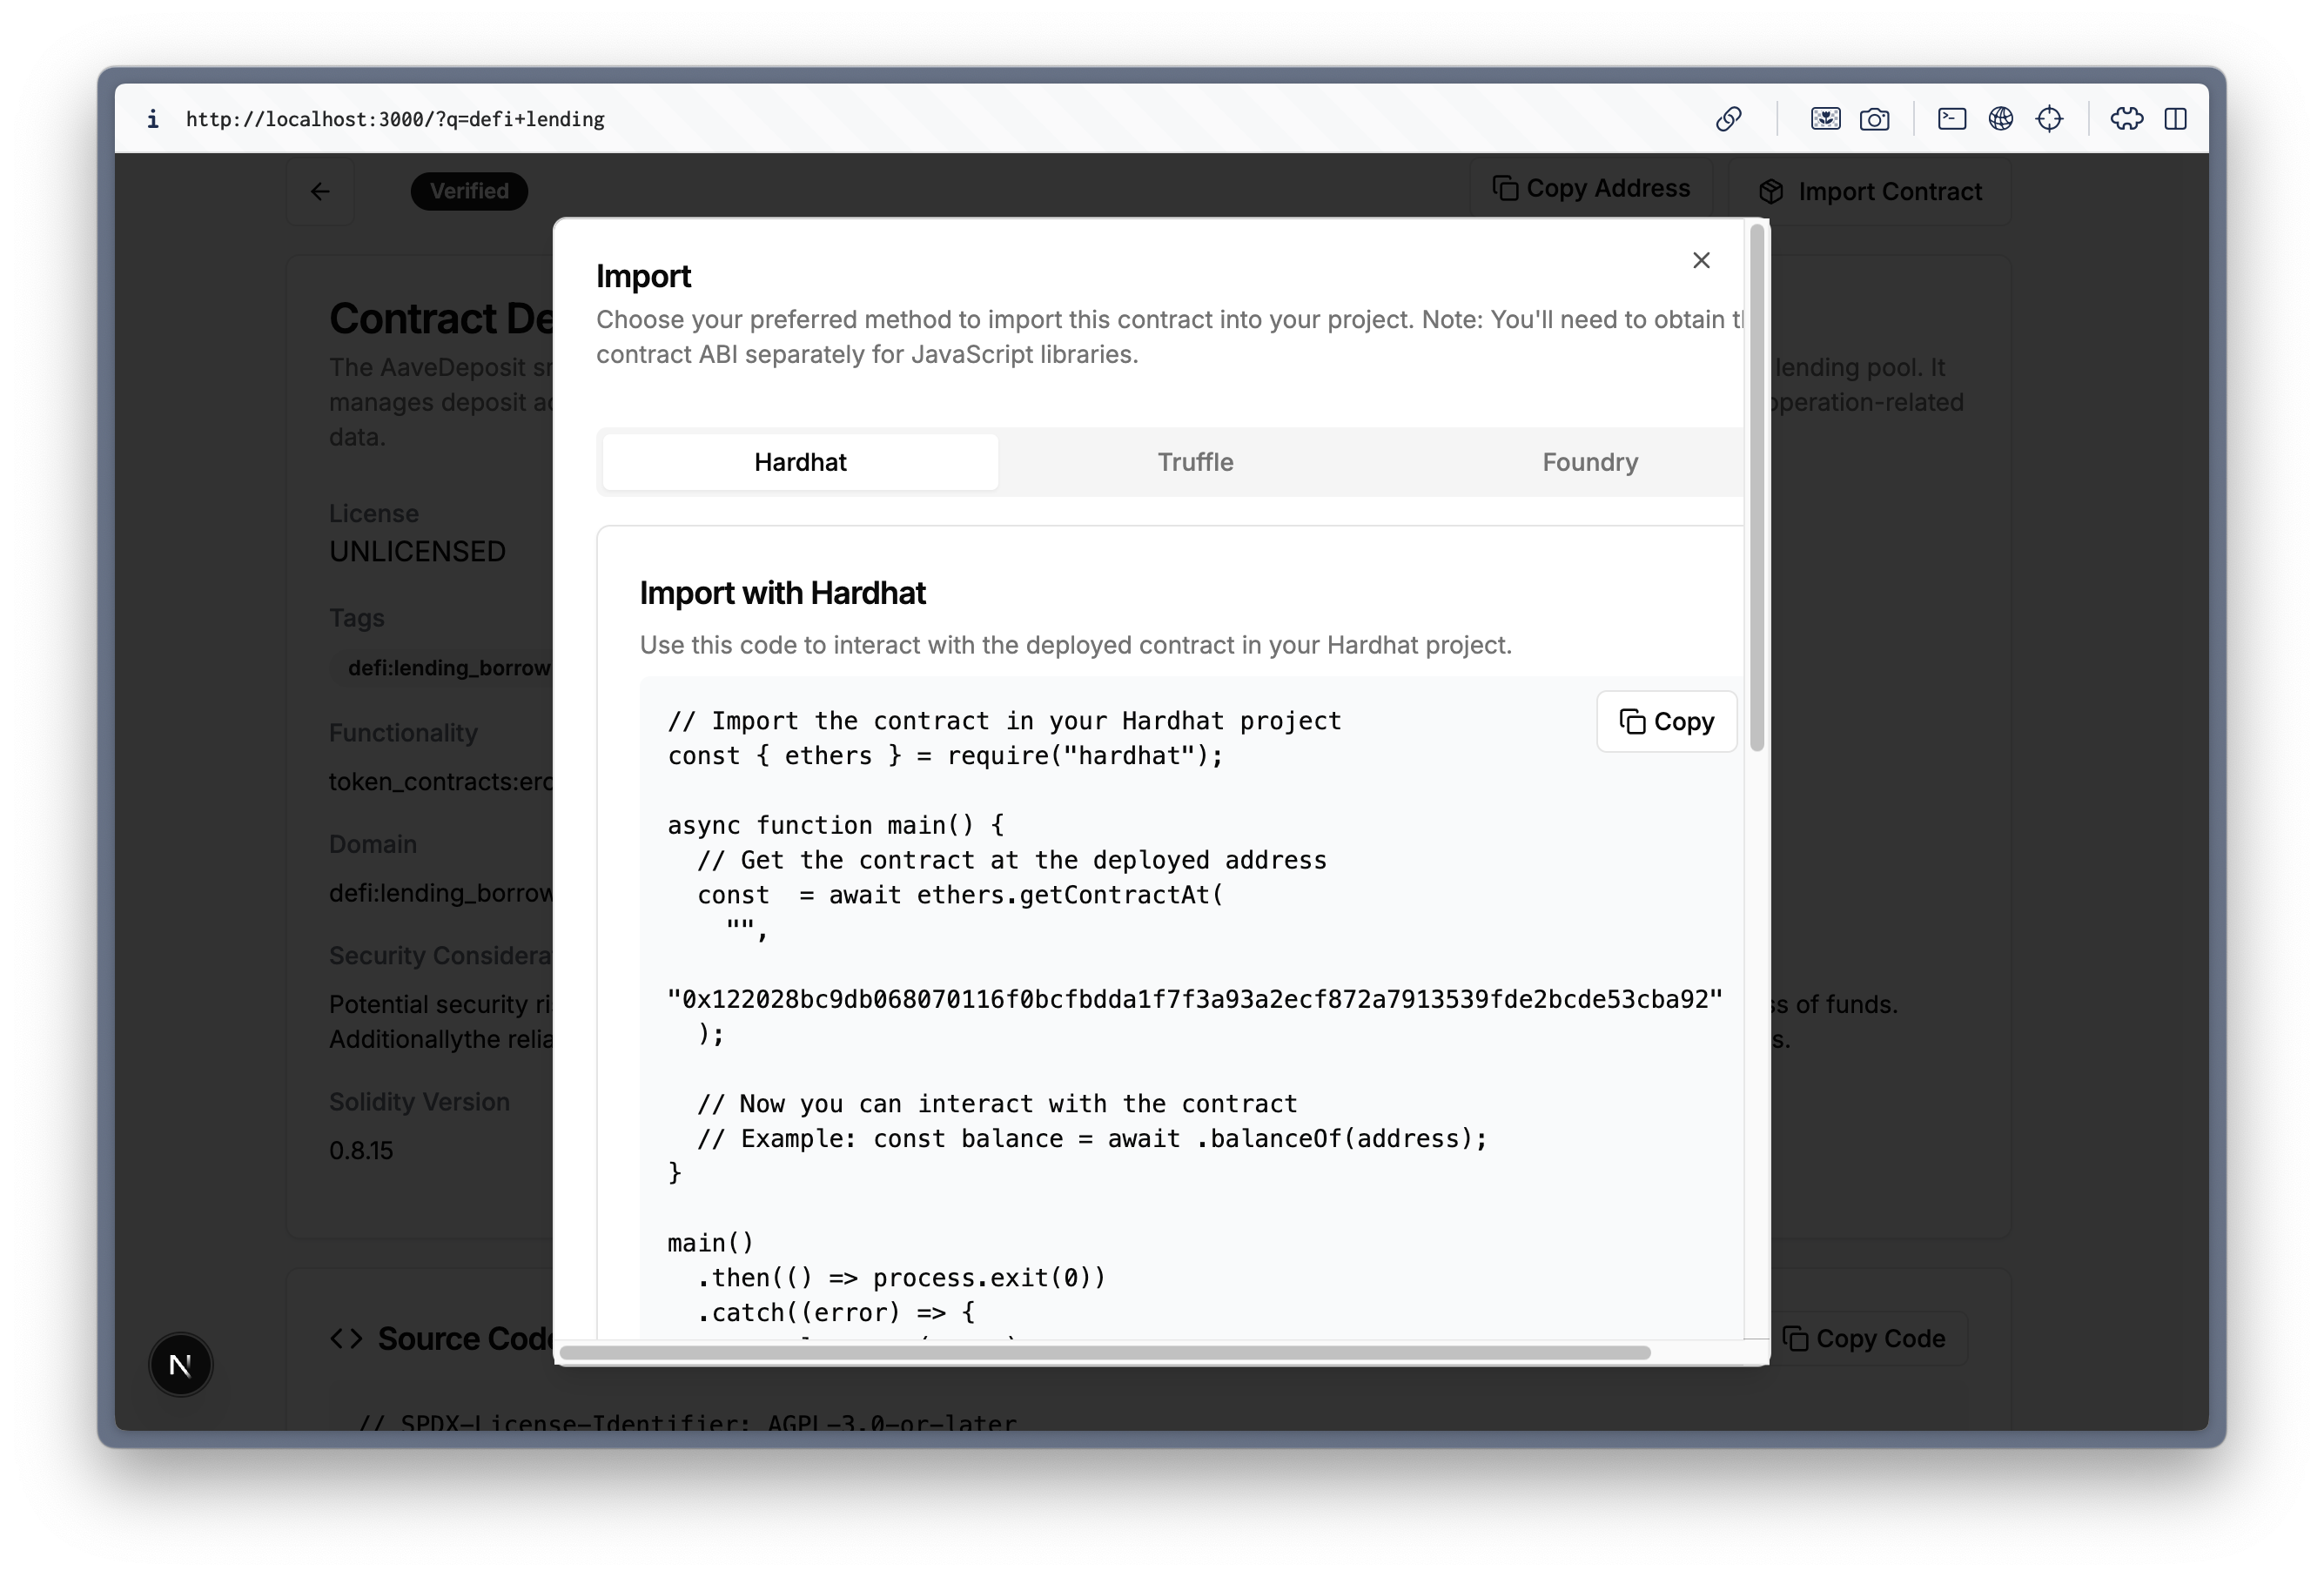
\includegraphics[width=1\textwidth]{resources/appendix/hasil-gui-4.png}
	\caption{Hasil antarmuka pengguna}
	\label{image:hasil-gui-4}
\end{figure}

\begin{figure}[ht]
	\centering
	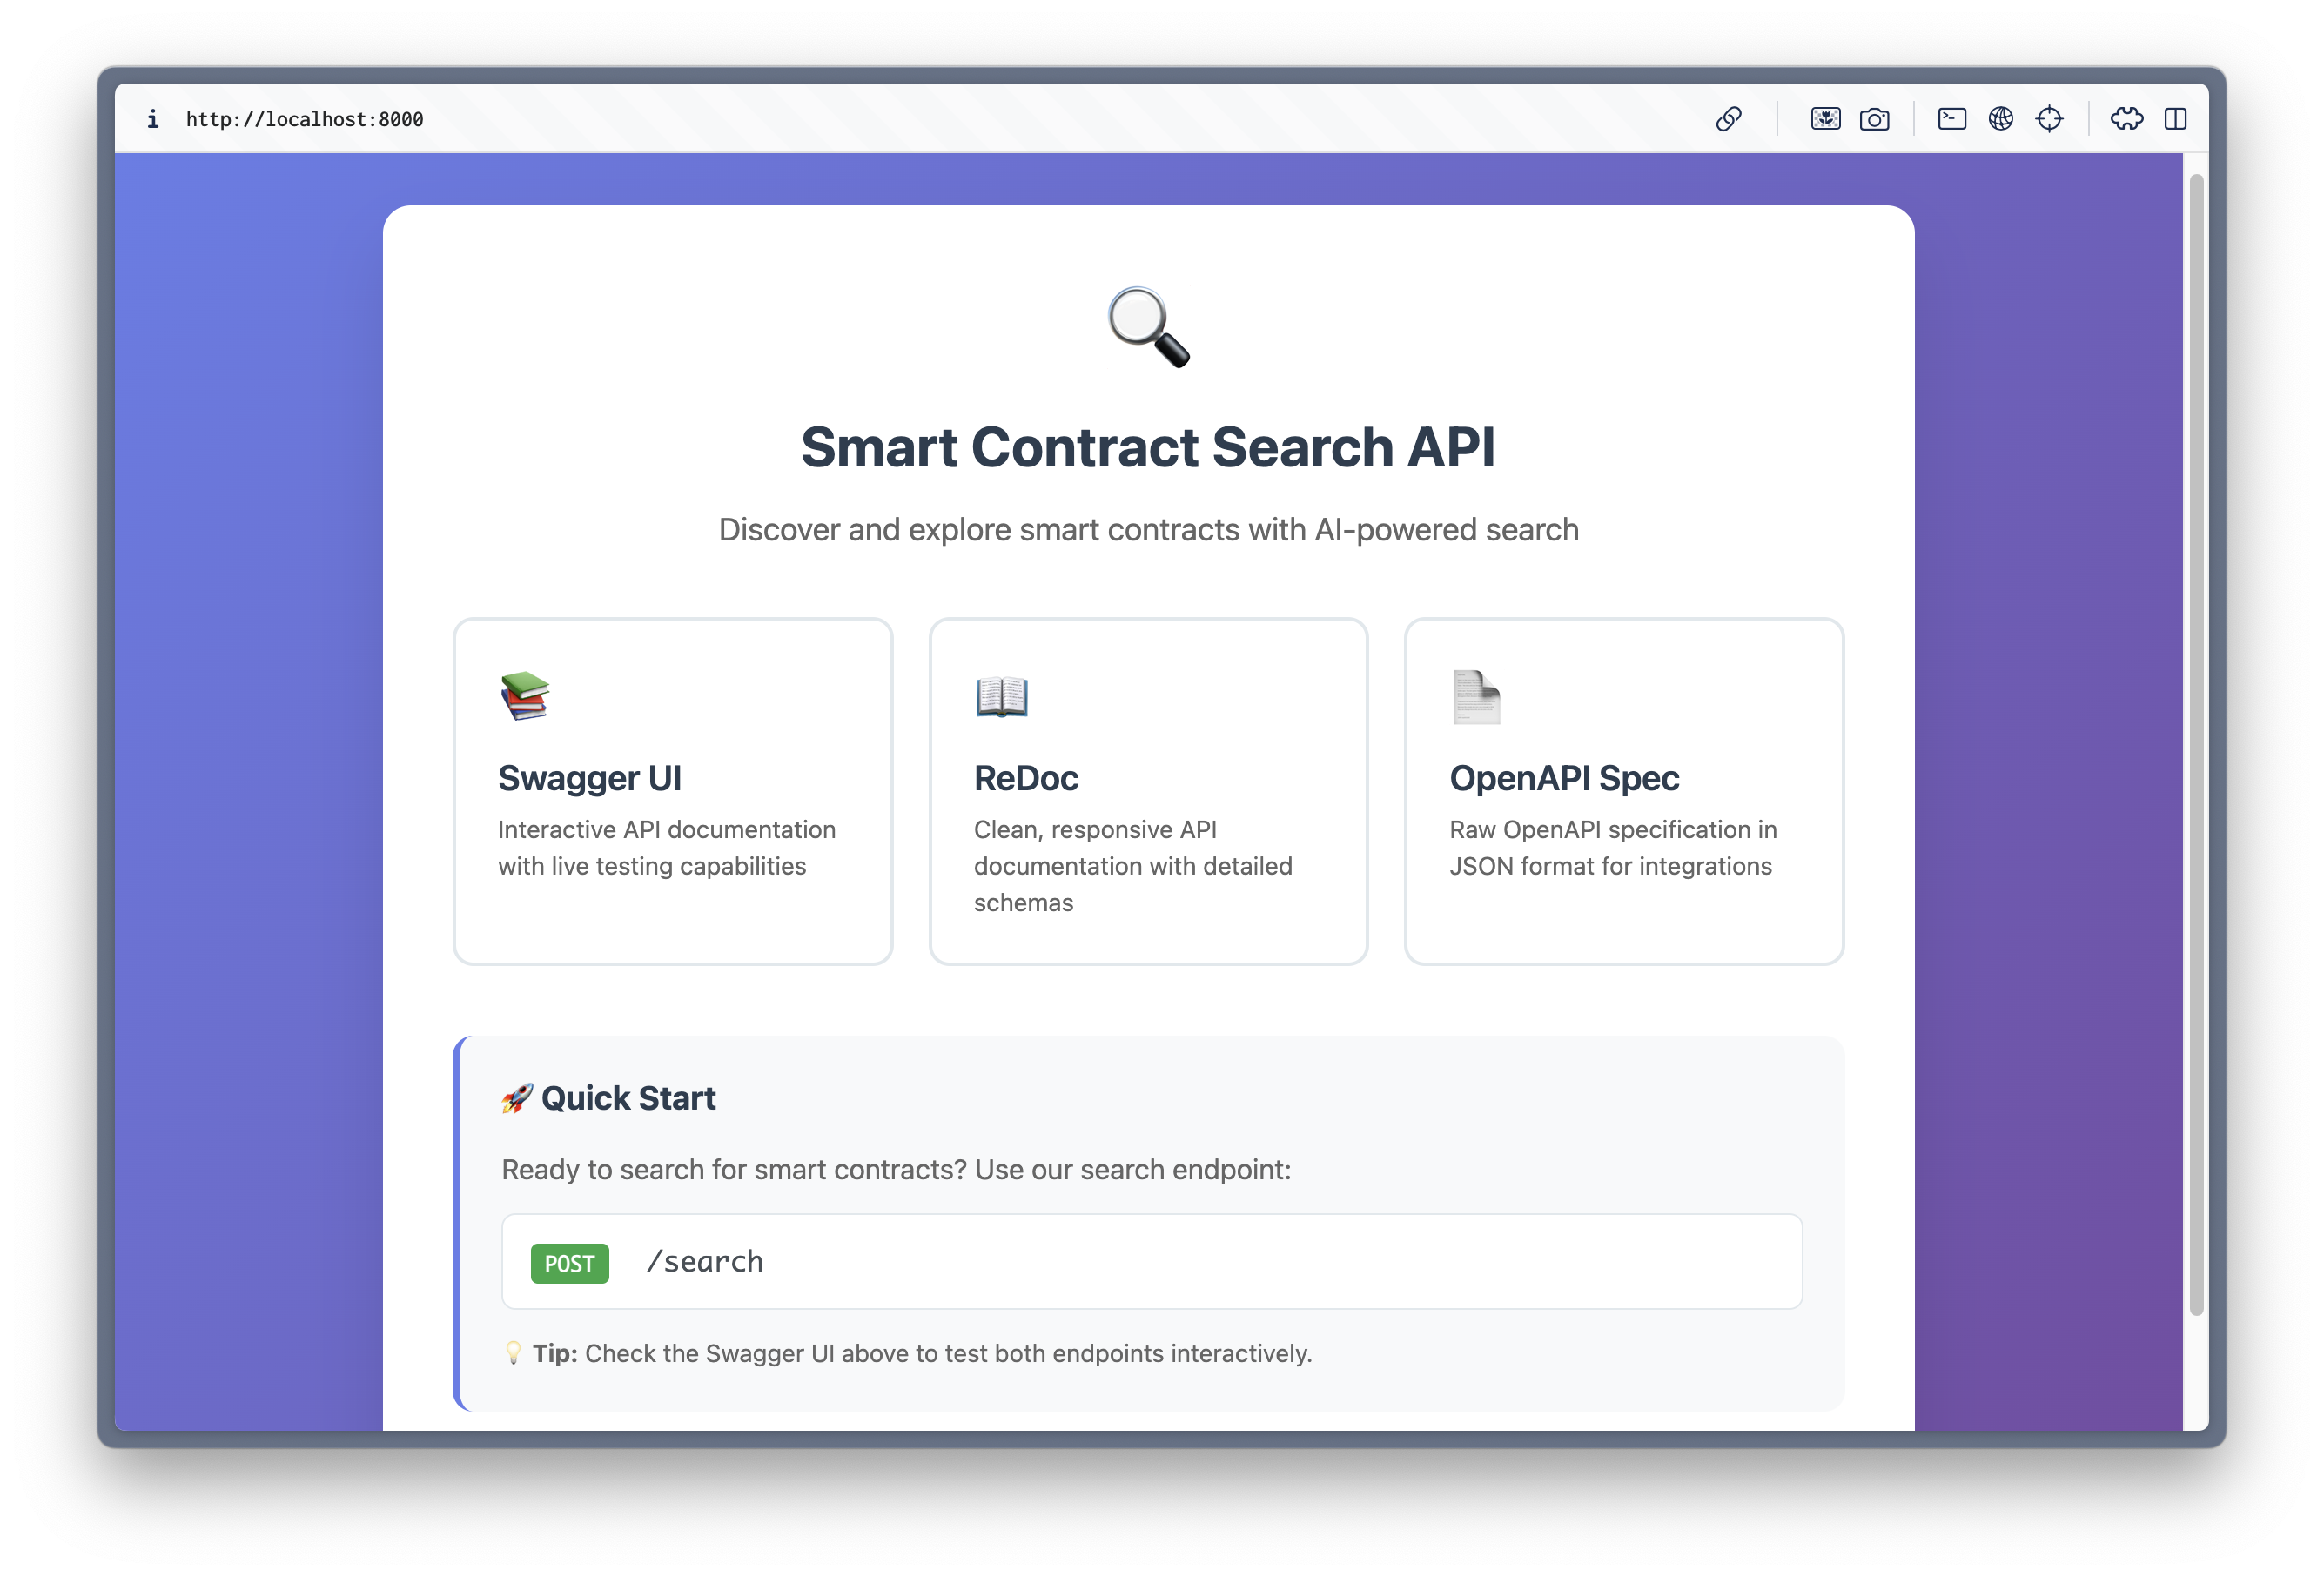
\includegraphics[width=1\textwidth]{resources/appendix/hasil-api-1.png}
	\caption{Hasil antarmuka pengguna}
	\label{image:hasil-api-1}
\end{figure}

\begin{figure}[ht]
	\centering
	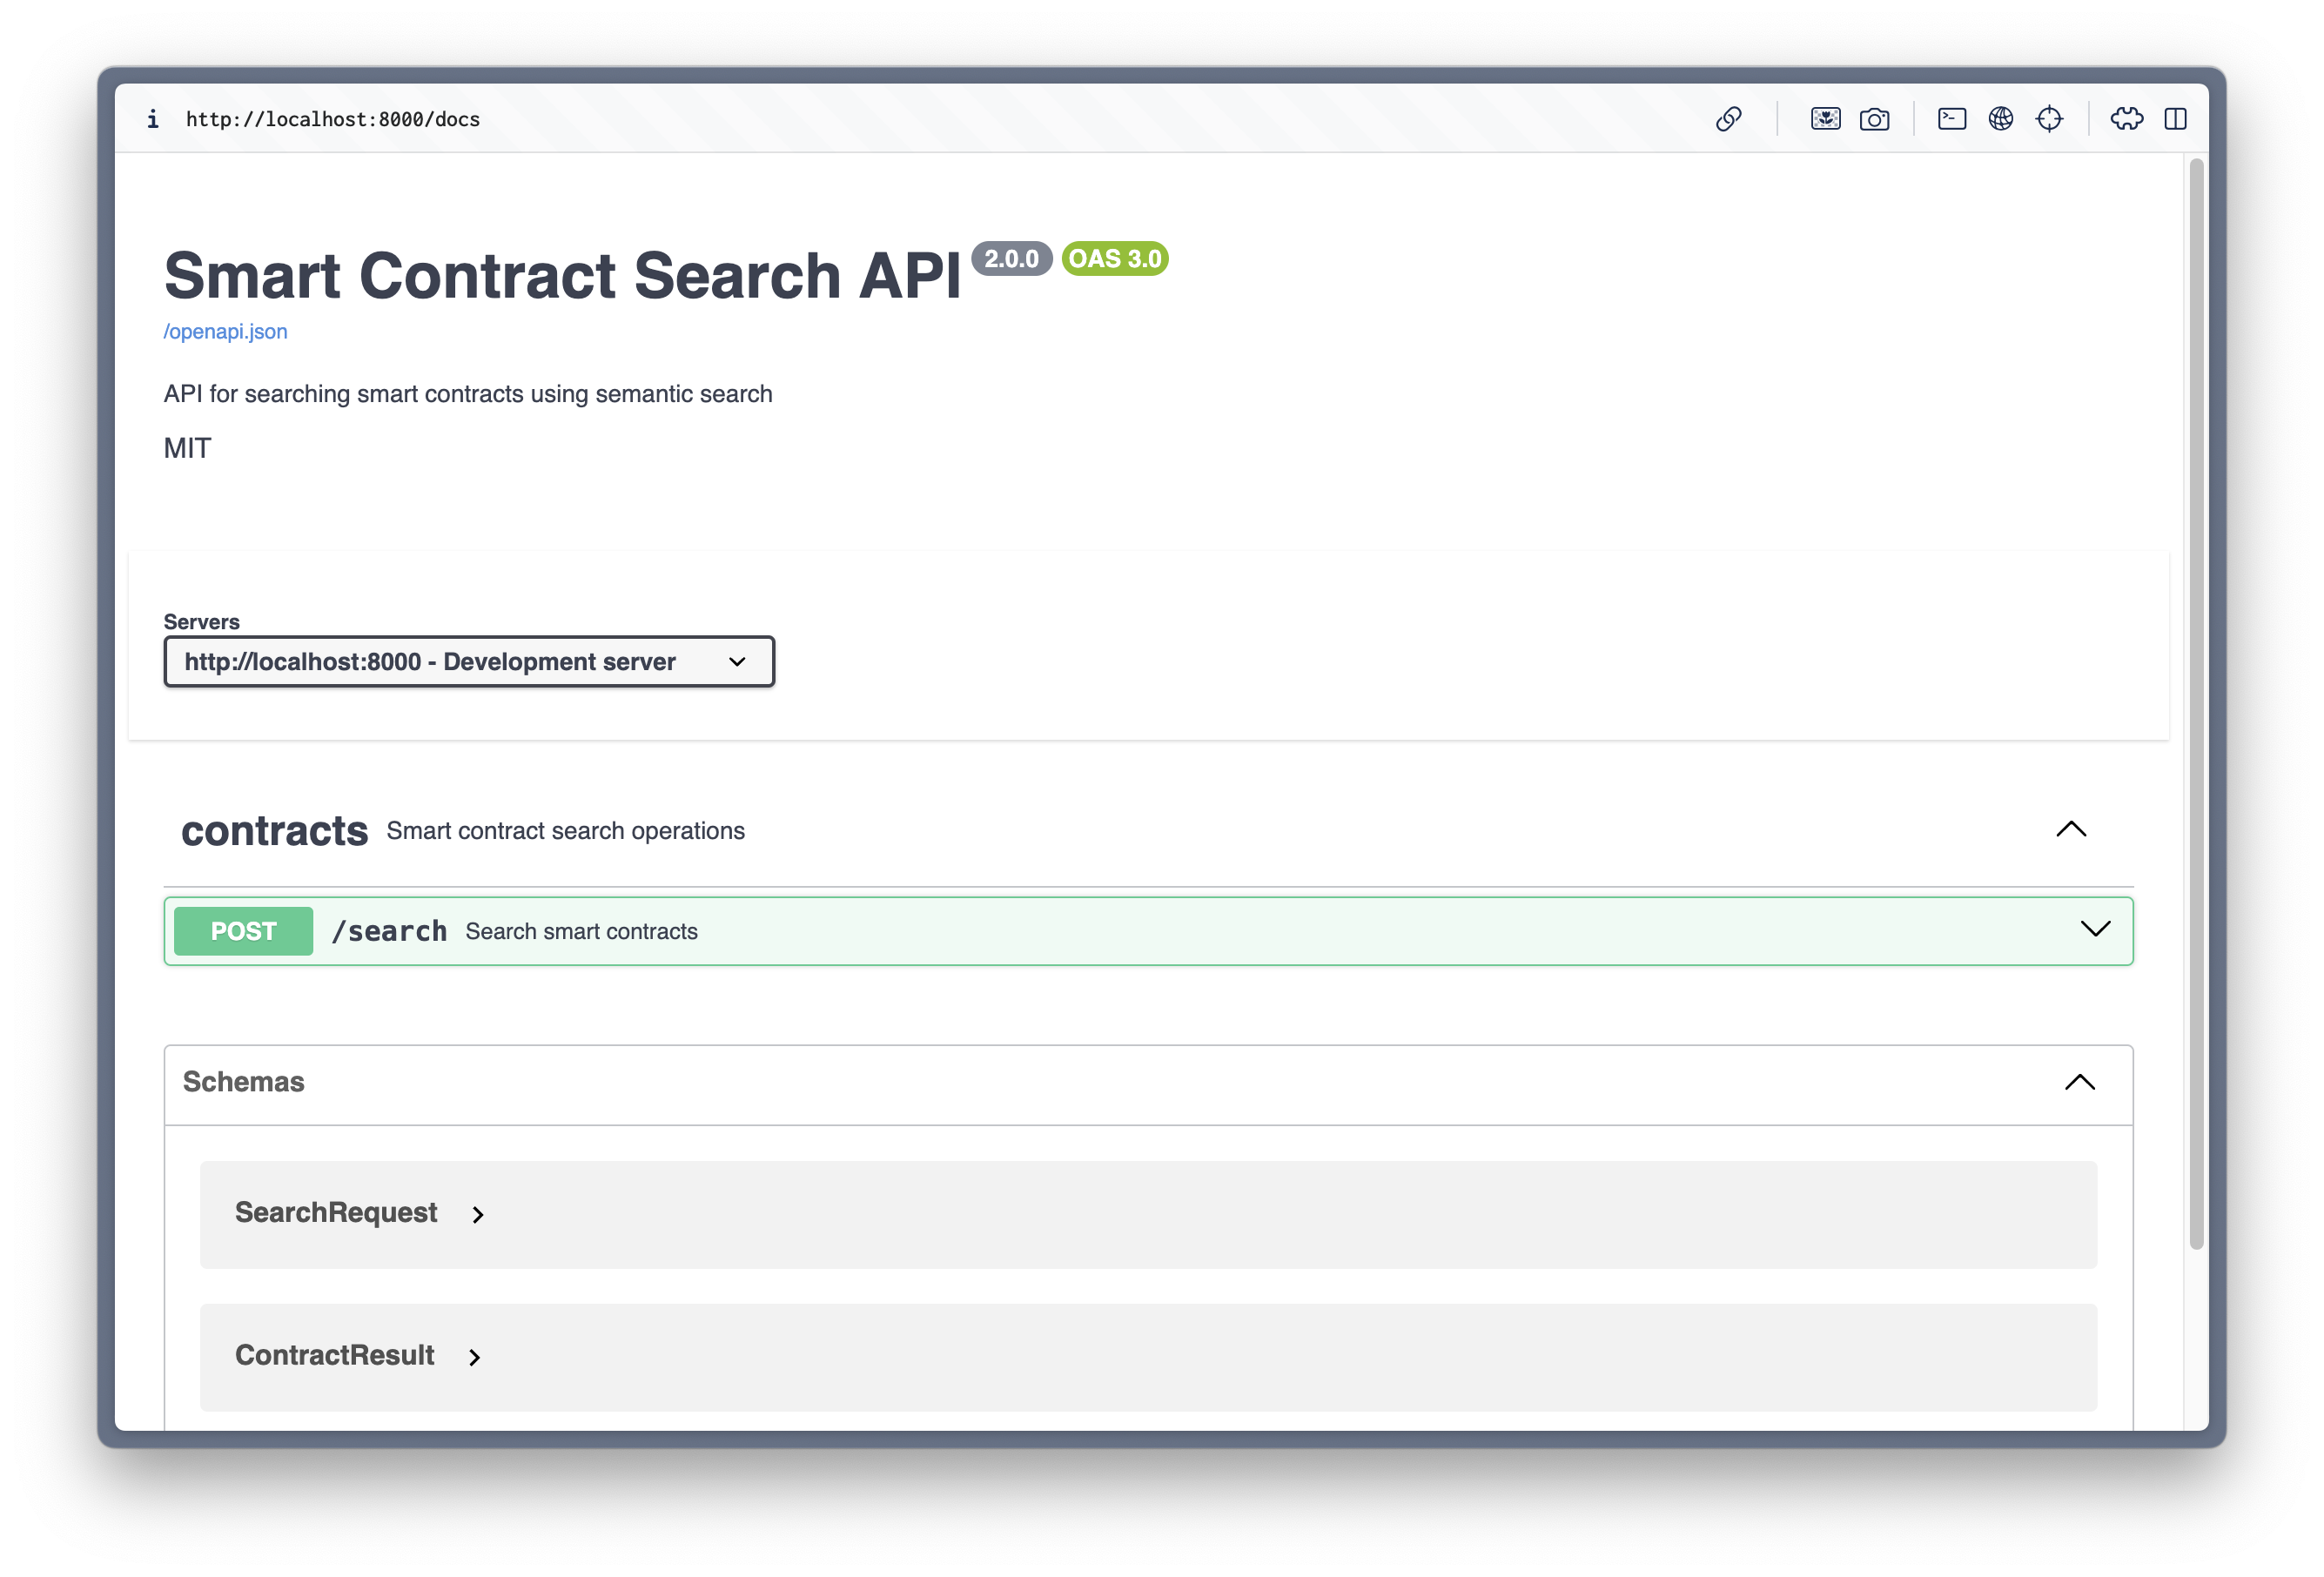
\includegraphics[width=1\textwidth]{resources/appendix/hasil-api-2.png}
	\caption{Hasil antarmuka pengguna}
	\label{image:hasil-api-2}
\end{figure}

\begin{figure}[ht]
	\centering
	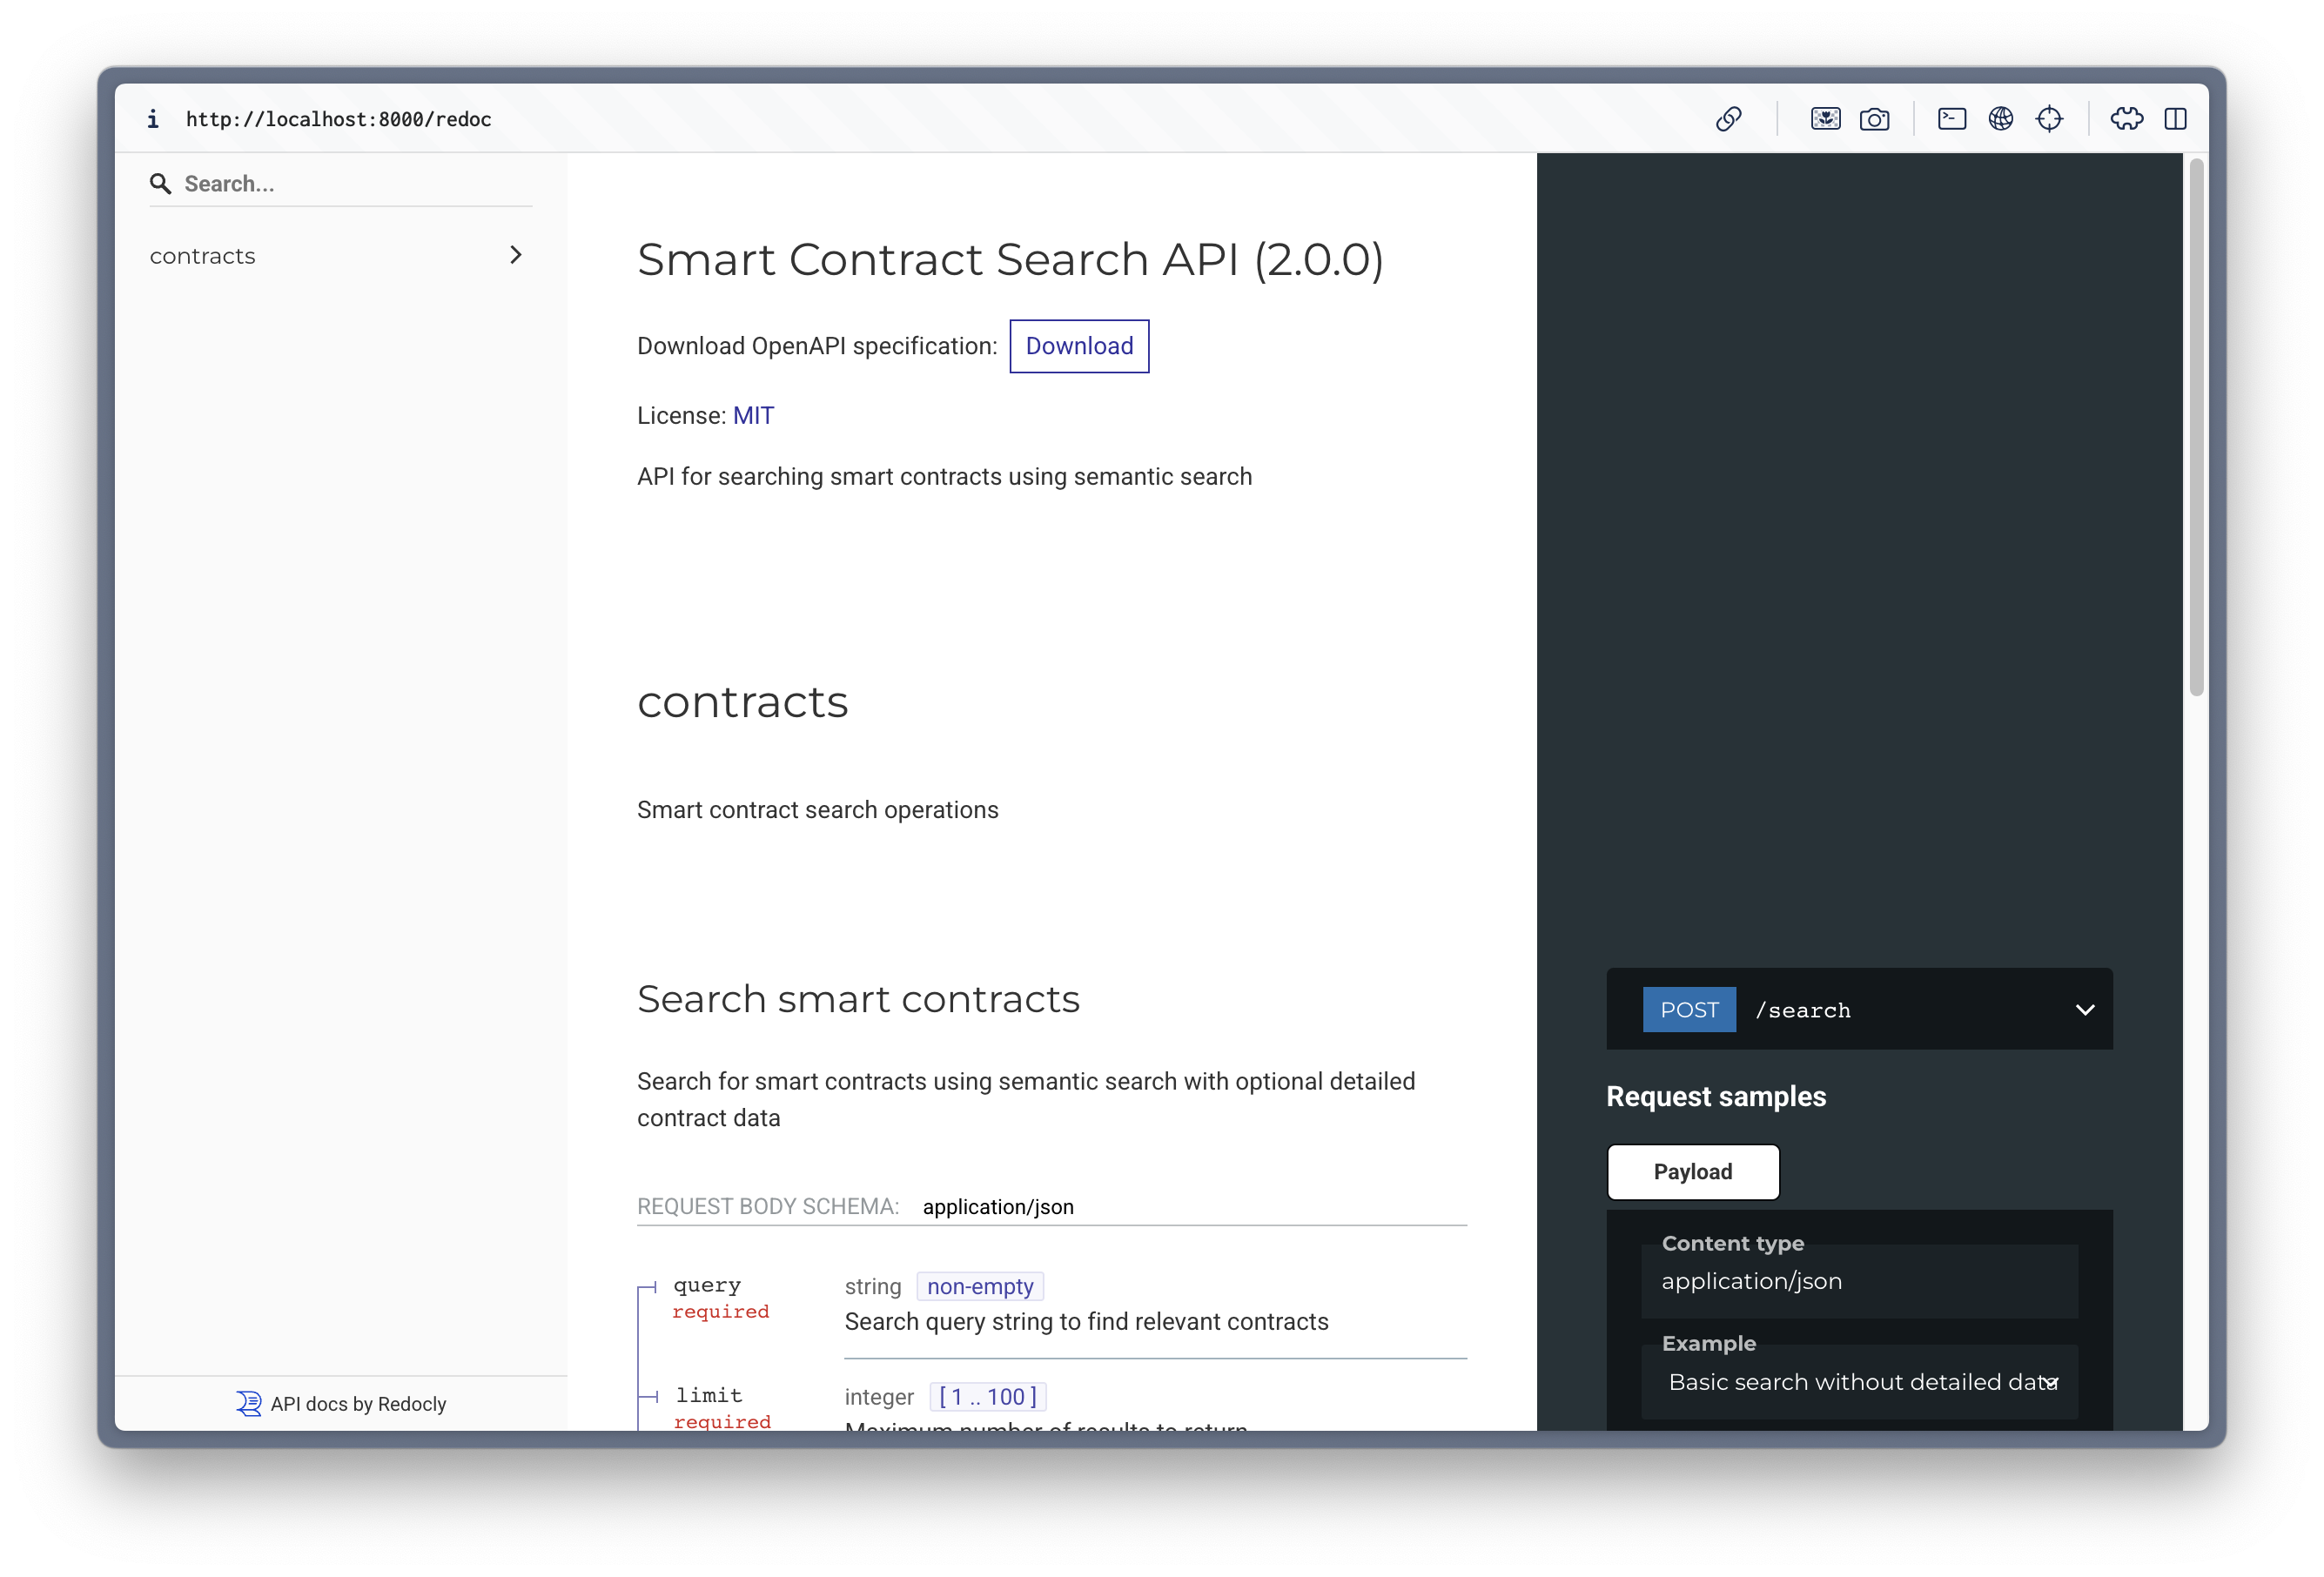
\includegraphics[width=1\textwidth]{resources/appendix/hasil-api-3.png}
	\caption{Hasil antarmuka pengguna}
	\label{image:hasil-api-3}
\end{figure}


\end{document}
